\documentclass[11pt]{article}
\author{Adrian Mircea Nenu}

\usepackage[utf8]{inputenc}
\usepackage{titling}
\usepackage{amssymb}
\usepackage{geometry} 
\geometry{a4paper}
\usepackage{graphicx}
\usepackage{hyperref}
\usepackage{wrapfig}
\usepackage{float}
\usepackage{comment}
\usepackage{hyperref}
\usepackage{listings}
\usepackage{tabu}
\usepackage{longtable}
\usepackage{color}
\usepackage[table, svgnames]{xcolor}
\usepackage{array}
\usepackage{minted}
\usepackage{amsmath}
\usepackage{tikz}
\usepackage[page,toc,titletoc,title]{appendix}

\usepackage[
backend=biber,
sorting=ynt
]{biblatex}
\usepackage{etoolbox}
\addbibresource{my.bib}


\lstset{
  basicstyle=\ttfamily\tiny,
  breaklines=true,
  columns=fullflexible,
  keywordstyle=\color[rgb]{0,0,1},
  commentstyle=\color[rgb]{0.133,0.545,0.133},
  stringstyle=\color[rgb]{0.627,0.126,0.941}
}

\renewcommand*\contentsname{Table of Contents}

\AtBeginEnvironment{tabular}{\rowcolors{1}{\ifnumless{\rownum}{2}{DarkSeaGreen!40}{white}}{}}
\renewcommand{\arraystretch}{2}
 
\begin{document}

\begin{center}
    ~\\ 
    
\includegraphics[width=8cm]{img/bath.jpg} 
 
    ~\\  
    ~\\ 
    ~\\ 
    ~\\ 
    ~\\ 
    \small Adrian-Mircea Nenu
    ~\\ 
    \small Supervisor: Dr Sheik Meeran
    ~\\ 
    ~\\ 
    \large MSc in Business Analytics
    ~\\ 
    \Huge Stock Clustering of S\&P 500 and NASDAQ 100 Constituents for Investment Strategy Optimisation  
    ~\\ 
    ~\\ 
    ~\\ 
    ~\\    
            ~\\    
    ~\\    
    ~\\    
    \Large October, 2023
    ~\\    
    ~\\    
    \large Submitted as part of the requirement for completing an \\
    MSc in Business Analytics at the University of Bath
    ~\\    
    ~\\    
    \small 12,000 words
\end{center}

\thispagestyle{empty}

\newpage


\begin{center} {\LARGE Abstract} \end{center}

Recognising inherent patterns is a foundational stage in the crafting of risk-mitigating and diversified investment strategies. Conventional methods for analysing stocks, such as linear regression and principal component analysis (PCA), possess limitations in terms of their capacity to identify non-linear (non-euclidean) relationships and overlook asynchronous intricate patterns within the data that are often hard to identify without human subjective oversight. This research explores the use of clustering as having the potential to provide strong signals for analysing stock prices in order to identify asynchronous patterns of similarities between them. We have explored diverse methodologies for computing distances such as Euclidean, Dynamic Time Warping (DTW) and Self-Organising Maps (SOM).

DTW, as a non-linear technique, facilitates the alignment of time-series even in the presence of non-uniform time axes, allowing us to discover correlations between cross-industry stocks that otherwise might not have been apparent.

Self-Organising Maps are a type of unsupervised artificial neural network which would be well suited for higher dimensional data than we have explored but deliver in our results the smoothest trends.

Through this research, we apply the selected algorithms on a data-set bringing together historical stock prices of top S\&P 500 and NASDAQ companies. We employ a series of methodologies for creating a similarity analysis for defining the distance between the stocks for clustering. The clusters serve the purpose of identifying and scrutinising similarly behaving stocks, thus playing a crucial role in informing a potential investment strategy formulation.

To gauge the effectiveness of these methodologies we have a series of pre-established metrics consistently recorded for each algorithm: Silhouette score, Calinski-Harabasz index, Davies-Bouldin index, and visual observations. Due to the inherent complexity of non-euclidean pattern finding, we have extensively relied on visual analysis of clusters alongside empirical mathematical metrics.

Backtesting and portfolio assessment algorithms have not been applied but would be the next logical step following our results to assign a monetary value to the improvements provided by these algorithms. The results of such an assessment would depend heavily on how the algorithms are integrated in the holistic investment strategy more than their individual independent efficacy.


\newpage

\begin{center} {\LARGE Acknowledgements} \end{center}

I would like to thank my supervisor, Dr Sheik Meeran, for his support of the project and for making sure I stayed on track regardless of other competing goals, thanks to which I have been empowered to manage my time effectively and ensure that I understand all the milestones involved.

 I want to express my gratitude to the distinguished professors from the University of Bath who have contributed their remarkable insights and teachings during my academic journey in pursuing my Master of Science degree in Business Analytics. Their collective expertise and guidance have broadened my perspective and enriched my knowledge in this field.

 Last, but not least, I give my sincere gratitude to my parents and fiancée for their unconditional support and encouragement throughout my academic pursuits. Their love and unwavering belief in my abilities have been a constant source of motivation and inspiration, encouraging me to strive for excellence and reach my goals.
\newpage

\tableofcontents

\newpage

\section{Tables and Figures}

\listoftables

\listoffigures

\newpage

\section{Problem Definition}

The global financial system is a core and notoriously dynamic part of human society, and it is a field of interest for many who seek out strategies to inform the decision-making process for making thoughtful investments. 

Understanding and predicting historical trends in financial markets also has benefits. In delving into historical data, we can identify patterns and hope to understand potential similarities in the behaviours of stocks. By looking at a large and varied set of data across industries and over an extended time period, our aim is to provide an additional helpful metric to the traditional tool-belt of market analysts and portfolio managers. 

We believe that by studying the correlation (clustering) between stocks, one can apply further analysis over all the stocks in the cluster to predict the direction of the stock of interest and add more value to portfolio optimisation processes. 

The benefit of refining the techniques used in dynamically adapting portfolios of investments is to have as many signals used in predicting the likely future of a stock or group of stocks. Our aim is to have enough signals such that even if some are wrong, we are making a process that is as informed as possible.


\section{Introduction}

\subsection{Overview}

Investors face a complex landscape when contemplating investment decisions, compelled to scrutinise an array of variables including, but not limited to, a company’s financial metrics, prevailing industry dynamics, macroeconomic indicators, and unfolding geopolitical events. One innovative approach to mitigating this complexity involves the application of stock clustering in conjunction with Dynamic Time Warping (DTW) as a mechanism for refining and optimising investment strategies.

Stock clustering serves as a computational technique designed to aggregate stocks that demonstrate similar historical performance characteristics. The underlying objective is to discern patterns and correlations that would empower investors to make more data-driven and insightful investment choices. In this context, DTW emerges as a sophisticated Time-Series Analysis methodology, designed to quantify the similarity between two temporal sequences, while duly considering their time-dependent attributes.

The integration of stock clustering and DTW yields a powerful analytical framework. When deployed collectively, these methodologies facilitate the identification of stocks exhibiting correlated movements over time. This, in turn, provides investors with a robust empirical basis for portfolio diversification, thereby contributing to risk mitigation.

By synthesising these techniques, investors can transcend traditional methods of stock analysis. They can now engage in a more nuanced understanding of stock behaviour, incorporating time-sensitive features, and consequently, make more informed and resilient investment decisions. 

\subsection{Motivations}

Investment strategies and stock clustering can be useful and important for many reasons, amongst which we want to highlight: 

1. Strategising: Investors use investment strategies to determine which assets to buy or sell, and when to do so, in order to achieve their financial goals. A well-designed investment strategy can capture asynchronous trends can help investors navigate market volatility and make informed decisions. 

2. Stock Clustering: Clustering is the process of grouping similar stocks together based on their characteristics. By identifying clusters of similar stocks, investors can gain insight into patterns and trends in the stock market, which can inform investment decisions. 

3. Diversification: By clustering stocks across different time periods and industries, investors can identify opportunities that are not highly correlated to each other when observed through traditional means, which can help reduce the risk of a portfolio by diversifying the investments. 

4. Risk management: By identifying clusters of similar stocks, investors can better understand the risk associated with different stocks and make more informed investment decisions.

5. Identifying opportunities: Clustering can help investors identify stocks or sectors that may be undervalued or have strong potential for growth, which can lead to more investment opportunities.
 

6. Lowering the barrier to entry: The field of investment has generally been dominated by experienced professionals, but employing stock clustering techniques can ensure that investment as a whole becomes accessible to more people who employ these strategies, allowing for portfolio diversification while reducing risk.

\subsection{Data-sets}

\subsubsection{Overview}

The Financial Modelling Prep API has the most comprehensive and easily accessible data-set of the financial APIs we have considered, providing a diverse set of information on the industry. Its breadth, depth and completeness of available data for different companies made it the most obvious choice for this project.

\subsubsection{S\&P 500 and NASDAQ 100 indices}
We utilised data from the Financial Modelling Prep API \cite{fmpapi}, which provided us with stock prices spanning the years 2015 through 2023.

We have obtained lists of companies included in the S\&P 500 and NASDAQ 100 indices from the same Financial Modelling Prep API.

\subsubsection{Company Profiles}

We utilised data from the Financial Modelling Prep API \cite{fmpapi}, which provided us with comprehensive profiles of in-scope companies (location, website, description, financial details, industries, sectors). These profiles included critical details such as the industry and sectors the companies operate within, along with additional information that assists in visualising the diversity of the clusters that get generated. 



\subsection{Technology Stack}

\subsubsection{GitHub Code}

The GitHub project (Appendix \ref{github}) used in this dissertation serves as a public repository for all of the code and data-sets used in the research. The code base is a combination of Python and JavaScript and includes both the scripts used to collect and analyse the data, as well as the code used to generate the figures and tables in the dissertation. By making the code and data-sets available on GitHub, the research can be easily replicated and built upon by other researchers in the field and even used by investors who wish to adapt the strategies for personal use. Additionally, it allows for transparency and accountability in the research process. 


\subsubsection{Google Cloud Platform and Colaboratory}
In the course of our research, we leveraged the computational resources from the Google Cloud Platform (GCP) and Google Colaboratory to organise and execute code efficiently. 

The GCP environment ran servers configured with 8 virtual CPUs and 32GB of memory, running Jupyter Notebook backends and served as a powerful and reliable platform for our data-intensive parallelised tasks. It provided the necessary capacity to handle our extensive data-sets and conduct complex computations in a time-efficient manner, with multiple permutations of inputs.

Google Colaboratory, a cloud-based Jupyter Notebook service, was utilised for our data exploration and preliminary analyses. It offered an easy-to-use interactive platform that enhanced coding efficiency. Furthermore, Colaboratory's seamless integration with GCP allowed us to easily work with the data stored on the cloud, contributing to a streamlined and productive research process.

\subsubsection{Python and Data Science Libraries}

Python was the programming language of choice due to its simplicity, flexibility, and a robust ecosystem of data science libraries. For data collection and pre-processing, we used Pandas, a popular powerful data manipulation library, and NumPy, which provided support for large multi-dimensional arrays and matrices, along with a collection of mathematical functions to operate on these elements. 

Additionally, for building up visualisations to explore the input data and understand the output clusters, we have made use of Plotly, Matplotlib and Seaborn, different Python-based libraries whose varying functionalities helped us best capture how we wanted to convey our findings.

For running the algorithms considered, we have leveraged industry-acknowledged implementations such as those coming from Tslearn \cite{tslearn} and Scikit-learn \cite{scikit}.

\section{Literature Review}
\label{sec:literature_review}

The topics of leveraging machine learning for stock portfolio optimisation and Dynamic Time Warping for time-series have been explored in-depth in academia. In this section, we will analyse what the findings and conclusions of other research have been, and how they have informed the approach pursued in this paper.

\subsection{Stock Clustering}

Searching for an advantage for optimising investments there is a plethora of published research on the subject of Stock Clustering, including existing works on clustering through Dynamic Time Warping.

In \textit{Data vs. information: Using clustering techniques to enhance stock returns forecasting} \cite{dataVsInformation} authors Sáenz, Quiroga, and Bariviera explore the Russell 3000 index spanning 2017 to 2022 and backtest the clusters using ARIMA/LSTM to assess the results, concluding that clustering stocks in combination with using LSTM neural networks provides better performance than the baseline benchmarked algorithms.


The work \textit{Time-series clustering – A decade review} \cite{decadeReview} published by Aghabozorgi, Shirkhorshidi, and Wah summarises the last decade of using clustering algorithm on time-series as of 2015, highlighting its uses across domains including biology, climate, energy, medicine, and finance.

\subsection{Dynamic Time Warping (DTW)}

In \textit{Using Dynamic Time Warping to Find Patterns in time-series}, \cite{dtwBerndt1994} Berndt and Clifford explain that some data, especially financial data, is inherently temporal because it is continuous and changes over time. This means that there are insights that we as humans will never uncover due to the high volumes of data we would have to sift through. This is where algorithms like Dynamic Time Warping become useful because they enable us to see trends in data that would otherwise be impossible to capture through manual effort. Using specific \textit{templates}, we can align time-series across different points in time to uncover patterns. At the time it was written, the paper was focused on conducting preliminary experiments on the concept, which yielded promising results. 

\textit{Dynamic Time Warping in Financial Data - Modification of Algorithm in Context of Stock Market Similarity Analysis} \cite{ref2} took the study of Dynamic Time Warping further by applying it in a study of financial data from the Warsaw Stock Exchange. The study has a similar use case to our own, analysing company and stock data across time periods to uncover more insight than traditional methods. The authors state that though financial stock data is dependent on similar patterns from the past, few contemporary strategies actually compare trends from different points in time. The study goes on to explain Dynamic Time Warping as a method for assessing similarity between companies based on patterns across a historical data-set and succeeds in showing that the algorithm can find patterns with high similarity. These results were then verified against statistical tests to prove this. 

\subsection{Time-Series Analysis}

In \textit{Fast and Accurate Time-Series Clustering} \cite{fastAccurateTimeSeriesClustering}, the authors make a case for analysing data with varied Time-Series Analysis methodologies, stating that though Dynamic Time Warping has gained a reputation for being a highly accurate algorithm, it also requires more computational power than other algorithms. However, with simpler Time-Series Analysis methodologies, one can achieve almost the same if considering how to optimise a key variable: the choice of distance measure. In the case of trend-based data, this would be the \textit{shape} of the time-series. By normalising one's data-set to consider the shape of its time-series, the article goes on to prove that series analysis can successfully cross-correlate the data, resulting in accurate clustering with relatively less computational power. 

In \textit{Scaling and time warping in time-series querying}, \cite{ref3}, the authors echo this sentiment claiming that Dynamic Time Warping, though highly accurate, is not straightforward to run at scale for large data-sets. Instead, adding uniformity scaling to a problem could significantly speed up how one arrives at search results, ensuring the same level of accuracy with less computational power. 

Given that our data-set encompasses a variety of companies across diverse industries, we could leverage normalisation as a means of making our data more uniform and apply other Time-Series Analysis algorithms, such as Self-Organising Maps, to see if we can get accurate results with less computational power than the Dynamic Time Warping algorithm would yield.

\subsection{Clustering with Dynamic Time Warping}

Stock clustering, in combination with leveraging Dynamic Time Warping or not, has been extensively explored in the academic context, with applications in multiple domains. 

Alike to our own investigation, techniques for measuring the similarity between stocks have been analysed by Feng Zhao et al \cite{ref4}, proposing a method that builds upon Dynamic Time Warping: dynamic multi-perspective personalised similarity measurement (DMPSM), leveraging Canberra distance in order to reduce the impact of singularities. This work focuses on understanding the effectiveness of DTW clustering in isolation and deep-dives into how to best fine-tune it.

Other studies have explored the efficacy of distance-based versus feature-based comparison of time-series \cite{ref1}, with a focus on neural networks, showing that DTW performs better than feature-based clustering in most cases. However, they have highlighted feature-based clustering as a more time and complexity-efficient technique, which delivers good enough when time and computing power are limited.


\subsection{Challenges and Gaps}


In the existing body of research, there is a range of techniques that have been employed for the task of clustering stocks—Dynamic Time Warping being one notable example among them. However, the approach we are taking in this paper aims to go beyond traditional methods by adopting a holistic viewpoint of the available data. Specifically, we are interested in identifying what we describe as \textit{interesting} clusters of stocks.

By \textit{interesting}, we mean clusters that defy conventional categorisation; they do not merely consist of stocks from the same industrial sector or those that might seem visually similar upon a cursory examination. Our intention is to broaden the scope of our investigation to include a large and varied data-set of stocks. By doing so, we can conduct an in-depth exploration of the results, thereby revealing the nuanced advantages and potential applications of our chosen clustering techniques within the realm of stock analysis.

\section{Research Methodology}

\subsection{Overview}
We will describe how we applied the learnings from the \textit{\hyperref[sec:literature_review]{Literature Review}} section to our use case in order to tackle the problem of stock clustering.

To begin, the first step was to gather historical stock data across all companies in our S\&P 500 and NASDAQ 100 target population. This data includes daily stock prices, trading volume, company profiles and other financial metrics. For the purposes of this analysis, we focused on stock price, specifically the closing price, as this price is considered the most accurate valuation of the stock on a day-by-day basis \cite{closePrice}.

Once the data was collected, the next step was to perform  clustering analysis using: 

\begin{itemize}
    \item DTW adaptation of the K-Means algorithm
    \item Euclidean standard form of the K-Means algorithm
    \item DTW Flat Clusters from Hierarchical Clustering \item MiniSom (self-organising maps)
\end{itemize}

These algorithms group stocks based on their historical performance and similarities across their stock price time-series, identifying patterns using multiple approaches. 

After clustering the stocks, the subsequent step was to evaluate the efficacy of each clustering algorithm's output and relevancy to portfolio strategies.

\subsection{Dynamic Time Warping}
\label{sec:dtw}

We made use of Dynamic Time Warping (DTW) for stock clustering as an approach that goes beyond traditional methods based on Euclidean distances between stock price trajectories, an example of which is depicted below: 

\begin{figure}[H]
\centering
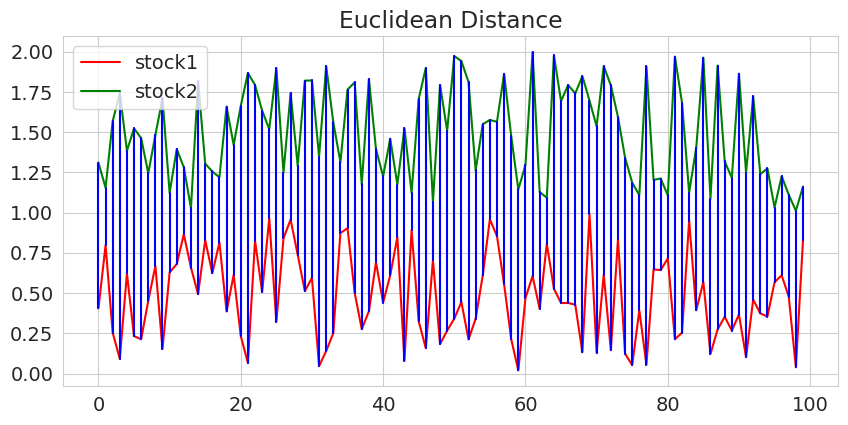
\includegraphics[width=10cm]{img/eculidian-sample.png} 
\caption{Standard Euclidean distance correlation using synthetic example}
\label{fig:euclidean_synth}
\end{figure}

Unlike Euclidean distances, DTW is a time-series analysis technique which is particularly suited to dealing with data that may be non-linear, have different speeds, or contain sequences that might align better with a certain amount of stretching or compression along the time axis. For our use case, this feature is important in ensuring that we capture trends more holistically, remaining agnostic of industries and time windows.

\begin{figure}[H]
\centering
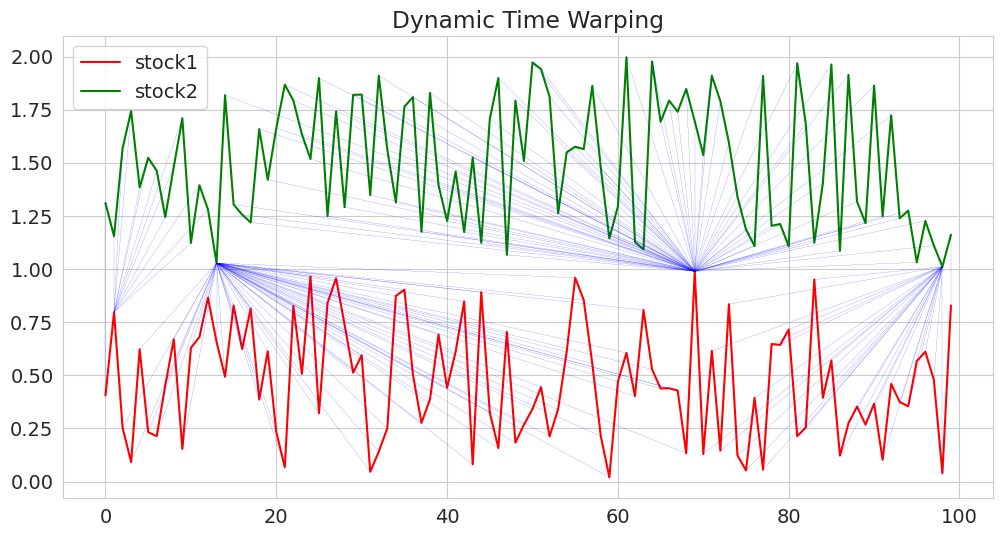
\includegraphics[width=10cm]{img/dtw-sample.png} 
\caption{Dynamic Time Warping using synthetic example}

\end{figure}

What can be observed above is that we are enabled to correlate points in \textit{stock1} to multiple other points in \textit{stock2} across the selected time window, in comparison to a direct point-to-point correlation based on the exact point in time in the Euclidean world (Fig. \ref{fig:euclidean_synth}).

In essence, DTW finds the optimal alignment between time-series by warping the time dimension in a way that minimises the overall distance between the series. Using DTW, we consider the temporal dynamics of stock price movements, providing a richer and more informative characterisation of stock behaviours than what might be derived from static per-stock metrics such as average return or volatility. 

Our application of the algorithm involved first computing a pairwise distance matrix between all stocks based on their DTW distance. This matrix was then used as the basis for clustering, with the goal of grouping together stocks that showed similar price movement patterns over time. The clustering was performed using several different techniques, including DTW Flat Clusters from Hierarchical Clustering and the K-Means algorithm. The relative performance of these techniques was then measured and compared using a variety of evaluation metrics, including the Silhouette score, the Davies-Bouldin index, the Calinski-Harabasz index, and visual assessment.

This application of DTW for stock clustering offered a more sophisticated approach to understanding stock market dynamics, which has the potential to inform more effective investment strategies. The results obtained were compared with those of traditional methods to evaluate the effectiveness of capturing complex patterns in stock market data: 


\begin{figure}[H] 
\centering
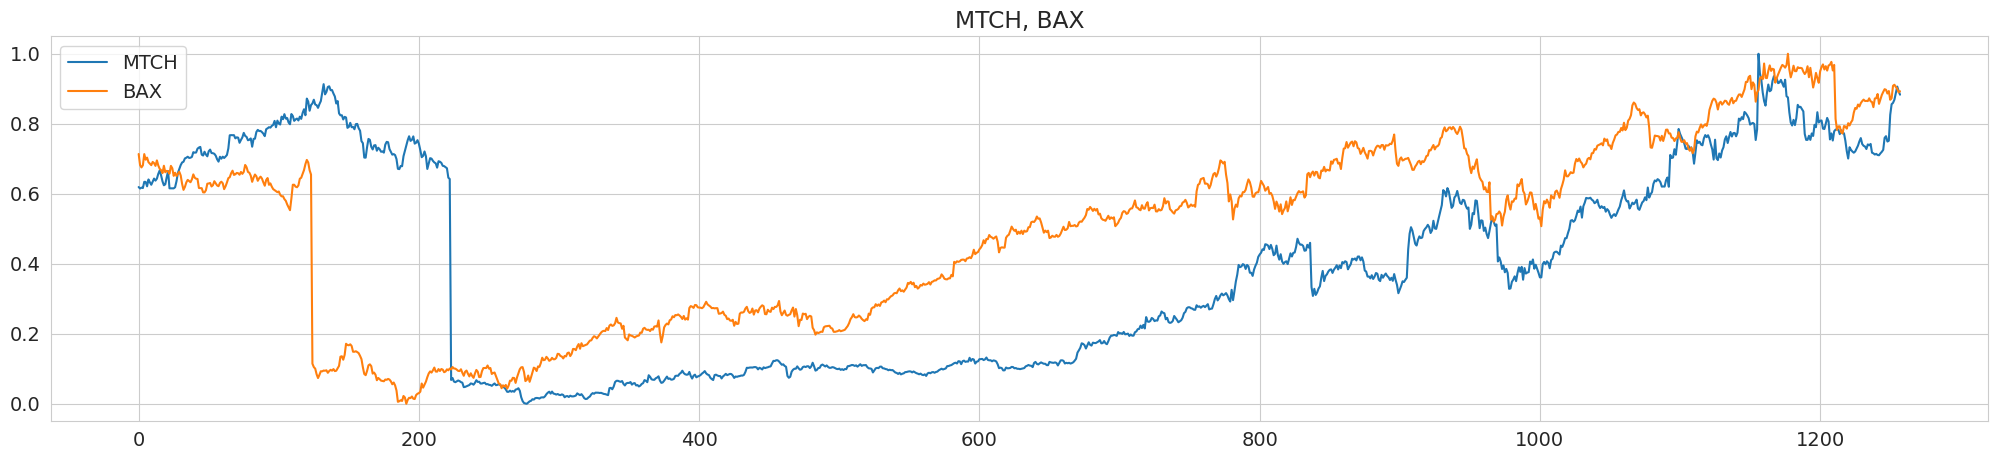
\includegraphics[width=12cm]{img/mtch-bax.png} 
\caption{Price time-series for MTCH and BAX stocks}
\label{fig:mtch-bax}
\end{figure}

In the figure above, we have a real-world example of two stocks behaving similarly at different points in time. MTCH is an Internet and Technology company while BAX is a Healthcare one, showcasing how interesting and diverse the clusters we generate can be. Our goal is to obtain similar results across a variety of stocks in different industries on our entire data-set. 

\subsection{Self-Organising Maps}

 SOM is an unsupervised neural network technique primarily used for visualising and summarising high dimensional data, influenced by the architecture of natural neural systems \cite{somBackground}.

 Compared to DTW, which cross-aligns sequences in a non-linear fashion, MiniSom creates a relational map between clusters as it groups data points into those clusters. The closer points are on the map, the more closely related they are to each other. 
 
 Furthermore, unlike Principal Component Analysis (PCA) which linearly reduces dimensions, SOMs can also deal with a high number of dimensions and capture non-linear relationships \cite{pcaSom}. In the case of stock data, which is non-linear by nature, we used SOMs as an alternative option to see what insights it could uncover compared to our other algorithms.

  It is important to note that with our decision to focus solely on closing price, we did not take advantage of SOM's ability to boil down high-dimensional data to fewer dimensions. However, as we will see in later sections, we have found SOM to be one of the best at clustering methods for our stock data, even with just one dimension. 
  
  In a future iteration of this experiment, we would propose leveraging data for other features such as trading volume to uncover more insights using Self-Organising Maps, for its ability to integrate more dimensions makes it future-proof and ready to use for the financial analyst.

 
\subsection{Evaluating}
\subsubsection{Silhouette Score}
We leveraged the Silhouette scoring technique proposed by Peter J. Rousseeuw \cite{silhouettes} in 1987 to measure how close each stock in a given cluster is to the samples in the neighbouring ones. Its numerical value ranges between [-1, 1], where the highest value indicates that the node is well-fit to its assigned cluster and would be poorly matched to neighbouring clusters. If most of the nodes have a value showing a good match, then the clustering configuration generated by the algorithm is better than one with fewer nodes having a high value. If many points have a low value, then the clustering algorithm may have generated either too many or too few clusters, or the effectiveness of assigning nodes to clusters has room for improvement.

The Silhouette score \( Silhouette(i) \) for a node \( i \) can be mathematically represented as follows:

\begin{figure}[H]
\centering
\begin{equation*}
Silhouette(i) = \frac{SmallestOuterAverage(i) - AverageWithinCluster(i)}{\max\{AverageWithinCluster(i), SmallestOuterAverage(i)\}}
\end{equation*}
\end{figure}

Where \( a(i) \) is the average distance from the \( i^{th} \) point to the other points in the same cluster and \(SmallestOuterAverage(i) \) is the smallest average distance from the \( i^{th} \) point to the points in a different cluster, minimised over all clusters.

To calculate the overall Silhouette score, that we want to maximise, for the data-set we can compute the average Silhouette score of all nodes as follows:

\begin{equation*}
SilhouetteOverall = \frac{1}{N} \sum_{i=1}^{N} Silhouette(i)
\end{equation*}

For our particular needs, we used Scikit-learn's implementation \cite{scikit} of the score as a metric to measure similarly behaving stocks, where each cluster represents a group of such stocks. As we are exploring the use of not only Euclidean distances but also Dynamic Time Warping, we will adapt the distance used to calculate the score per algorithm to leverage DTW distances where the algorithm is DTW in scope.

\subsubsection{Calinski-Harabasz Index}

Also known by the name of Variance Ratio Criterion (VRC), this metric was first introduced by Tadeusz Caliński and Harabasz JA in 1974 \cite{calinski}. It is composed out of the ratio of the sum of between-cluster dispersion and of inter-cluster dispersion for all nodes. We define dispersion as the sum of distances squared. 

For evaluation purposes, the higher the Calinski-Harabasz (CH) index value, the better the implemented clustering solution is considered to be. A higher value tells us, through the nature of the values that compose the formula, that the cluster is dense and well separated from other clusters, which makes it a good candidate for identifying stocks with similar behaviours. A higher value indicates better clustering since it means that the clusters are compact (low within-cluster dispersion) and well-separated (high between-cluster dispersion).

\begin{equation*}
\text{CH}(K) = \frac{\text{Trace}(B_K)}{\text{Trace}(W_K)} \times \frac{N - K}{K - 1}
\end{equation*}

\begin{itemize}
    \item \( B_K \) is the between-group dispersion matrix.
    \item \( W_K \) is the within-cluster dispersion matrix.
    \item \( N \) is the total number of samples.
    \item \( K \) is the number of clusters.
    \item \text{Trace} represents the sum of the diagonal elements, representing the sum of variances for each cluster.
\end{itemize}

The index provides a trade-off between the number of clusters and the clustering quality. 

In practical applications like stock market analysis, we used the Calinski-Harabasz index to determine the optimal number of clusters for algorithms like K-Means, where the number of clusters K needs to be specified as an input. By running K-Means with different K values and computing the index for each one, we selected the K that maximises the index, aiming also for visually well-defined and separated stock behaviour clusters.

\begin{figure}[H] 
\centering
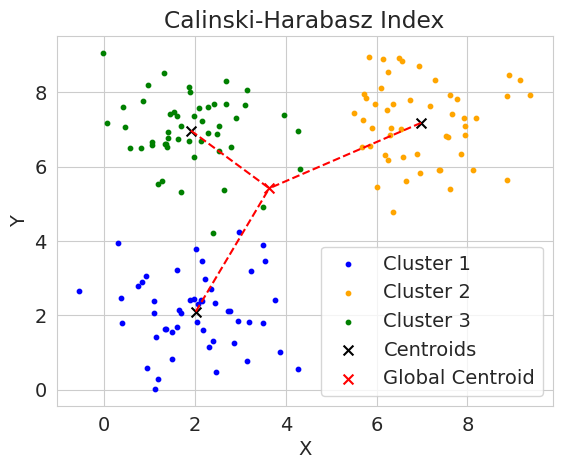
\includegraphics[width=10cm]{img/ch.png} 
\caption{Calinski-Harabasz centroids on a synthetic example}
\label{fig:ch}
\end{figure}

For every point, we measure its distance from the centroid of its cluster, where the centroid is the average position of all points in the cluster. The dispersion within a cluster is essentially the sum of the squared distances of all points in that cluster from its centroid.
The sum of the dispersions of all clusters gives the total within-cluster dispersion (W).

We then calculated the distance between the centroids of these clusters and the global centroid of the entire data-set. The between-cluster dispersion (B) is the sum of the squared distances of the centroids of all clusters from the global centroid, weighted by the number of points in the clusters.

For our use case, we included the CH index as an alternative to the Silhouette score to have an additional means of checking stock similarities and to have a point of comparison. 

\subsubsection{Davies-Bouldin Index}

The Davies-Bouldin index is another metric used to evaluate the quality of clusters created by a clustering algorithm representing the average similarity between clusters. It was originally proposed by David L. Davies and Donald W. Bouldin as a cluster separation methodology \cite{davies}. 

In this algorithm, we define similarity as a measure that compares the distance between clusters along with the size of the clusters themselves. The DB index ranges in value from 0 to infinity.

Unlike the Calinski-Harabasz index, which aims to be maximised, the Davies-Bouldin index has to be minimised to determine optimal clustering. We interpret values closer to zero as an indication of a better partitioning of stocks. A lower index means that clusters are compact (low intra-cluster distance) and well-separated from other clusters (high inter-cluster distance). 

\begin{equation*}
DB = \frac{1}{K} \sum_{i=1}^{K} \max_{i \neq j} \left( \frac{s_i + s_j}{d_{ij}} \right)
\end{equation*}

\begin{itemize}
    \item \( s_i \) is the average distance of all points in cluster \( i \) to the centroid of cluster \( i \).
    \item \( s_j \) is the average distance of all points in cluster \( j \) to the centroid of cluster \( j \).
    \item \( d_{ij} \) is the distance between centroids of clusters \( i \) and \( j \).
    \item \( K \) represents the number of clusters.
\end{itemize}

Similar to the Calinski-Harabasz index, the Davies-Bouldin Index is often used to determine the optimal number of clusters by comparing the index value given different numbers of clusters. This made the algorithm a great alternative to the two scoring algorithms above and provided us with another point of comparison for identifying stocks with similar behaviours. 

\subsubsection{Visual Inspection}
\label{sec:visual_inspection}

Whilst we have established mathematical metrics, we can also visually inspect how tight each cluster appears to be (intra-cluster similarity) and how distinct they are from each other (inter-cluster dissimilarity). 

We plotted each cluster's centroid against every stock in a cluster to visualise how similar the trends that have been grouped together were.

After applying a clustering algorithm to stock data, we plotted the time-series of each stock that belongs to the cluster in the same graph. For example, all stocks in \textit{Cluster 1} would be in one plot, those in \textit{Cluster 2} in another, and so on, exemplified in the following figure:

\begin{figure}[H] 
\centering
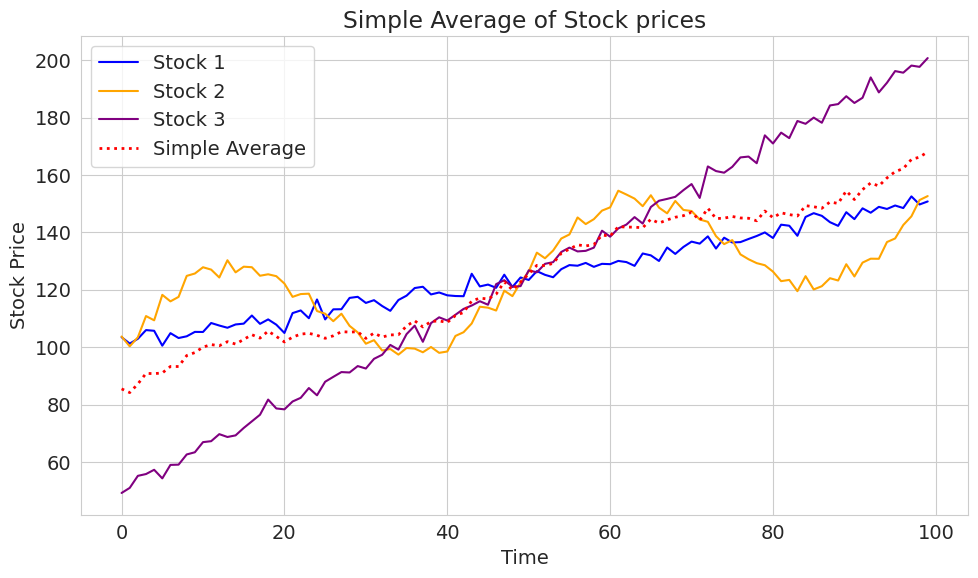
\includegraphics[width=10cm]{img/simple-average.png} 
\caption{Simple averaging of three synthetic stocks}
\label{fig:simple-average}
\end{figure}

An initial approach was by drawing an average line as is the case in Fig. \ref{fig:simple-average}. This was especially useful due to how complex it can be to assess the outcome of clustering with DTW using our selected metrics. For instance, if the clustering algorithm uses centroids (such as K-Means), these can also be overlaid on the cluster plots for comparison. 

A useful clustering will show a clear separation between different clusters. This separation can be observed visually, with each cluster plotting as a distinct \textit{bundle} of time-series lines.

Visual inspection allowed for a more intuitive, albeit subjective, understanding of the data, which can sometimes capture subtleties that quantitative metrics may overlook. In our application, we have noticed scenarios where the quantitative metrics suggested inadequate clustering, but visualising the outcome proved the opposite.

The major downside of visual inspection is its subjectivity. What looks like a distinct, well-separated cluster to one person might not to another. As the number of clusters or the complexity of the data grows, visual inspection becomes less practical with diminishing returns.

This method is more qualitative and may not provide the mathematical rigour needed for some applications, but we have used it because assessing the quality of DTW-based clusters would otherwise be too complex. 

\subsubsection{Visual Inspection with DTW Barycenter Averaging (DBA)}

In the case of DTW, we considered generating a DTW-averaged series for each cluster as a representative \textit{centroid}. In our use case, to enhance our ability to visually reason about the results generated in a DTW context, we made use of DTW Barycenter Averaging (DBA) as a technique used in Time-Series Analysis for calculating the centroid, or geometric centre, of a cluster of similar time-series shapes. This method exploits the potential of Dynamic Time Warping (DTW) to adjust for time shifts, especially since time-series data often has temporal shifts and non-linear changes in patterns. 

Traditional methods of computing average patterns, such as the arithmetic mean, may not capture these nuances effectively. To counteract this, the DBA method offered a more sophisticated approach that is not merely arithmetic by computing a \textit{barycenter}, a form of a weighted average, which serves as a representative shape for each cluster of time-series data.

This was achieved using the DTW method, which allowed a more flexible comparison of time-series by warping the time axis to align similar patterns. The \textit{barycenter} was computed in such a way that the total (DTW) distance between the \textit{barycenter} and the series in the cluster was minimised.

\begin{figure}[H] 
\centering
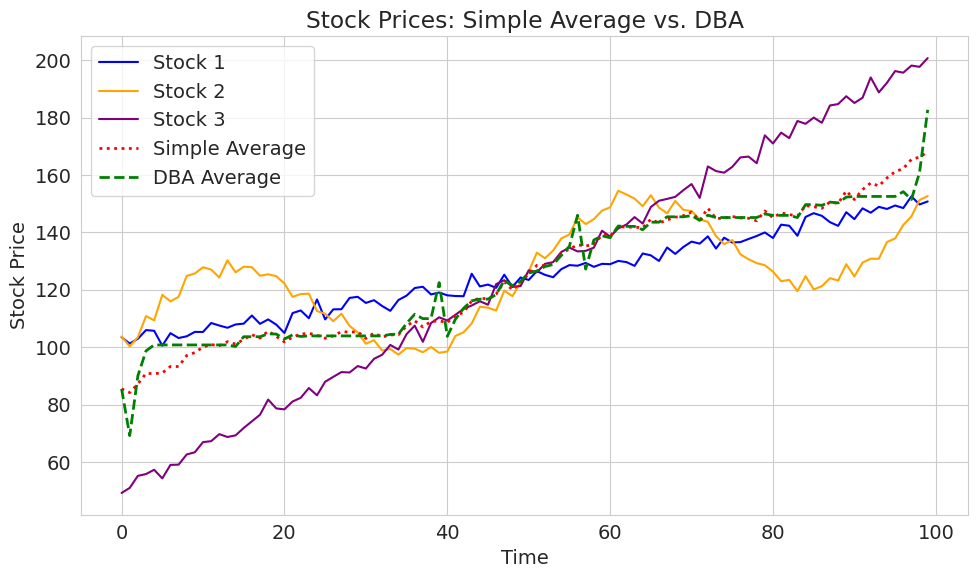
\includegraphics[width=10cm]{img/average-vs-dba.png} 
\caption{Averaging of three synthetic stocks alongside DBA}
\label{fig:average-vs-dba}
\end{figure}

In the figure above, we can see that the simple average (red dotted line) does not provide a good representative for the group of time-series. In places where the stocks diverge greatly, the simple average merely provides the arithmetic mean of these values.

For instance, in the case of our synthetic data, the simple average gets pulled in the direction of \textit{Stock 2} during its sinusoidal peaks and valleys, but does not capture the essence of \textit{Stock 1} or the trend of \textit{Stock 3} at all. In other words, the representation could be described as \textit{sitting on the fence} (neither here nor there), which might not be the best representation for any of the stocks.

DBA (green dashed line) works differently. Instead of taking a point-wise arithmetic mean, it attempts to find a sequence that minimises the DTW distance to all sequences in the data-set.

Even with our set of synthetic stocks in Fig. \ref{fig:average-vs-dba} above, the DBA captures the overall trend far better than the simple average. It does not just follow the peaks and dips of \textit{Stock 2}, instead providing a middle ground that, while not matching any individual stock perfectly, is a more balanced representative of the set. This showcases DBA's ability to generate a central time-series that takes into account the dynamics and captures the patterns of all time-series in the set.

In the context of clustering, DTW and DBA provide a powerful tool for the formation of meaningful clusters of time-series data and their representative shapes, irrespective of the inherent time shifts within the cluster. This process enables the capturing of characteristic patterns within the cluster, providing essential insights into the data.

We visually gauged how similar the stocks in each cluster were over time, especially after DTW alignment. A good cluster will have stock time-series that are closely aligned, which will be evident in the plot.

\section{Analysis and Discussion}

\subsection{Overview}

We have focused on companies recognised by the market as being of value through index constituency, and for which we were able to extract over 5 years of data, with over 2000 observations (individual daily stock prices). This ensured that we were able to base our analysis using companies with a consistently substantial amount of data points. 

In this section, we present an in-depth exploration of this data-set and apply the algorithms we have presented previously. We aimed to form 23 clusters with each data-set (the square root of the total number of stocks), record the metrics we have settled on and visually analyse the resulting clusters. At the end of this section, we will look holistically at the results and present conclusions that have surfaced.

\subsection{Exploratory Analysis}

\subsubsection{Company Profiles}

We have focused on S\&P 500 and NASDAQ 100 companies covering multiple industries, but it is worth noting that the data is biased towards US companies due to their large presence in these indices, as we will explore later on.

Our analysis encompassed a total of 521 distinct companies, after cleaning up the duplicates in the combination of the two considered indices: S\&P 500 and NASDAQ 100. However, due to insufficient data across a suitable time window for all series, we have decided to omit 30 companies from our study (27 US, 1 IT, 1 AU, 1 CN), which results in the following distribution over countries: 

\begin{table}[H]
\centering
\begin{tabular}{|c|c|c|c|c|c|}
\hline
\textbf{Country} & \textbf{\#} & \textbf{Country} & \textbf{\#} & \textbf{Country} & \textbf{\#} \\
\hline
US & 466 & IE & 10 & CH & 4 \\
GB & 4 & BM & 2 & NL & 2 \\
CN & 1 & CA & 1 & UY & 1 \\
\hline
\end{tabular}
\caption{Distribution of companies by country}
\label{tab:my_label}
\end{table}


As a result, our experiment was conducted with a final set of 491 companies distributed in 11 primary sectors as follows:


\begin{figure}[H]
\centering
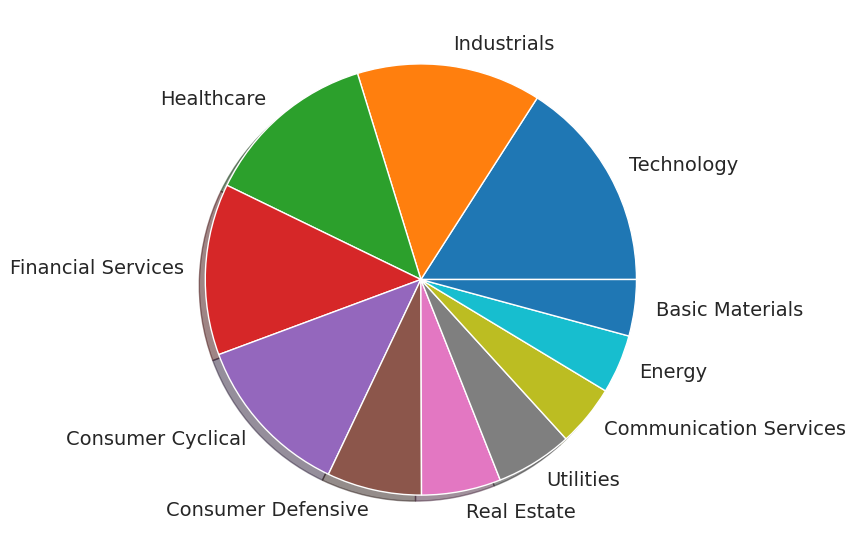
\includegraphics[width=10cm]{img/industries.png} 
\caption{Distribution of companies by their Sector}

\end{figure}

We can see below that there is a good cross-sector distribution of stocks, allowing us to put the algorithms we have chosen to a stress test. 

\begin{table}[H]
\centering
\fontsize{7}{7}\selectfont
\begin{tabular}{|c|c|c|c|c|c|}
\hline
\textbf{Sector} & \textbf{Count}  \\
\hline
Technology & 73 \\
Industrials & 69 \\
Financial Services & 66 \\
Healthcare & 65 \\
Consumer Cyclical & 59 \\
Consumer Defensive & 35 \\
Real Estate & 29 \\
Utilities & 29 \\
Communication Services & 23 \\
Energy & 23 \\
Basic Materials & 20 \\
\hline
\end{tabular}
\caption{Raw data for the distribution of companies by their Sector}
\label{tab:rawsector}
\end{table}



\subsubsection{Historical Stock Prices}

Our overall data from S\&P 500 and NASDAQ 100 companies covers stock prices from January 2015 to January 2023. We have selected the closing price for each day, as in the price the company traded at the close of the trading day, each day. We selected this variable as it is the price most often used in both academic and investment settings, being the focus of investors and fund evaluations alike \cite{closePrice}. 


\begin{figure}[H]
\centering
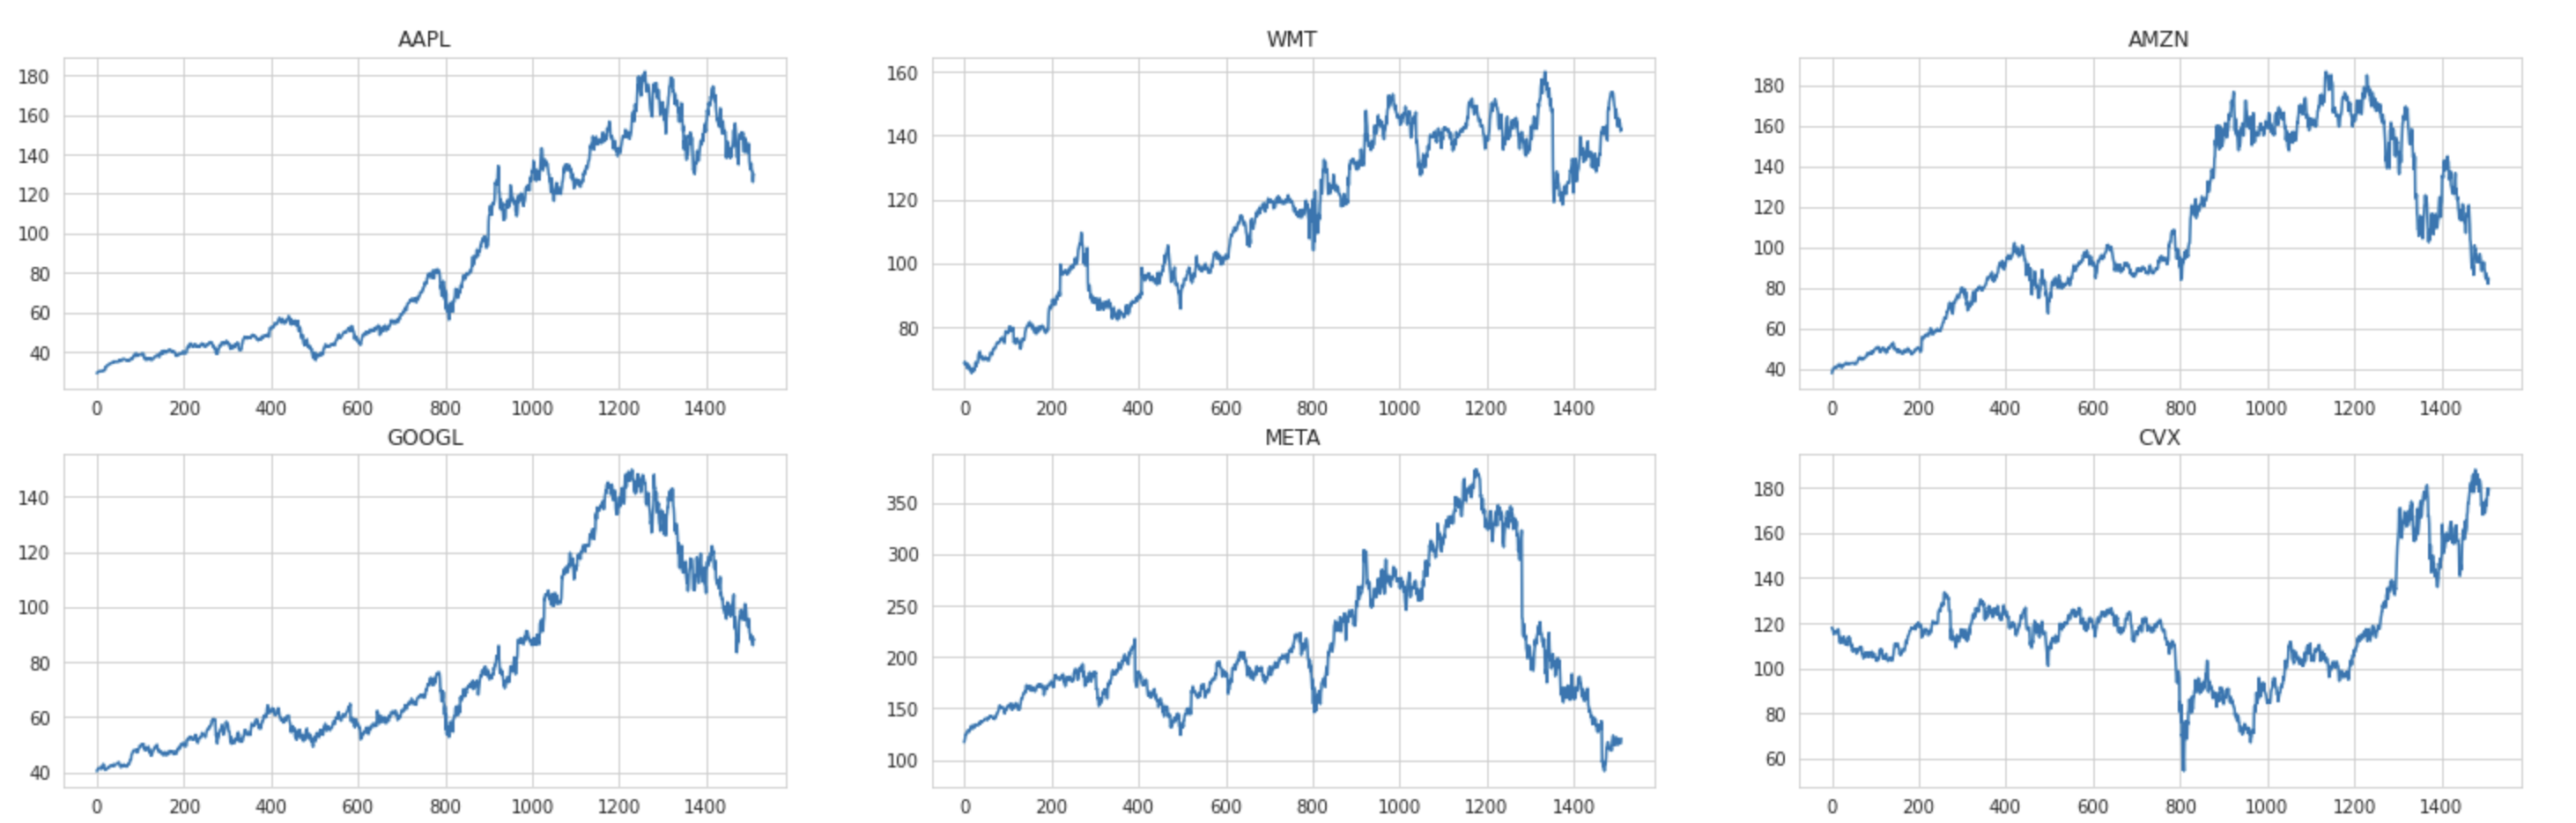
\includegraphics[width=12cm]{img/stocks.png} 
\caption{Sample of 6 entities in the stock data we have gathered}

\end{figure}

The above shows an example of the stock data we have gathered across the specified time frame and on which we have conducted our analysis further. 

To further understand our data, we generated a correlation matrix for a subset of 100 stocks using the Pearson correlation coefficient method from the \textit{Pandas} library. In the figure below, we can observe that a large number of stocks have a high correlation which is likely to make it difficult for well-distinguished clusters to be generated. This problem becomes apparent when we explore \textit{\hyperref[sec:stockskmeanseuclidean]{K-Means using Euclidean distance}} later on, with most stocks being assigned to a low number of clusters, further emphasising that we should take a varied approach in clustering the data:
 
\begin{figure}[H]
\centering
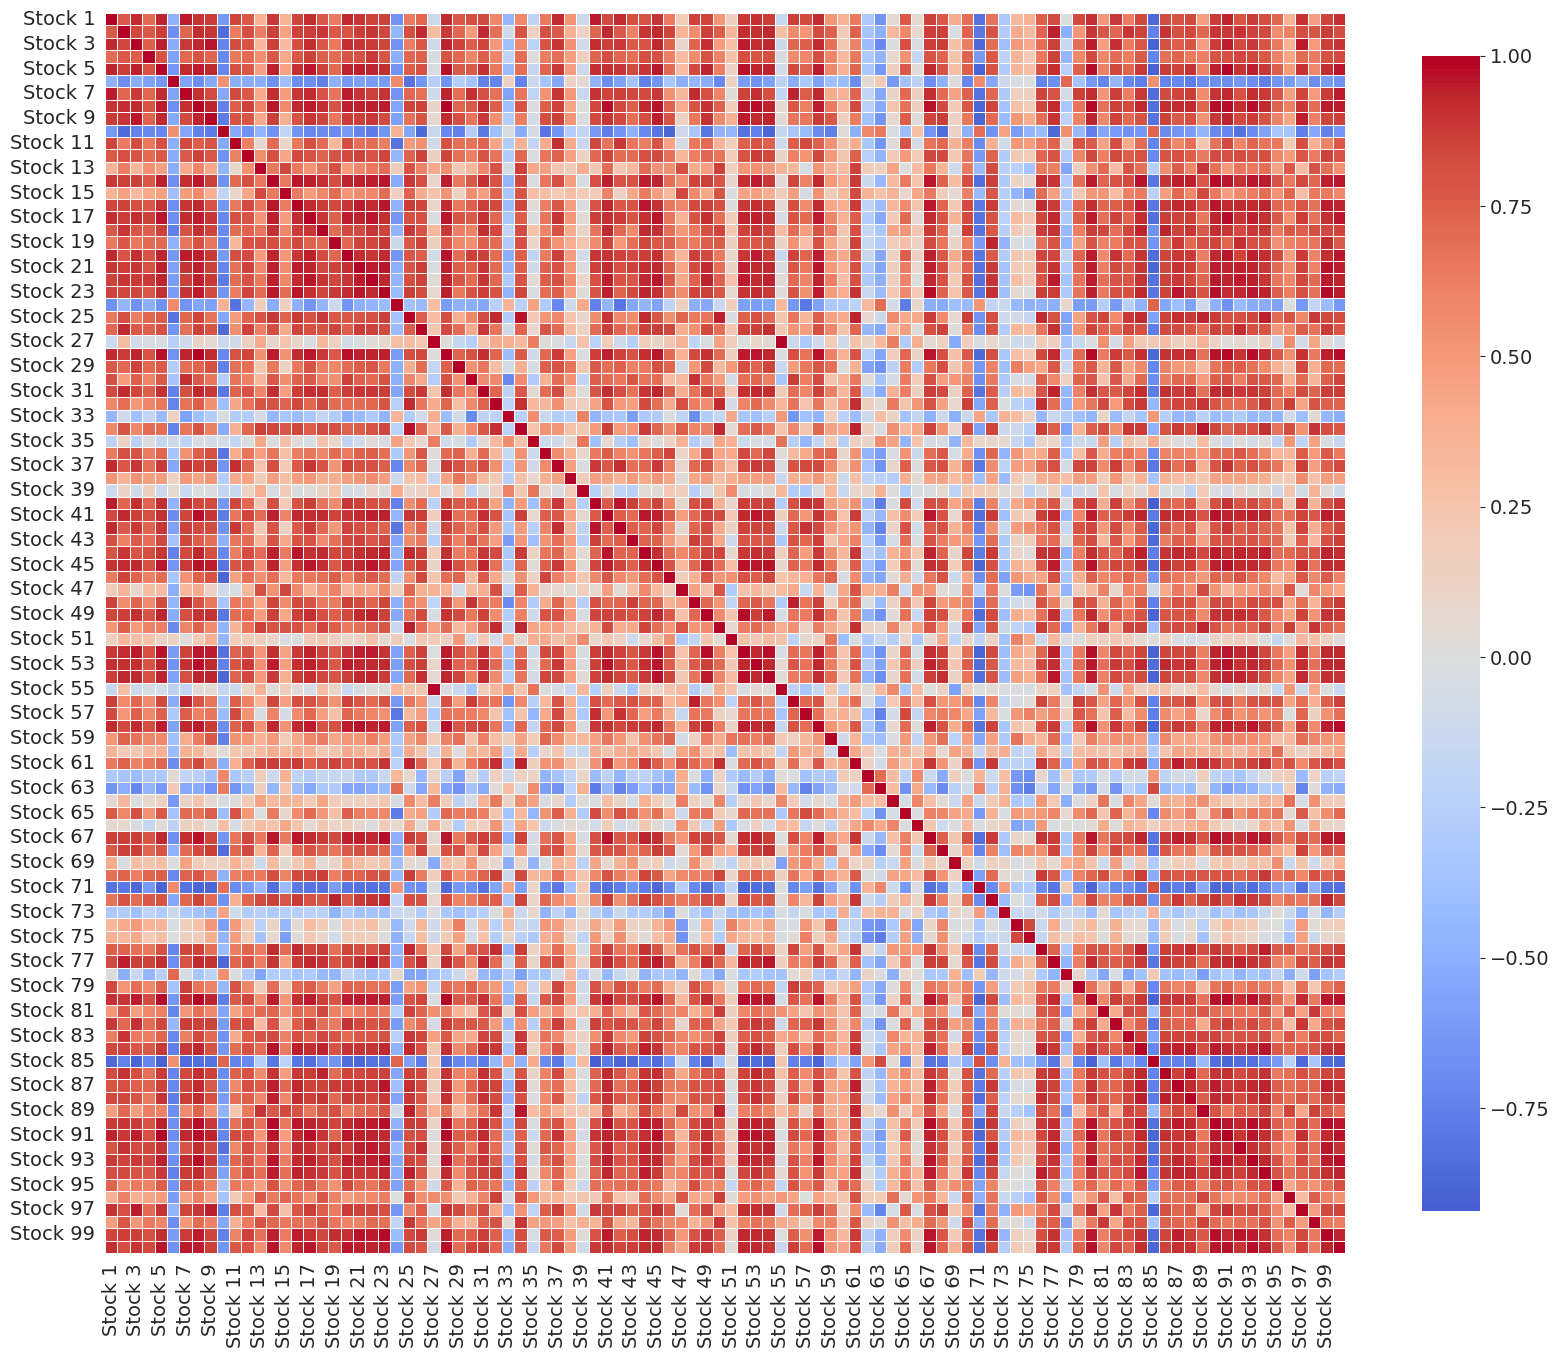
\includegraphics[width=10cm]{img/correlation.png} 
\caption{Correlation matrix for a subset of 100 stocks}
\end{figure}

\subsection{Pre-processing}

\subsubsection{Time-frame}

Although our overall data covers a range of 8 years, we decided to pick a smaller time range to ensure consistency of data availability across all stocks. Using the below algorithm, we converged on a window of time spanning from the 1st of January 2017 to the 1st of January 2020.

\begin{figure}[H]
\centering

\begin{lstlisting}
min_start = '2017-01-01'
max_end = '2020-01-01'

for prices in stock_prices:
  if len(prices) > 2000:
    min_start = max(prices.index[0], min_start)
    max_end = min(prices.index[-1], max_end)
\end{lstlisting}
\caption{Algorithm for converting on the time-window}
\end{figure}

The reason for selecting this specific window of time was to avoid having the data biased by the COVID-19 pandemic \cite{covidMarkets} \cite{globalCovid}. Another consideration for selecting this specific time window was ensuring we had pricing historical data points for all the companies selected from our data-set, and guaranteed at least 2000 observations per company.


\subsubsection{Normalisation}

With DTW, SOM and K-Means, our goal was to compare stocks with similar trend lines across time. In other words, we were looking for similar \textit{shapes}.

However, none of the algorithms are invariant to scale, which means that the distance between time-series does depend on the magnitude of their values. Thus, if we have two time-series that are identical in shape but have different magnitudes, the algorithms will incorrectly measure a greater distance between them than if they had the same magnitudes. 

To further emphasise the impact for our use case of clustering stocks, we needed to consider that stock prices can vary wildly between companies, as some companies can trade at \$300 per share while others at \$9. This can lead to time-series with different magnitudes being clustered together, even if they are not very similar in shape. 

\begin{figure}[H]
\centering
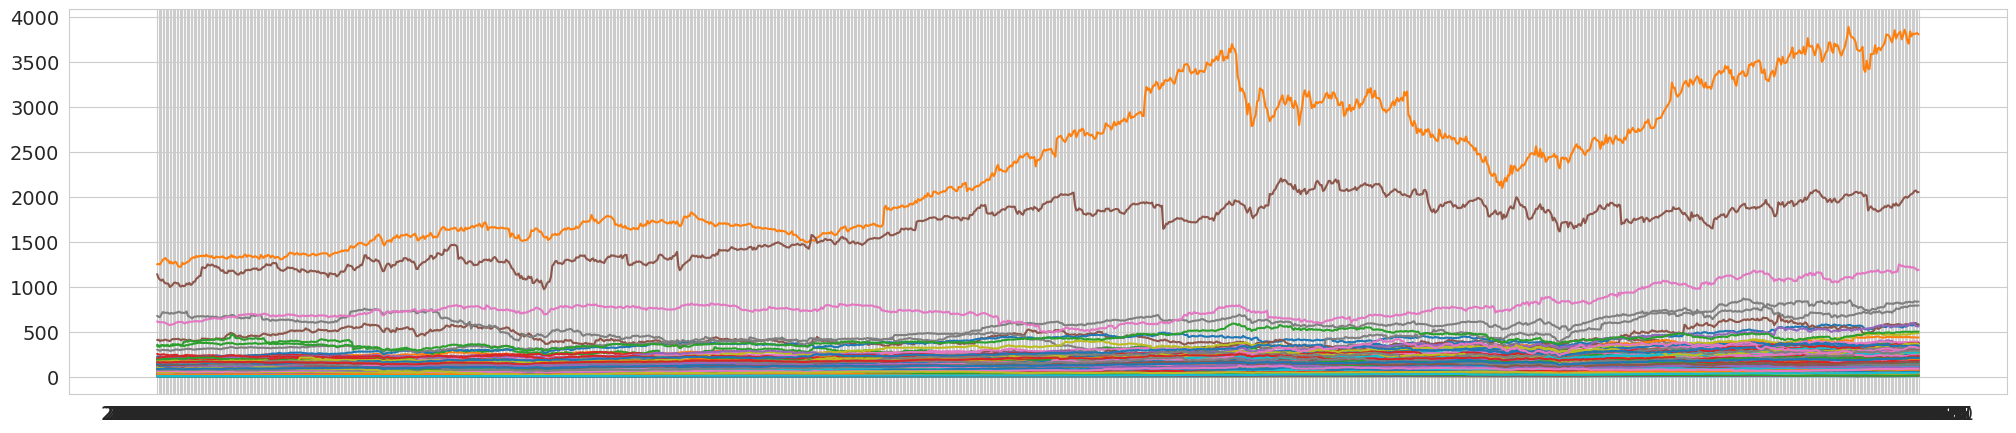
\includegraphics[width=12cm]{img/all-stocks.png} 
\caption{All stocks in the data-set at scale before normalisation}
\label{fig:prenorm}
\end{figure}

In the figure above we can observe how a limited number of stocks which are high in their price-point flatten all others which are on the lower end of the spectrum, resulting in 5 stocks overtaking the other 424 entries. Normalisation can help to address this problem by making all of the time-series in the data-set be at the same scale. 

There are a number of different ways to normalise time-series data. One common approach to normalisation, which we have employed, is to min-max scale the data, which involves subtracting the minimum value from each time-series and then dividing by the range of values: 

\begin{figure}[H]
\centering

\begin{lstlisting}[language=Python]
from sklearn.preprocessing import MinMaxScaler

def normalize_stock_prices(stock_prices):
    """
    Normalize stock prices using MinMaxScaler.

    Parameters:
    - stock_prices: List of stock price arrays.

    Returns:
    - normalized_prices: List of normalized stock price arrays.
    """
    normalized_prices = []
    scaler = MinMaxScaler()

    for prices in stock_prices:
        normalized = scaler.fit_transform(prices.reshape(-1, 1))
        normalized_prices.append(normalized.flatten())

    return normalized_prices

normalized_stock_prices = normalize_stock_prices(stock_prices)
\end{lstlisting}

\caption{Algorithm for normalising our data with a MinMaxScaler}
\end{figure}

This ensures that all of the time-series have values between 0 and 1, making patterns significantly more recognisable:

\begin{figure}[H]
\centering
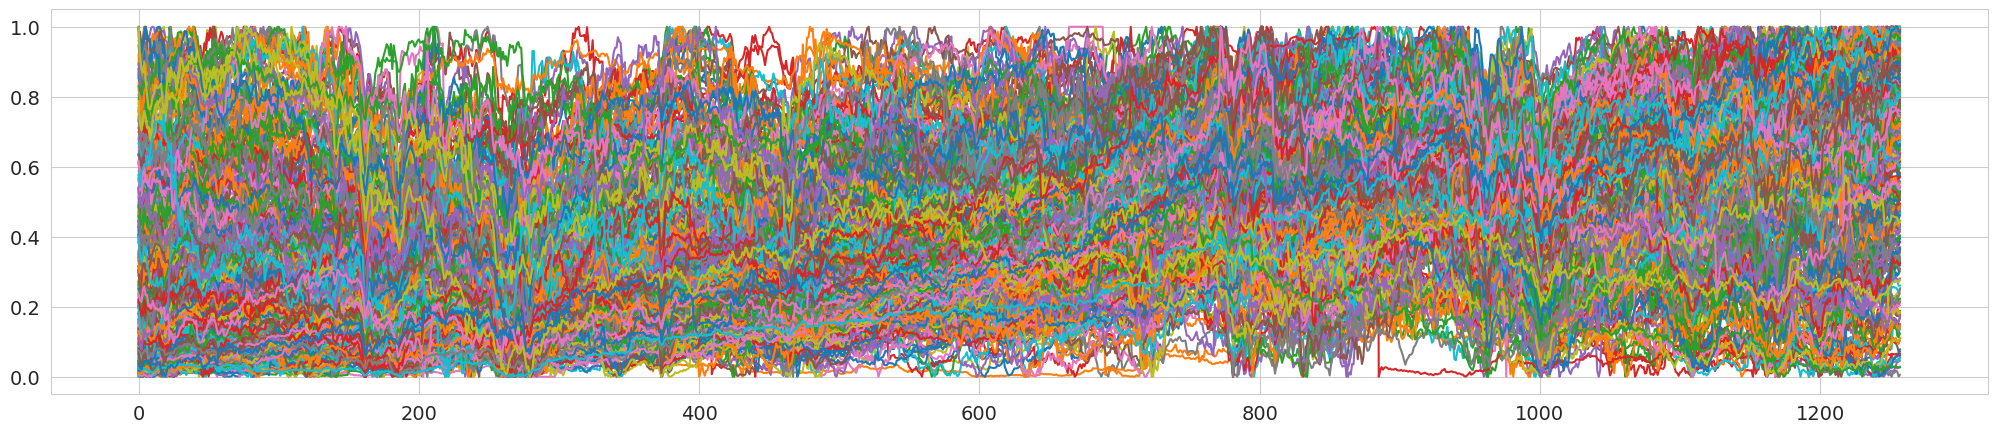
\includegraphics[width=12cm]{img/all-stocks-normal.png} 
\caption{All stocks in the data-set normalised}
\label{fig:normal}
\end{figure}

Post-normalisation, all of our stock data fell within a consistent range [0-1], without any one stock series overtaking the others simply through their high price, visually represented in the figure above, compared to Fig \ref{fig:prenorm}. It was on this normalised data that we were then able to use clustering algorithms. 

Normalisation gives us the certainty that we are comparing the stocks based on their relative performance rather than absolute values, which can be especially useful for stocks across different sectors and pricing scales.

\subsection{K-Means Euclidean}

\subsubsection{Overview}

The purpose of considering the K-Means Euclidean algorithm was to create a point of reference to benchmark the Dynamic Time Warping based methodologies. Having explained the difference between Euclidean and DTW in the \textit{\hyperref[sec:dtw]{Dynamic Time Warping Clustering}} section, we will now look at the findings we have observed when applying Euclidean K-Means clustering.

\subsubsection{Algorithm}

K-Means clustering is a type of unsupervised learning algorithm used to partition a set of points into a number, K, of clusters, where each point belongs to the cluster with the nearest centroid. The distance measure often used in K-Means is Euclidean distance. The algorithm tries to minimise the variance within each cluster and maximise the variance between clusters as follows:

\begin{itemize}
    \item K initial centroids are randomly selected.
    \item Each point in the data-set is assigned to the nearest centroid, and it becomes a member of that cluster.
    \item The centroids are re-calculated as the mean of all points in the cluster.
    \item Steps 2 and 3 are repeated until the centroids no longer change significantly. 
\end{itemize}

K-Means can be applied to stock market analysis in several ways:

\begin{itemize}
    \item To classify similar stock price behaviours.
    \item To identify patterns, anomalies, or trends in the market.
    \item To create portfolios of stocks that behave similarly, aiming to diversify risks.
\end{itemize}

For the purposes of our use case, we have chosen to use this algorithm to create 23 clusters, using the square root of the 429 total stocks in our data as a generic rule of thumb, applying the three different scoring systems described above on them. 

The following figure shows the trend of our metrics depending on the number of clusters we generated using K-Means: 

\begin{figure}[H]
\centering
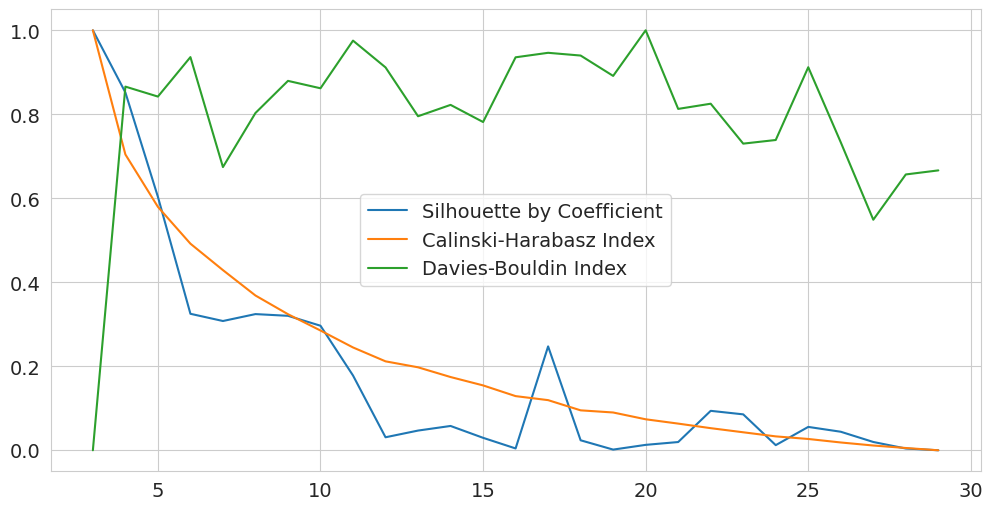
\includegraphics[width=8cm]{img/kmeans-index-comparison.png} 
\caption{Index comparison by number of clusters}
\label{fig:kmeansindex}
\end{figure}

In Fig. \ref{fig:kmeansindex} above we can see that the Silhouette score trends to 0 after 10 clusters are considered, which would signify the clusters are not well matched after that. The Calinski-Harabasz score, which we aim to be maximised, decreases linearly with the increased number of clusters. The Davies-Bouldin index, which aims to be minimised, is high for all clusters with more than 4 nodes.

This would perhaps suggest we should generate 4 clusters instead of 23. However, it can be observed in our findings that visually recognisable patterns have been identified within the noise and that the metrics are on the low side due to the large and very diverse data-set.

\subsubsection{Limitations}

The following are limitations of K-Means Euclidean that we subsequently tackled through the use of K-Means DTW, Flat Clusters from Hierarchical Clustering and MiniSom:

\begin{itemize}
    \item Euclidean distance is linear and may not capture non-linear relationships in stock price movements.
    \item Outliers or noises can heavily influence the clustering.
    \item The algorithm is sensitive to the initial selection of centroids.
    \item The number of clusters (K) has to be set implicitly rather than the best candidate is automatically derived by the algorithm.
    \item In cases where stocks are analysed across multiple dimensions (variables), Euclidean distance can suffer from the \textit{curse of dimensionality}.

      
\end{itemize}

\subsubsection{Application in Stocks}
\label{sec:stockskmeanseuclidean}

Running on our entire data-set of 491 stocks, we have done an initial configuration of the 23 clusters, which took 1 second to compile the model and generate clusters in our parallel computing environment, with 10 iterations allowed. 

\begin{figure}[H]
\centering
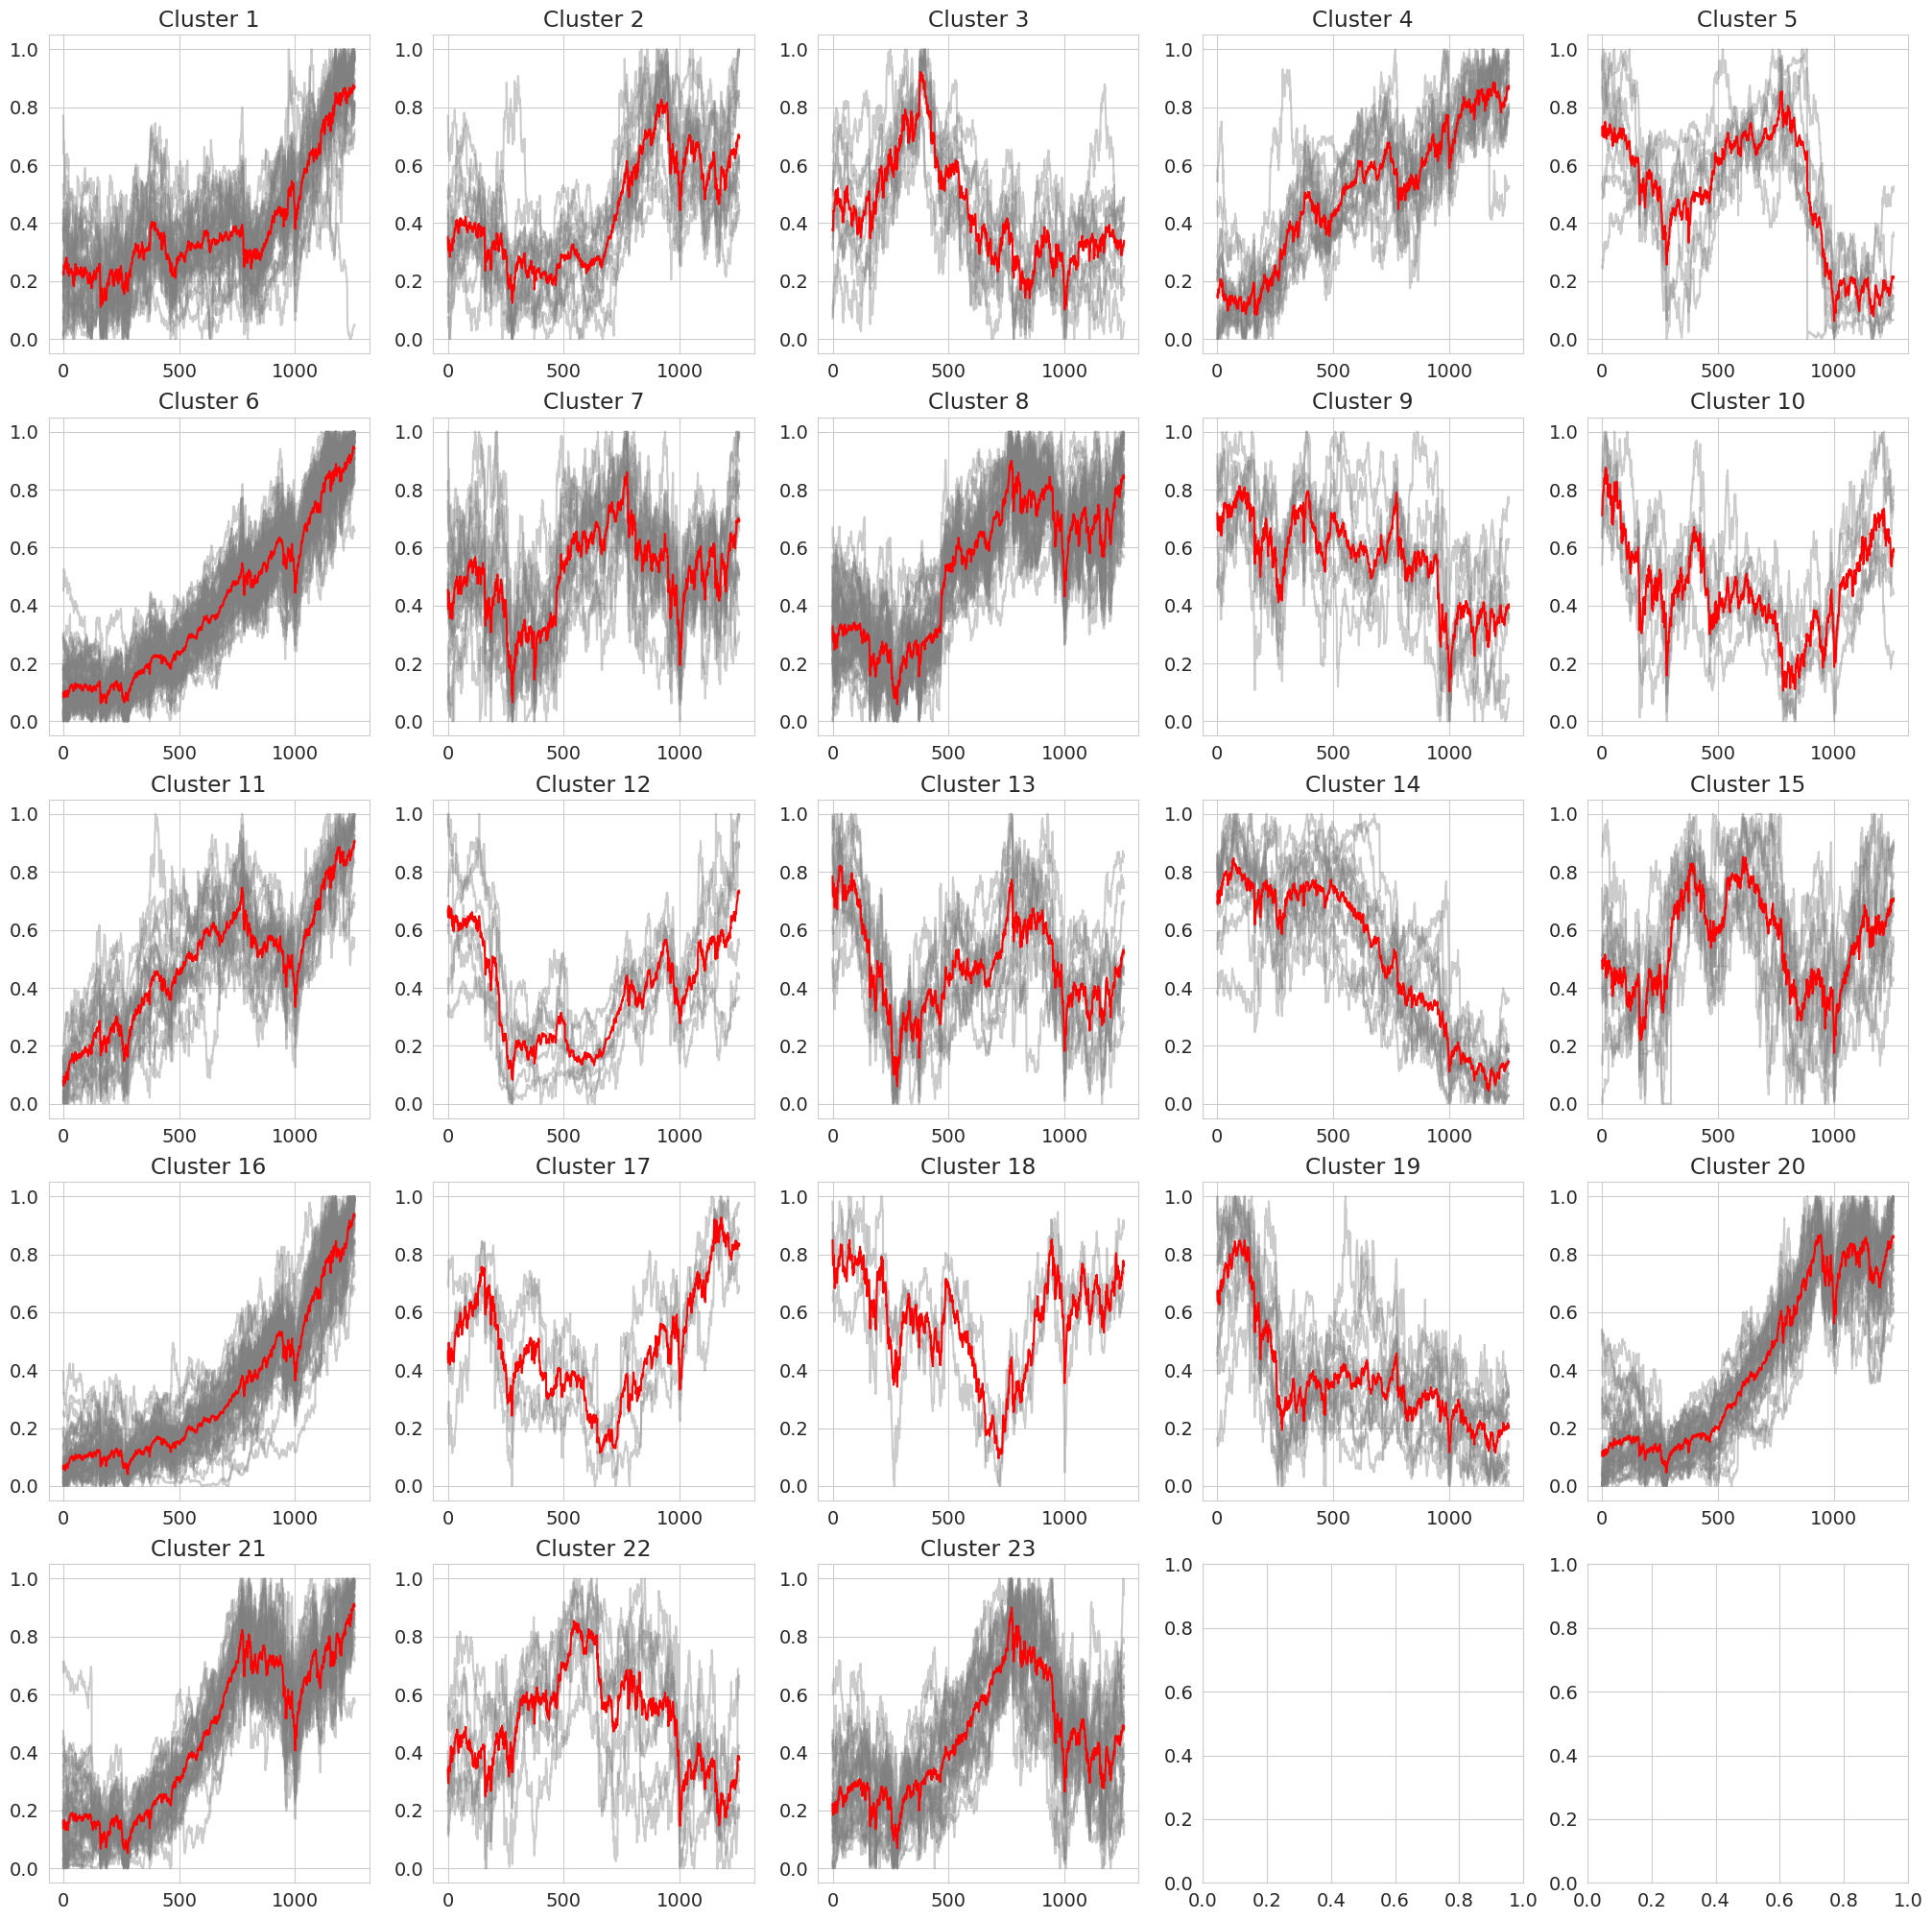
\includegraphics[width=12cm]{img/kmeans-euclidean-average.png} 
\caption{K-Means clusters overlaid with averaged centroid line}
\label{fig:kmeans_average}
\end{figure}

In Fig. \ref{fig:kmeans_average} above we can observe the 23 clusters generated, with an overlay of their averaged centroid line. We can distinguish that stocks were grouped in discernible patterns, with an obvious general trend to the stocks selected within each group. Some clusters such as \textit{Cluster 1} and \textit{Cluster 19} are more diverse and noisy, which would likely exclude them from consideration in an investment strategy, but \textit{Cluster 13} and \textit{Cluster 8} for example show very specific trends:

\begin{figure}[H]
\centering
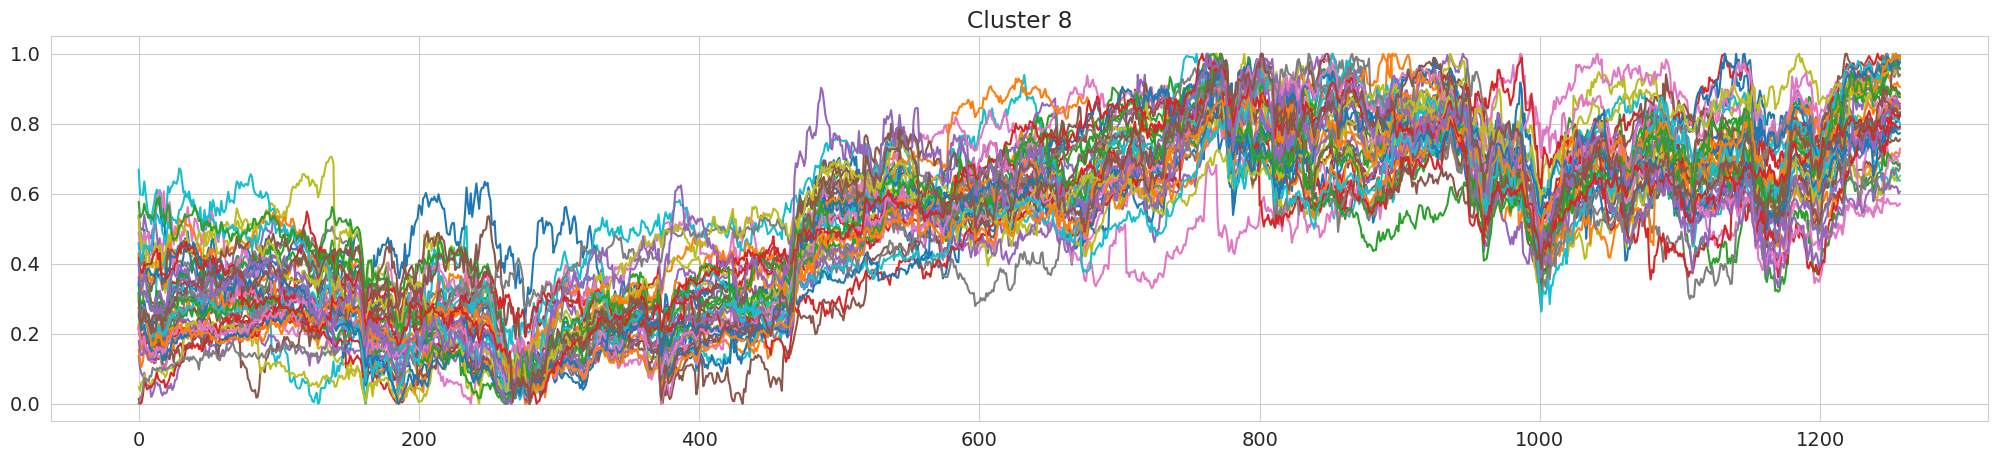
\includegraphics[width=12cm]{img/euclidean-cluster8.png} 
\caption{K-Means Euclidean - Cluster 8}
\label{fig:kmeans_c8}
\end{figure}

K-Means clustering scored as follows in our tracked metrics:
\begin{itemize}
    \item \textit{Silhouette score:} 0.109
    \item \textit{Calinski-Harabasz index:} 51.690
    \item \textit{Davies-Bouldin index:} 1.789
\end{itemize}

A comparison of these scores for all algorithms can be found in the \textit{\hyperref[sec:compare]{Scoring and Comparison}} section.

We also checked the distribution of stocks within their clusters:

\begin{figure}[H]
\centering
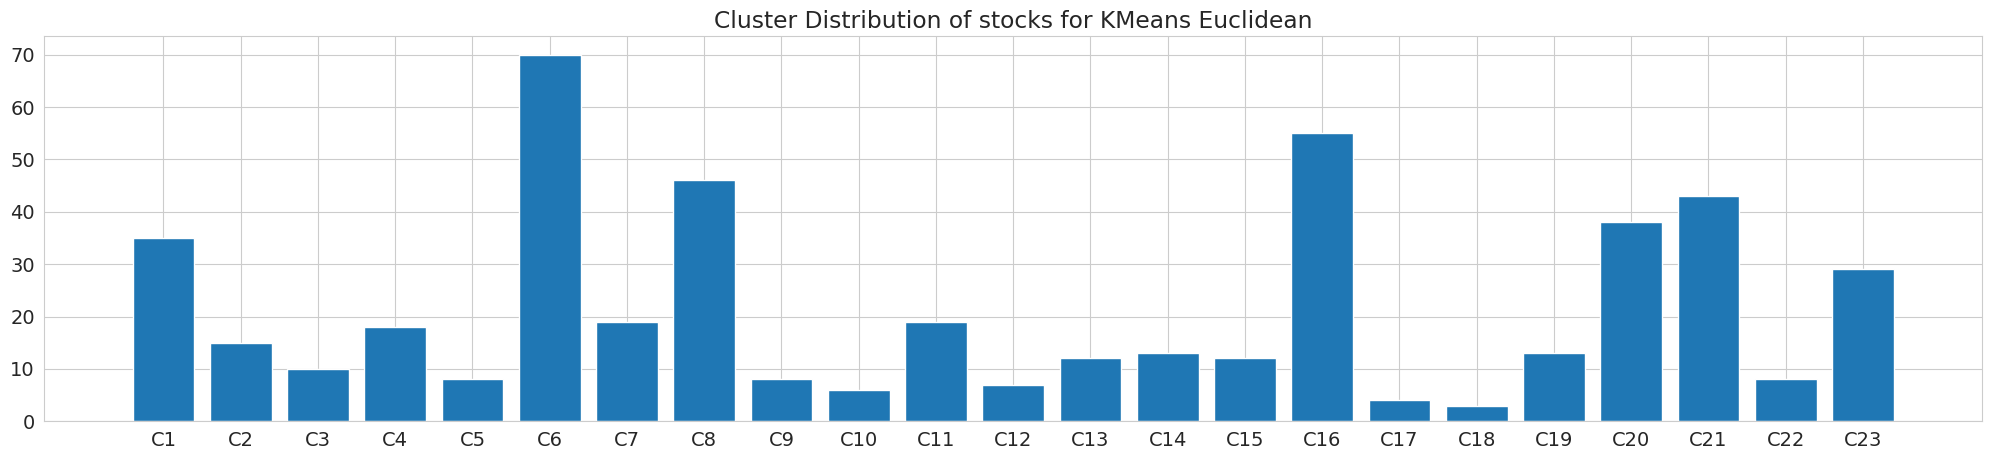
\includegraphics[width=12cm]{img/kmeans-euclidean-distrib.png} 
\caption{Distribution of stocks within their K-Means clusters}
\label{fig:euclidean_distrib}
\end{figure}

Approximately 70\% of clusters have more than 10 stocks, over multiple industries. We can observe that 7 of the clusters (\textit{C1}, \textit{C6}, \textit{C8}, \textit{C16}, \textit{C20}, \textit{C21}, \textit{C23}) contain most of the stocks, suggesting a bias or skew in the clustering. 

In both Fig. \ref{fig:kmeans_average} and Fig. \ref{fig:euclidean_distrib} we noticed numerous outliers in terms of clusters with a low number of stocks such as \textit{C5}, \textit{C19}, \textit{C17} and \textit{C18}. Further on, we will use this as a base of comparison with the results of other algorithms and find more uniform distributions.

\begin{figure}[H]
\centering
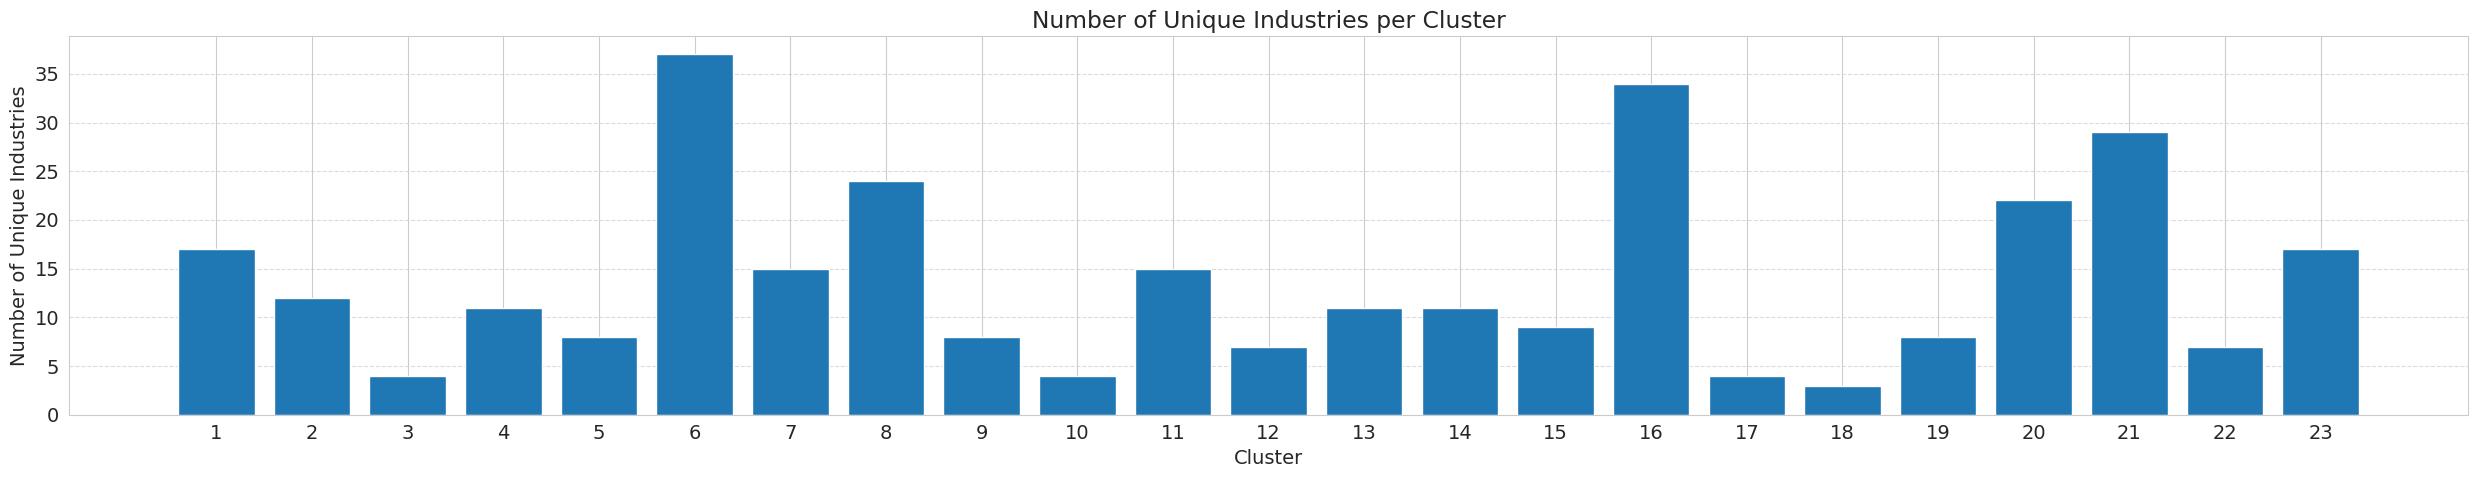
\includegraphics[width=12cm]{img/kmeans-industries.png} 
\caption{Distribution of industries in their K-Means clusters}
\label{fig:kmeans_industries}
\end{figure}

The distribution of industries in clusters gives us confirmation towards the fact that clustering algorithms can be leveraged to understand how we could connect multiple cross-industry stocks when designing a portfolio strategy.

We can also observe a direct proportionality relationship between the number of stocks and the number of industries in clusters.

\subsection{DTW Flat Clusters From Hierarchical Clustering}

\subsubsection{Overview}
We have described how Dynamic Time Warping (DTW) measures the similarity between two temporal sequences, having its primary utility stemming from its ability to find optimal alignment between two time-series that may not act similarly at specific points in time but might do so asynchronously.
 
For the findings in this section, we have computed a condensed distance matrix of DTW distances between all pairs of nodes, thus with a zeroed-out diagonal. This is very computationally expensive to generate for large data-sets, therefore we have parallelised the execution in Python.

 We then explored generating flat clusters from the resulting hierarchical clustering dendrogram using SciPy's \textit{fcluster} functionality. 

\subsubsection{Algorithm}

We generated our similarity DTW pairwise matrix by computing the DTW distance between all stocks in parallel and generating the \textit{Z} linkage that encodes a tree (dendrogram structure) representing the clustering process, leveraging the following Python approach:

\begin{figure}[H]
\centering
\begin{center}
\begin{lstlisting}[language=Python]
def compute_dtw(i, j):
  distance = dtw(stock_prices_normal[i], stock_prices_normal[j])
  return [[i, j], distance]

to_process = []
n = len(stock_prices_normal)  # Number of stocks
for i in range(n):
  for j in range(n):
    if i != j:
      to_process.append([i, j])

results = Parallel(n_jobs=-1)(delayed(compute_dtw)(x[0], x[1]) for x in to_process)

dtw_matrix = np.zeros((n, n))
for result in results:
  dtw_matrix[result[0][0], result[0][1]] = result[1]

condensed_dist_matrix = squareform(dtw_matrix)

Z = linkage(condensed_dist_matrix, method='ward')
\end{lstlisting}
\end{center}
\caption{Python algorithm for parallel DTW using Ward's minimum}
\end{figure}

In the next section, we will see the linkage dendrogram (Fig. \ref{fig:kernel_dendrogram}) by using Ward's minimum variance method which tries to minimise the variance of the distances between the clusters that are being merged.

Other options considered were: single (shortest distance between two points in a cluster), complete (maximum distance between two points in each cluster) and average (distance is defined as the average distance between every pair of points in the two clusters) linkage. For our stock series and DTW, Ward's minimum linkage was a more fruitful choice when visually analysing the outcome. Average might be a more intuitive natural choice for DTW since Ward uses Euclidean distances, but it generated significantly more clusters with individual single stocks regardless of the number of clusters which is not ideal. We will further explore the dendrograms visually in the next section. 

The follow-up last step was to generate flat hierarchical clusters using \textit{fcluster} with \textit{maxclust} as we want to specify exactly the number of clusters we want to generate:

\begin{lstlisting}
fcluster(Z, hierarchical_k, criterion='maxclust')
\end{lstlisting}

\subsubsection{Visualising Through Dendrograms}

To visualise our use of the DTW distance matrix and linkage generated, we used dendrograms. They are hierarchical tree diagrams that represent the hierarchical relationships calculated between stocks. In the context of time-series stock data processed using flat cluster methods, dendrograms become useful in:

\begin{itemize}
    \item Offering a visual representation of the nested hierarchy of time-series data clusters. The height in the dendrogram at which two clusters merge represents the distance at which they were joined, thus giving insights into the relative similarities between different clusters.
    
    \item Analysing the structure of the dendrogram, one can deduce an appropriate number of clusters for further analyses. Large jumps in merge heights can indicate relevant cluster structures.
    
    \item Scrutinising the branch lengths and heights of merges, through which one can infer the similarity between various clusters. Closer branches typically imply higher similarity.
    
    \item Shedding light on the temporal dynamics of clusters when used in conjunction with DTW. For instance, they can reveal if certain time sequences consistently remain closely clustered or if they drift apart under certain conditions.
\end{itemize}

\begin{figure}[H]
\centering
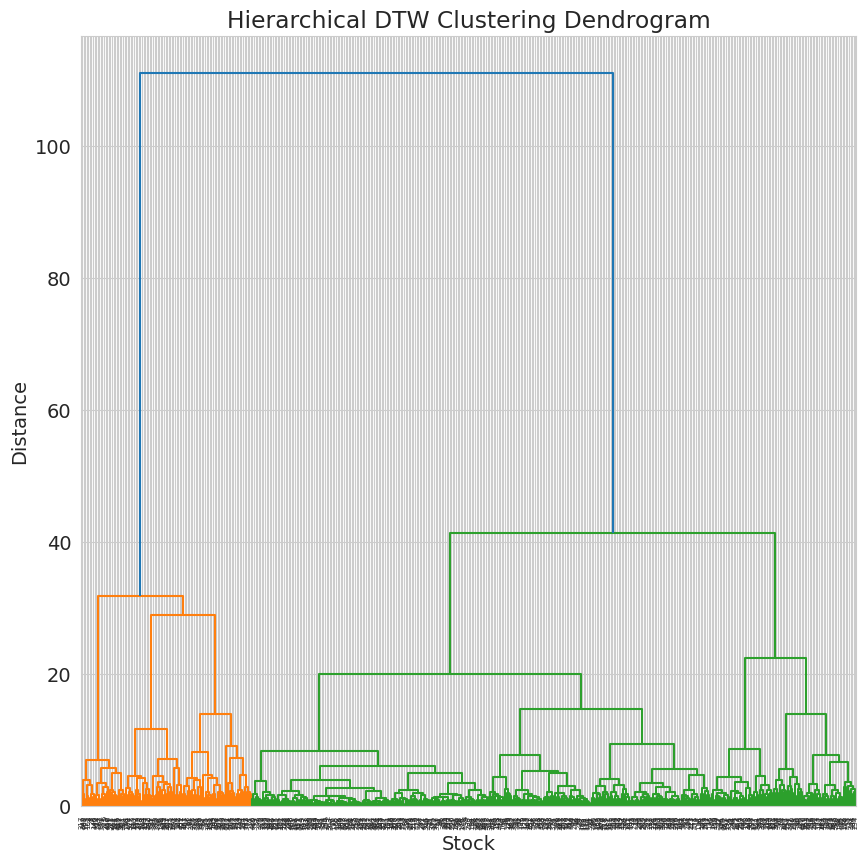
\includegraphics[width=11cm]{img/dendogram.png} 
\caption{Hierarchical dendrogram for Ward's minimum}
\label{fig:kernel_dendrogram}
\end{figure}

The exact identity of each stock is not discernible from the dendrogram due to the density of labels, but each vertical line corresponds to a stock or a cluster of stocks. It illustrates a couple of splits which are significant in distance, and the closer we get to the bottom of the diagram the less significant the difference between stocks is considered. 

Now we will look at the method we have chosen to proceed with for linkage (Ward).

\begin{figure}[H]
\centering
\label{fig:kernel_average_dendrogram}
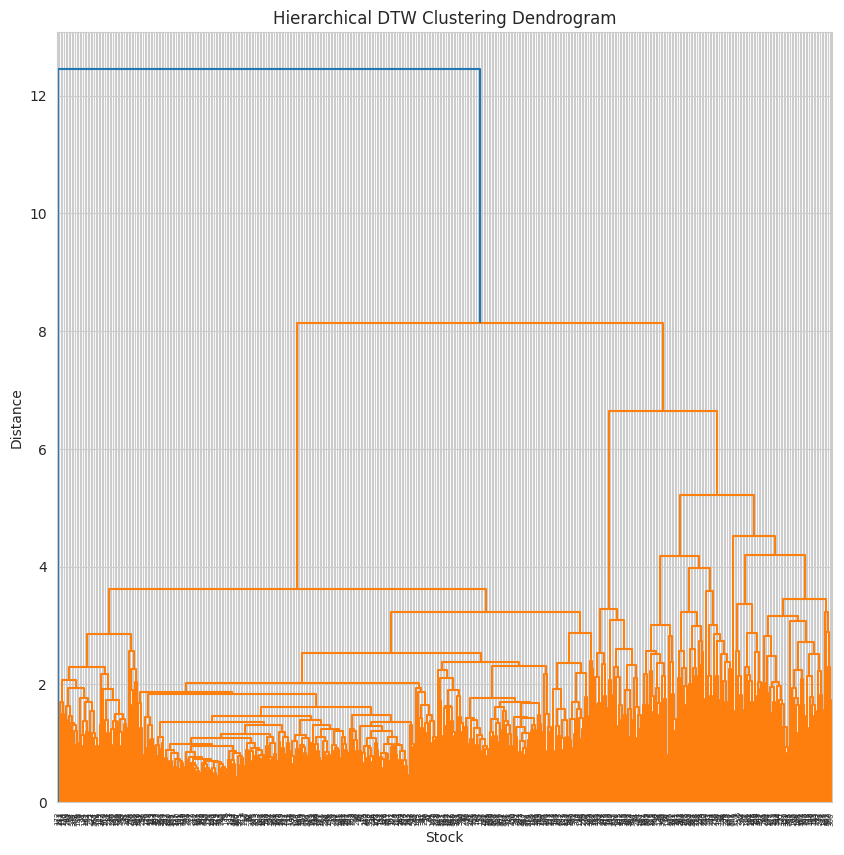
\includegraphics[width=11cm]{img/dendogram_average.png} 
\caption{Hierarchical dendrogram for Average}
\end{figure}

Using the averaging methodology we can see the later splits are much taller than in Ward (Fig. \ref{fig:kernel_dendrogram}), suggesting the potential to have identified more distinctive attributes. However, when we examine the distribution of stocks in clusters, it becomes evident that the average linkage technique produces a notably higher number of outliers. This observation holds true irrespective of the predetermined number of clusters, presenting a stark contrast to the results obtained using Ward's minimum variance method. The skewed distributions of stocks in clusters can be observed in the following:

\begin{figure}[H]
\centering
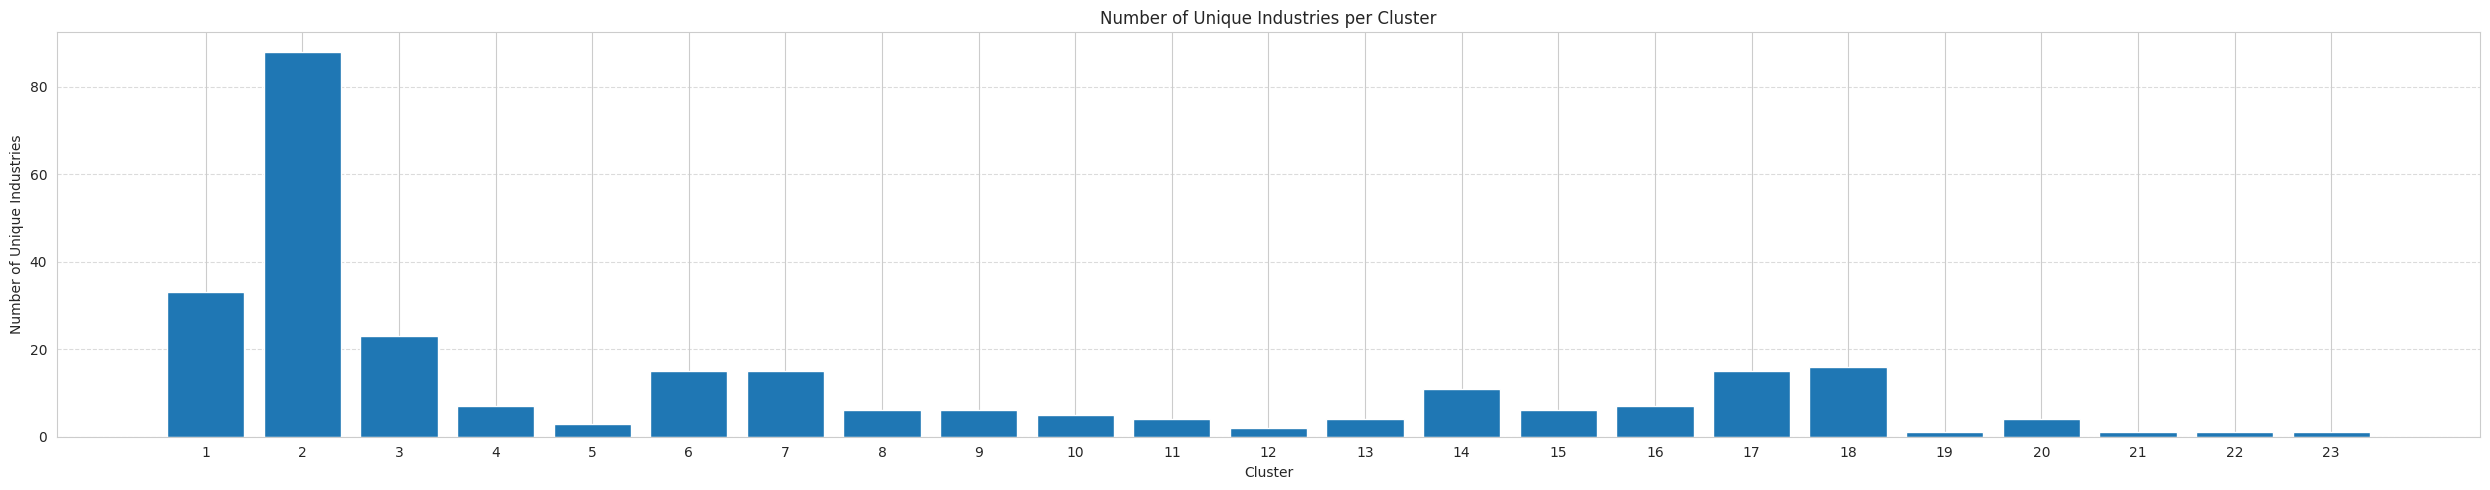
\includegraphics[width=12cm]{img/hierarchical_average.png} 
\caption{Stocks in clusters for hierarchical dendrogram using Average distance}
\label{fig:average_dendrogram}
\end{figure}

We conclude that we should use Ward's minimum and that it will be useful to split our data in 23 (square root of our data) clusters to reach a point of diminishing returns where the distance is no longer significant enough to warrant further sub-grouping. With our choice of 23 clusters, we try to identify the most recognisable patterns, reducing the distance sensibly in the context of DTW.

\subsubsection{Application in Stocks}

Running on our entire data-set of 491 stocks, we have configured a partitioning of the 23 clusters (square root of the 491 stocks) in a parallel computing environment. This took 60 minutes to compile the model and under 5 seconds to generate clusters. The extended compilation time is attributed to the necessity of computing a pairwise matrix capturing the Dynamic Time Warping (DTW) distances between every pair of stocks.

\begin{figure}[H]
\centering
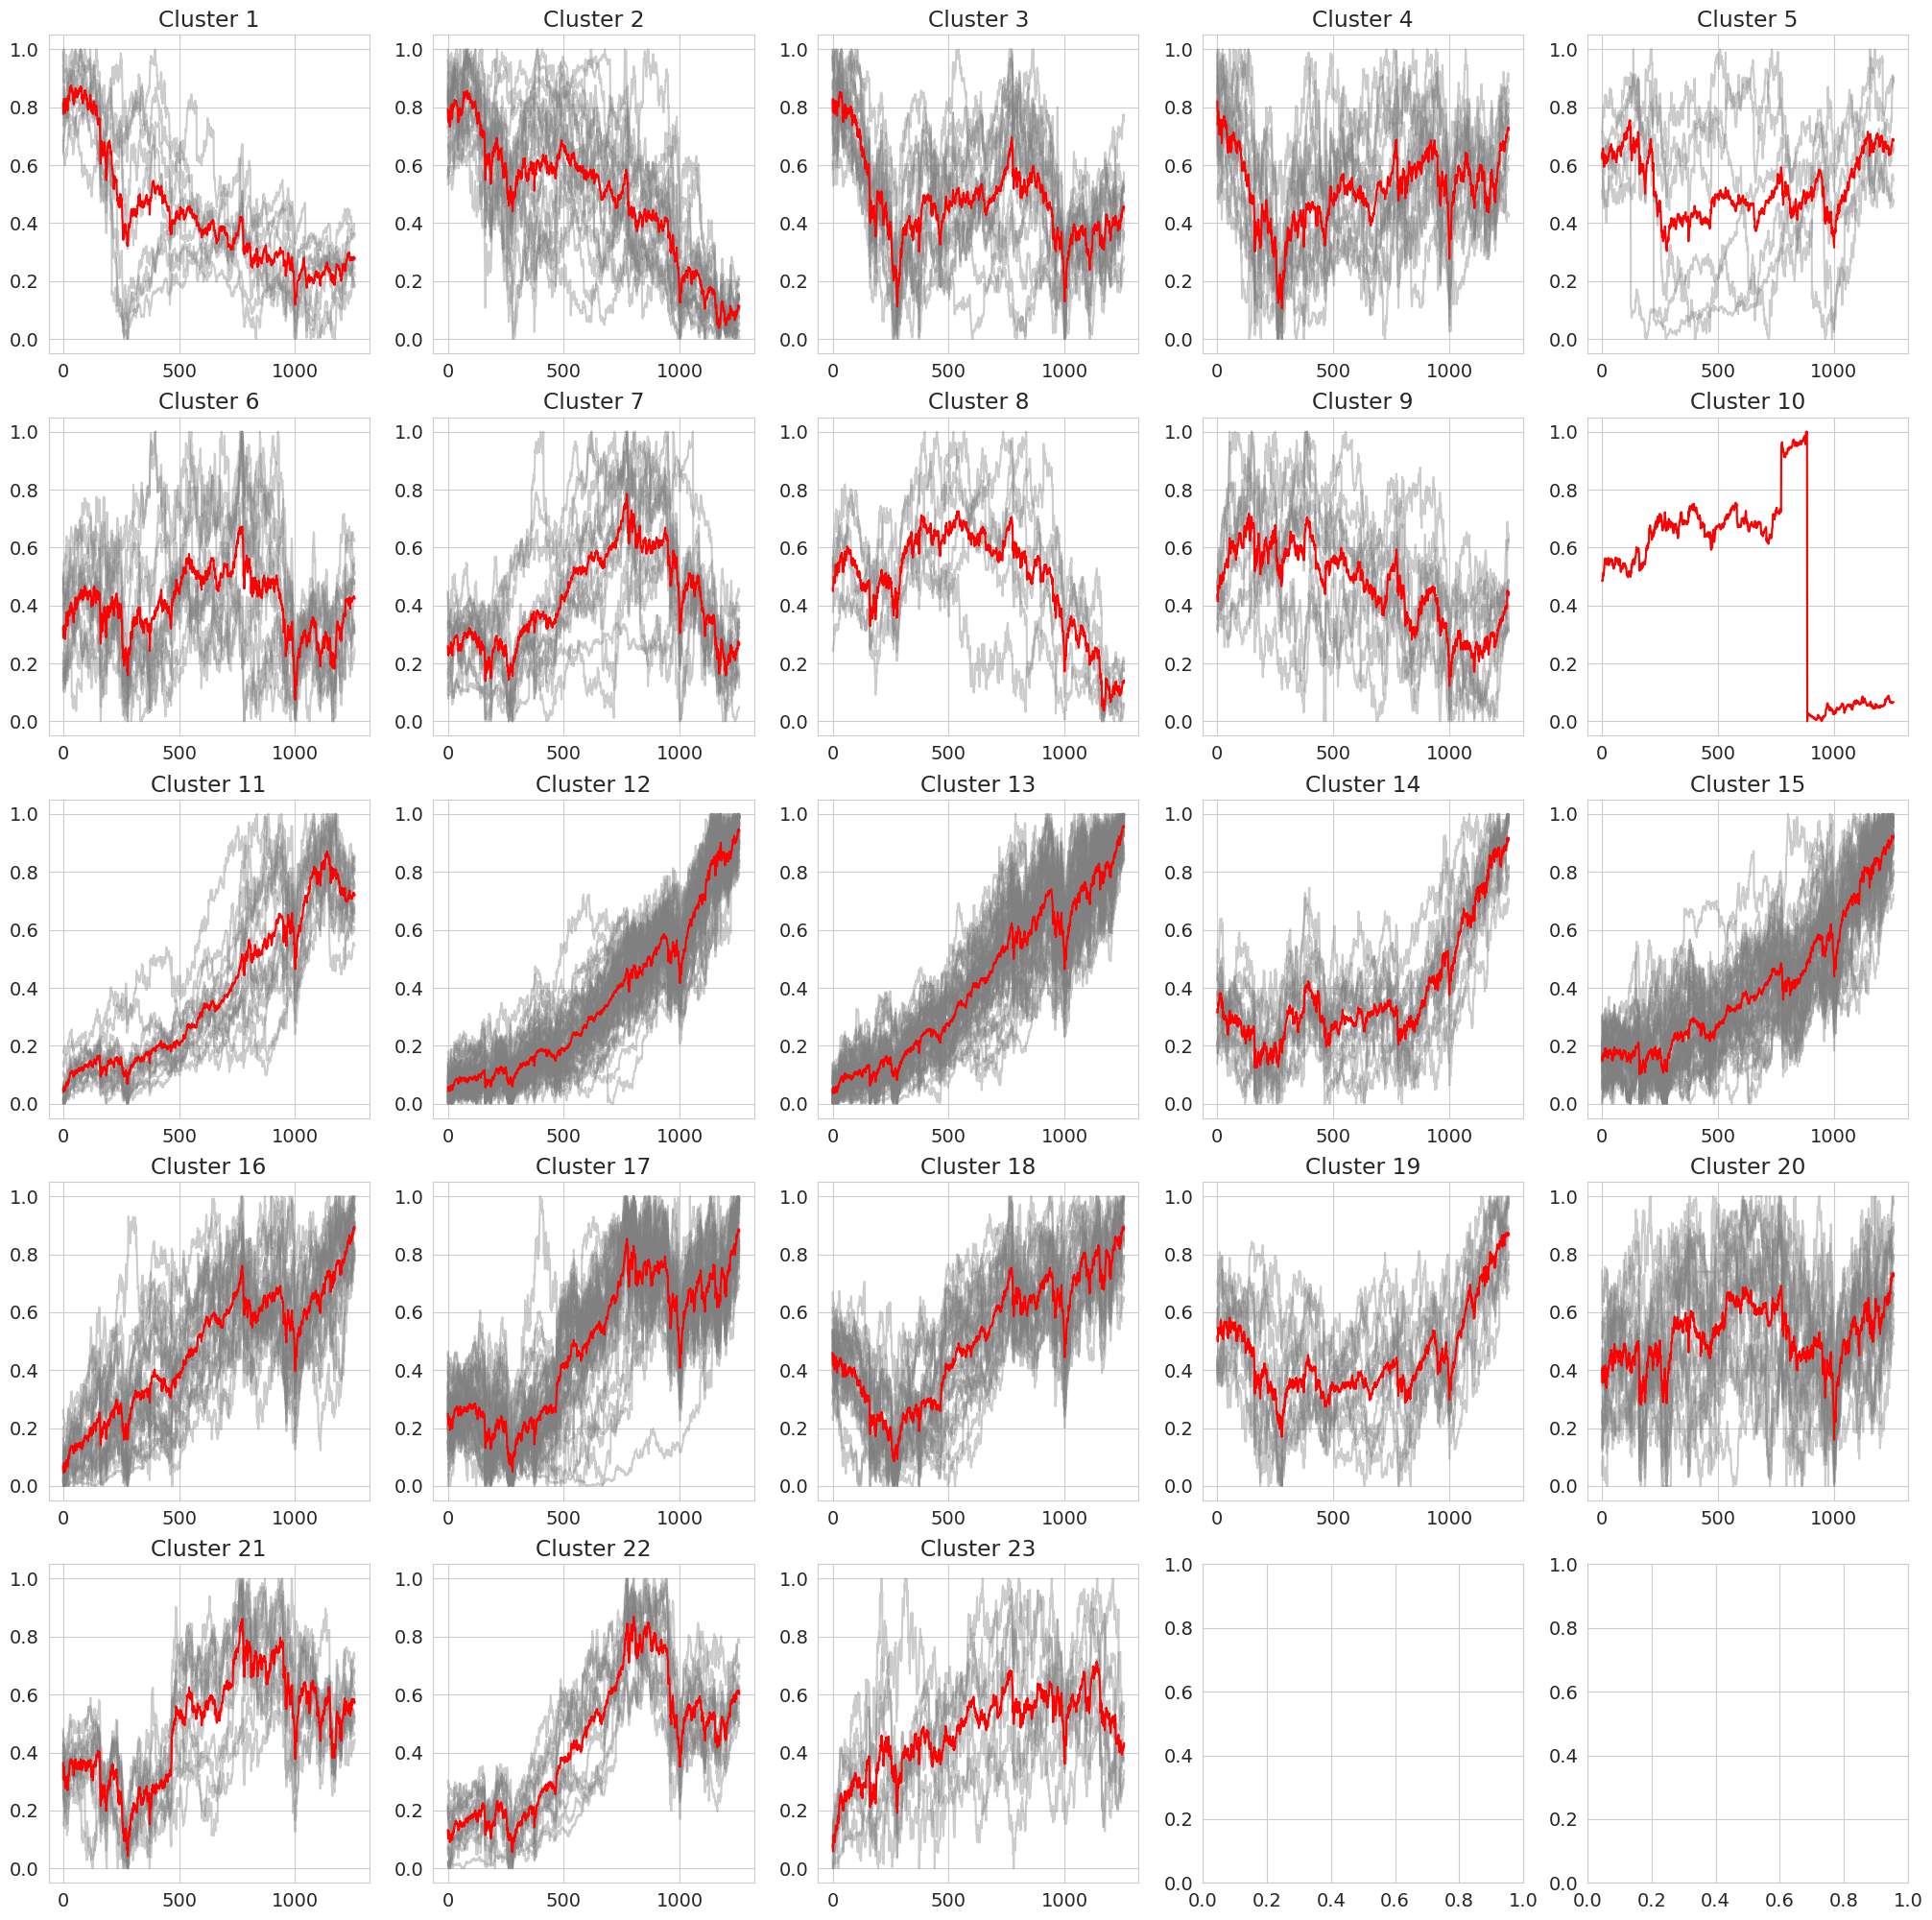
\includegraphics[width=12cm]{img/kernel-average.png} 
\caption{Averaged centroid for hierarchical clusters}
\label{fig:kernel-average}
\end{figure}

Compared to K-Means Euclidean (Fig. \ref{fig:kmeans_average}), we can see that each cluster is more noisy visually due to grouped stocks having similar behaviours at different points in time. In other words, lines within each cluster have similar shapes asynchronously. 

When contrasting this methodology with the traditional K-Means utilising Euclidean distance, one notable distinction is obvious in \textit{Cluster 10}, with a single stock encapsulated from one company: KDP. A separate financial analysis reveals that in 2018, KDP experienced a pronounced decline in its stock valuation, attributable to a merger and contextual economic conditions of the time. Such unique circumstances render KDP distinct from its peers, leading to its classification as an anomaly and an outlier in our data:

\begin{figure}[H]
\centering
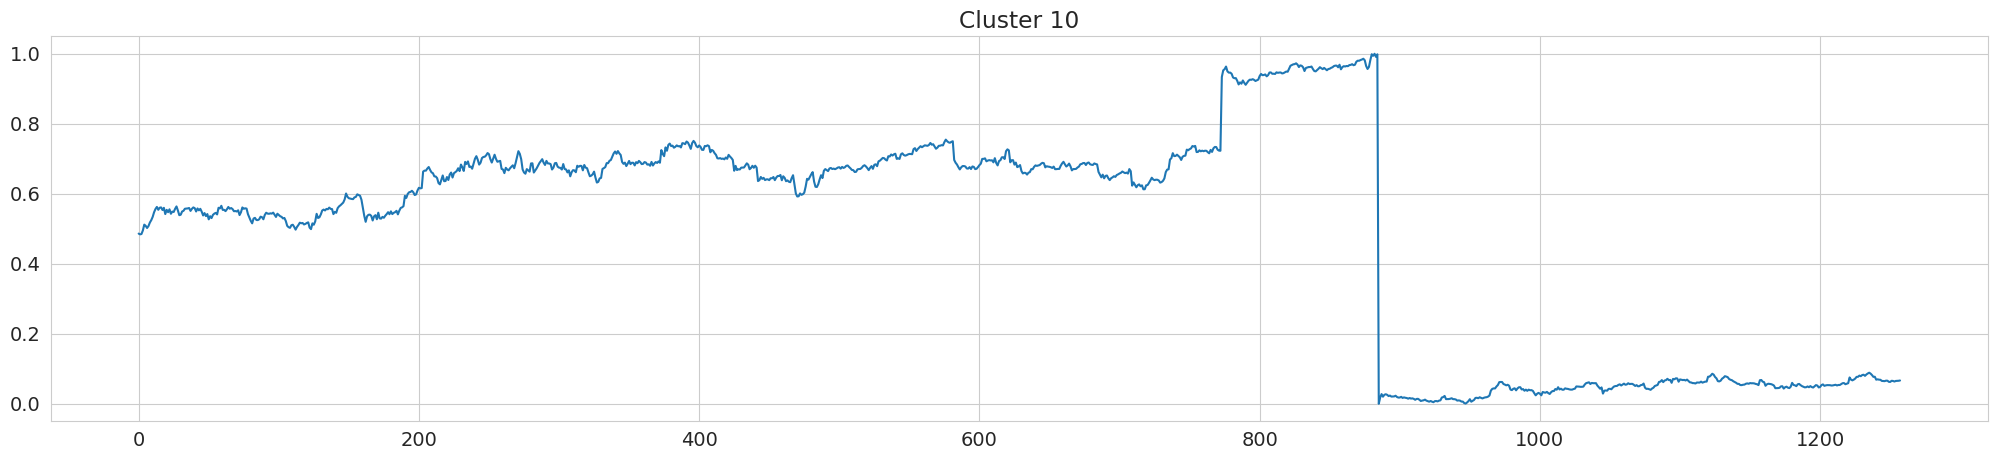
\includegraphics[width=12cm]{img/kernel-cluster10.png} 
\caption{Cluster 10 as an outlier - KDP}
\label{fig:kernel-cluster10}
\end{figure}

If we cherry-pick another cluster, say \textit{Cluster 5}, to deep-dive into the detected patterns, we can see similar behaviours at different points in time which mirrors the previously presented example in Fig. \ref{fig:mtch-bax} that contained the MTCH and BAX companies. They are also included in our selected \textit{Cluster 5}, alongside AIG, AAP, XRAY, and CF.

\begin{figure}[H]
\centering
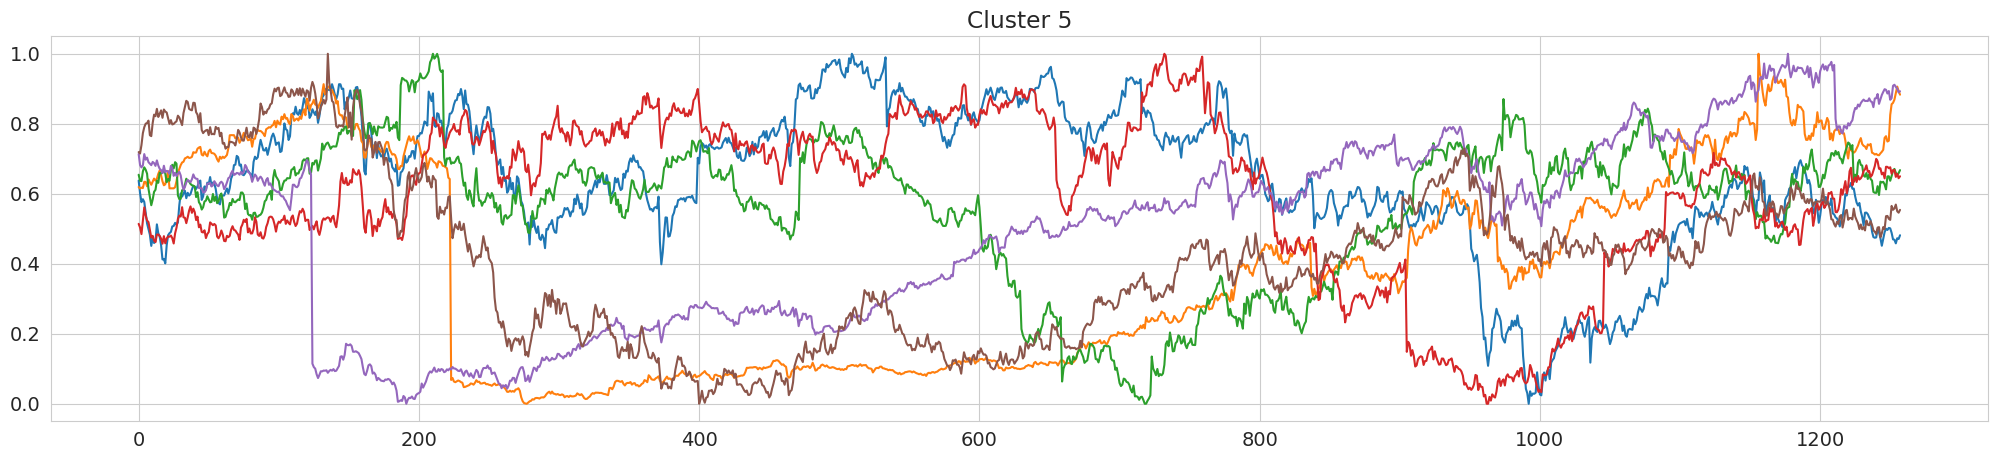
\includegraphics[width=12cm]{img/kernel-cluster5.png} 
\caption{Cluster 5 spotlight - MTCH, BAX, AIG, AAP, XRAY, and CF}
\label{fig:kernel-cluster5}
\end{figure}

\begin{figure}[H] 
\centering
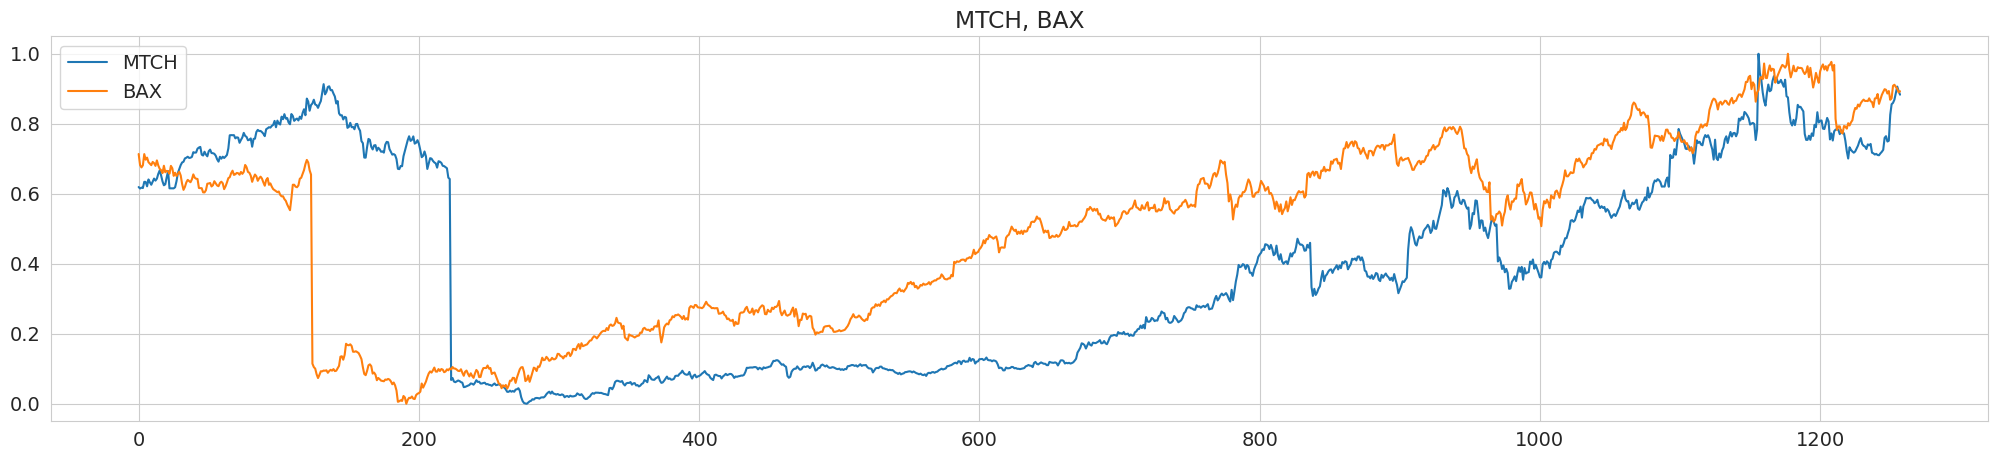
\includegraphics[width=12cm]{img/mtch-bax.png} 
\caption{MTCH and BAX stocks in hierarchical DTW Cluster 5}
\end{figure}

K-Means Euclidean did not capture this correlation in the previous section, putting the two stocks in \textit{Cluster 11} and \textit{Cluster 20} respectively (Fig. \ref{fig:kmeans_average}). Thus, we can see the benefits of leveraging DTW distances.

We have recorded the following standard metrics:
\begin{itemize}
    \item \textit{Silhouette score:} 0.116
    \item \textit{Calinski-Harabasz index:} 28.772
    \item \textit{Davies-Bouldin index:} 2.936
\end{itemize}

A comparison of these scores for all algorithms can be found in the \textit{\hyperref[sec:compare]{Scoring and Comparison}} section.


\begin{figure}[H]
\centering
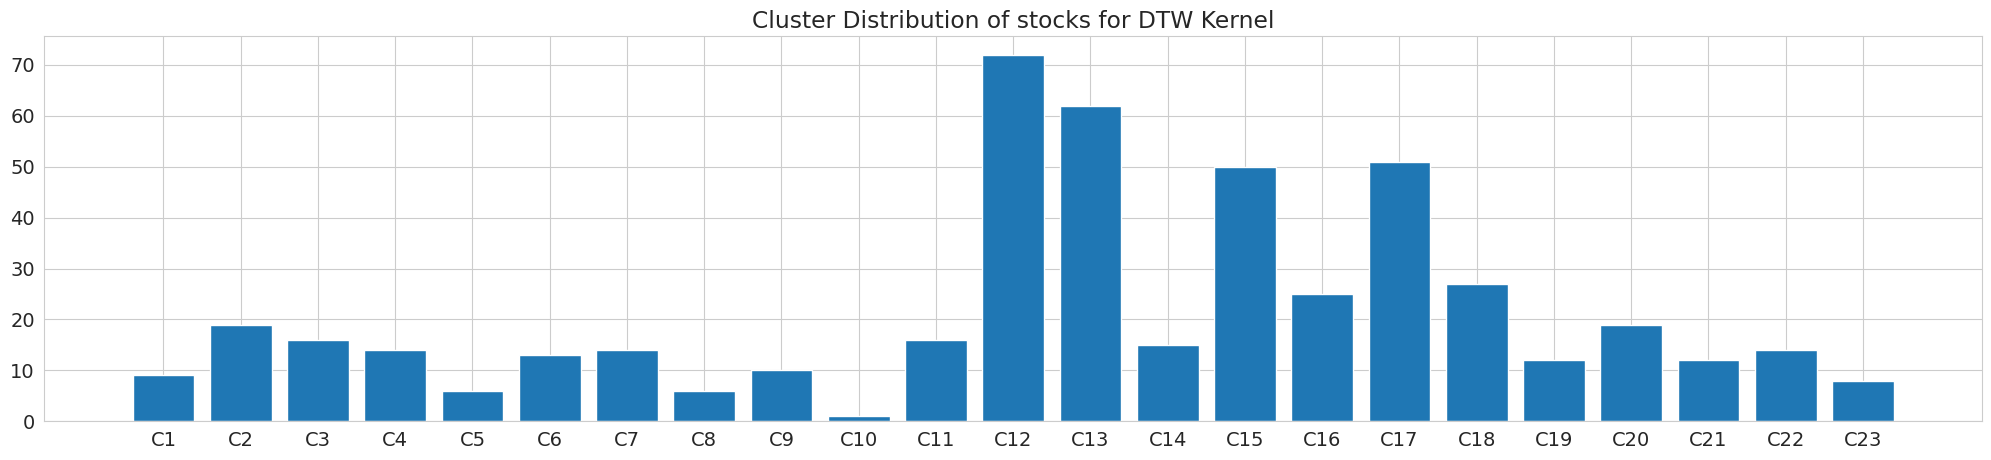
\includegraphics[width=12cm]{img/kernel-dtw-stock-distrib.png} 
\caption{Distribution of stocks within their hierarchical clusters}
\label{fig:kmeans_dtw_dist}
\end{figure}

In terms of distribution per cluster, 7 of them contain a disproportionate amount of the stocks. This further confirms the noisiness we have inferred from the average line (Fig. \ref{fig:dtw_kmeans_average}). Simply having a high number of stocks in a cluster does not signify if they are a good match to one another and form a pattern.

\begin{figure}[H]
\centering
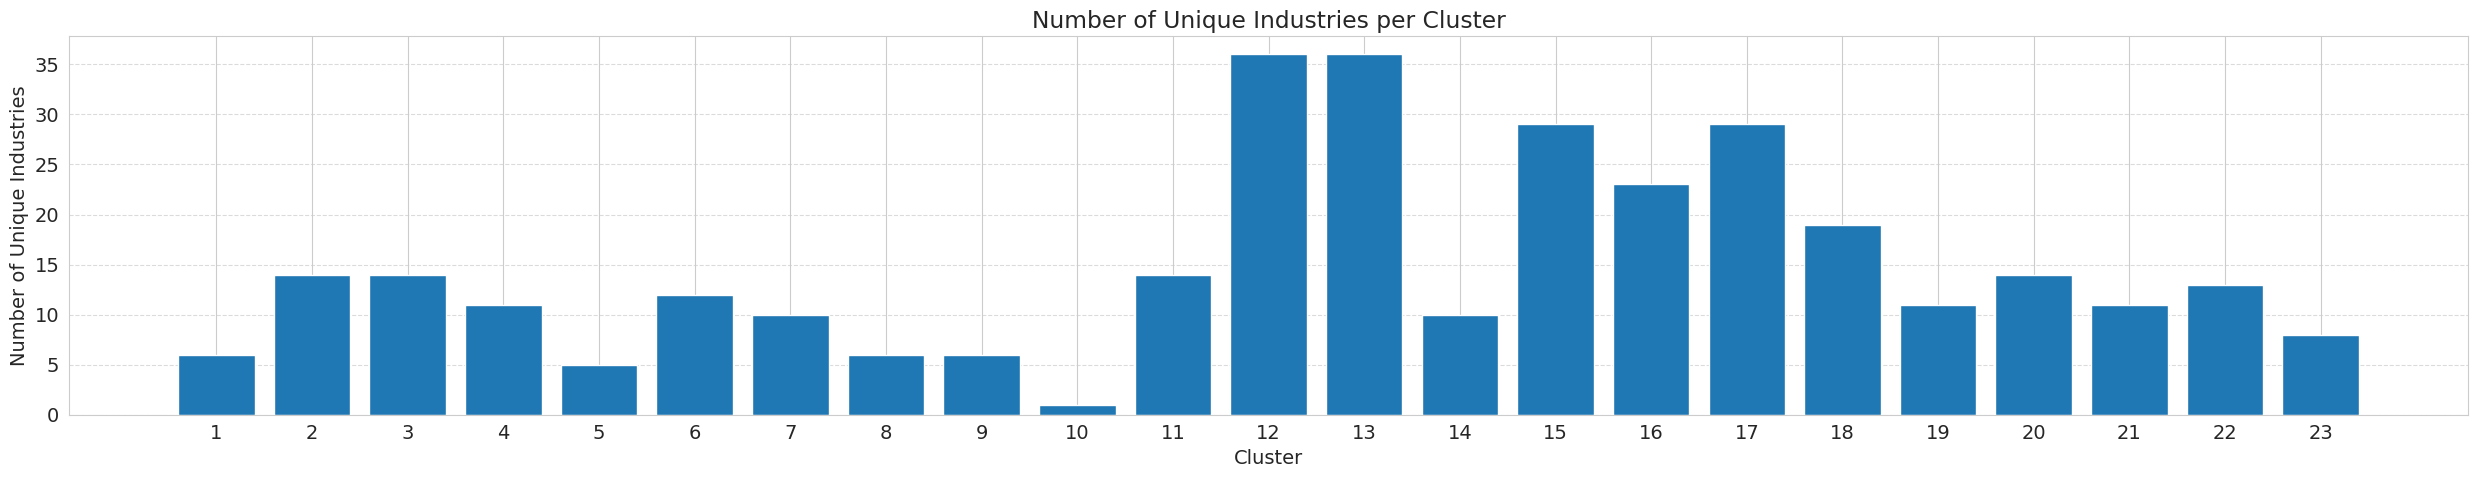
\includegraphics[width=12cm]{img/kernel-industries.png} 
\caption{Distribution of industries in their hierarchical clusters}
\label{fig:kernel_industries}
\end{figure}

Just as observed in K-Means Euclidean (Fig. \ref{fig:kmeans_industries}) we maintain a direct correlation between the number of stocks and the number of industries. 

\subsection{MiniSom}
\subsubsection{Overview}

MiniSom, short for Mini Self-Organising Map (SOM), is an unsupervised machine learning algorithm used for clustering and visualising high-dimensional data. It is a type of artificial neural network that is capable of finding patterns in the data and creating a low-dimensional representation of the data in the form of a map. 

 MiniSom is capable of capturing the shape similarities between time-series data points, even if they are temporally misaligned, making it a perfect candidate for our use case of analysing asynchronous stock prices that might behave similarly. 
 
\subsubsection{Algorithm}

In traditional MiniSom, the winner neuron \( b(x) \) is usually identified based on the Euclidean distance between it and other nodes as follows:

\begin{equation*}
b(x) = \arg \min_{i} || x - w_i ||
\end{equation*}


The weight update rule for the winner stock and its neighbours is as follows:

\begin{equation*}
w_{i}(t+1) = w_{i}(t) + \alpha(t) \cdot h_{ib}(t) \cdot (x - w_{i}(t))
\end{equation*}

Where \( \alpha(t) \) is a time-decreasing learning rate, and \( h_{ib}(t) \) is a neighbourhood function centred around the winner stock \( b \).


MiniSom is a lightweight and Numpy-based implementation of Self-Organising Maps (SOMs), also known as Kohonen maps. 


\subsubsection{Application in Stocks}

To be consistent with the approach used for the other algorithms, we have selected 23 as the square root of the total stocks in our data-set. Running on our entire data-set of 491 stocks, we have done an initial configuration of the 23 clusters, which took 20 seconds to compile the model and predict.  

If we plot our three standard scores against the number of clusters we could configure, we can observe the following:

\begin{figure}[H]
\centering
\includegraphics[width=8cm]{img/MiniSom-index-comparison.png} 
\caption{MiniSom scores while tweaking the size of matrix}
\end{figure}

\begin{itemize}
    \item Silhouette score is minimised, as expected.
    \item Calinski-Harabasz is also minimised, behaving similarly to the same score in the K-Means Euclidean algorithm.
    \item Davies-Bouldin, though also trending towards 0, seems to be on the larger end, numbers-wise.
\end{itemize}

Through this, we can see how the general metrics leveraged are not fairly representing the clusters due to their asynchronous nature and diverse behaviour, which causes them to have a higher score when many of them are together in fewer clusters.

By conducting a visual inspection of our clusters using a  DTW Barycenter Averaging centroid approach, we could subjectively observe trends within each cluster, regardless of the scores obtained:

\begin{figure}[H]
\centering
\includegraphics[width=12cm]{img/MiniSom-dba.png} 
\caption{MiniSom Barycenter Averaging (DBA)}
\label{fig:minisom_dba}
\end{figure}

Compared to the DTW Flat Clusters algorithm and K-Means, the visual output of DBA-based analysis is less noisy, where trend lines with similar shapes fit more closely together. This can be seen clearly in \textit{Cluster 18}:

\begin{figure}[H]
\centering
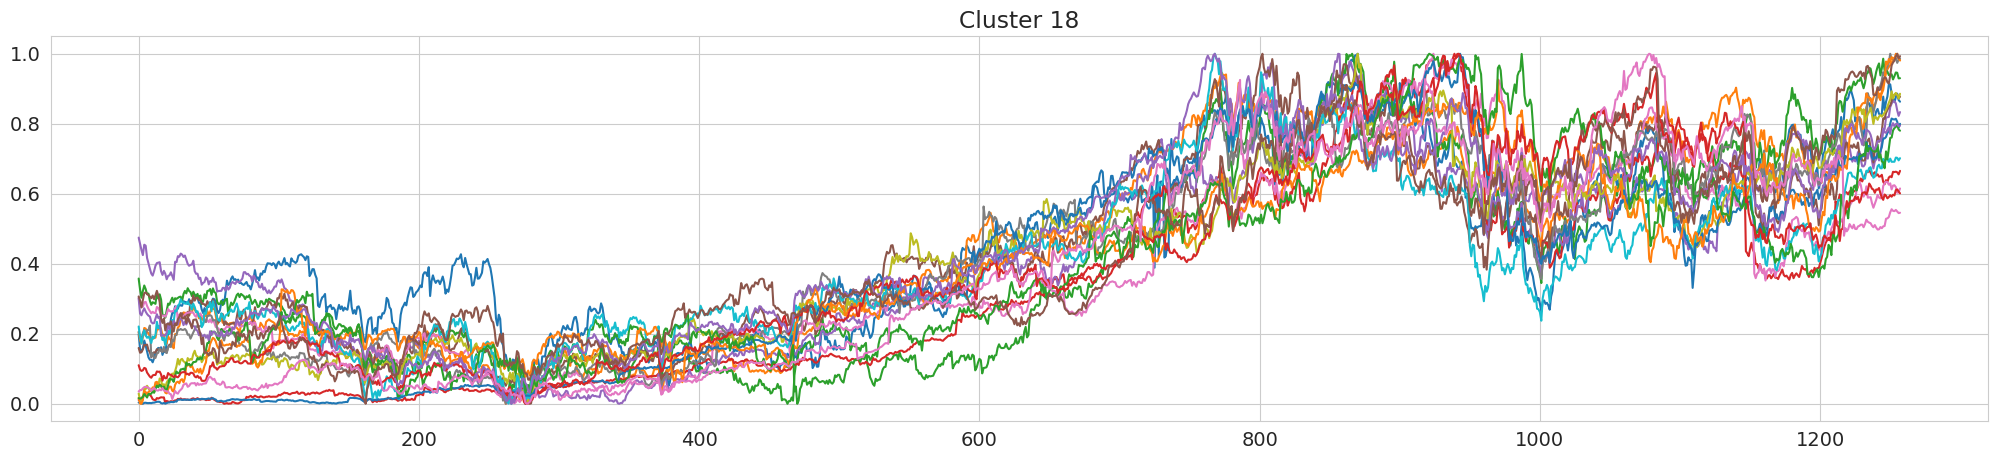
\includegraphics[width=12cm]{img/minisom-cluster18.png} 
\caption{MiniSom - Cluster 18 stocks}

\end{figure}

Additionally, the outlier identified by the flat clusters algorithm (Fig. \ref{fig:kernel-average}) is no longer an outlier with MiniSom, having been grouped in \textit{Cluster 5}.


MiniSom clustering scored as follows in our tracked metrics:
\begin{itemize}
    \item \textit{Silhouette score:} 0.11
    \item \textit{Calinski-Harabasz index:} 67.2
    \item \textit{Davies-Bouldin index:} 1.85
\end{itemize}


A comparison of these scores for all algorithms can be found in the \textit{\hyperref[sec:compare]{Scoring and Comparison}} section.

\begin{figure}[H]
\centering
\includegraphics[width=12cm]{img/MiniSom-distrib.png} 
\caption{Distribution of stocks within their MiniSom clusters}
\label{fig:minisom_distribution}
\end{figure}

MiniSom has achieved the smoothest distribution of stocks in clusters, compared to our other algorithms: Euclidean DTW (Fig. \ref{fig:euclidean_distrib}), DTW K-Means (Fig. \ref{fig:dtw_kmeans_distribution}), DTW K-Means PCA (Fig. \ref{fig:dtw_kmeans_pca_distribution}).


\begin{figure}[H]
\centering
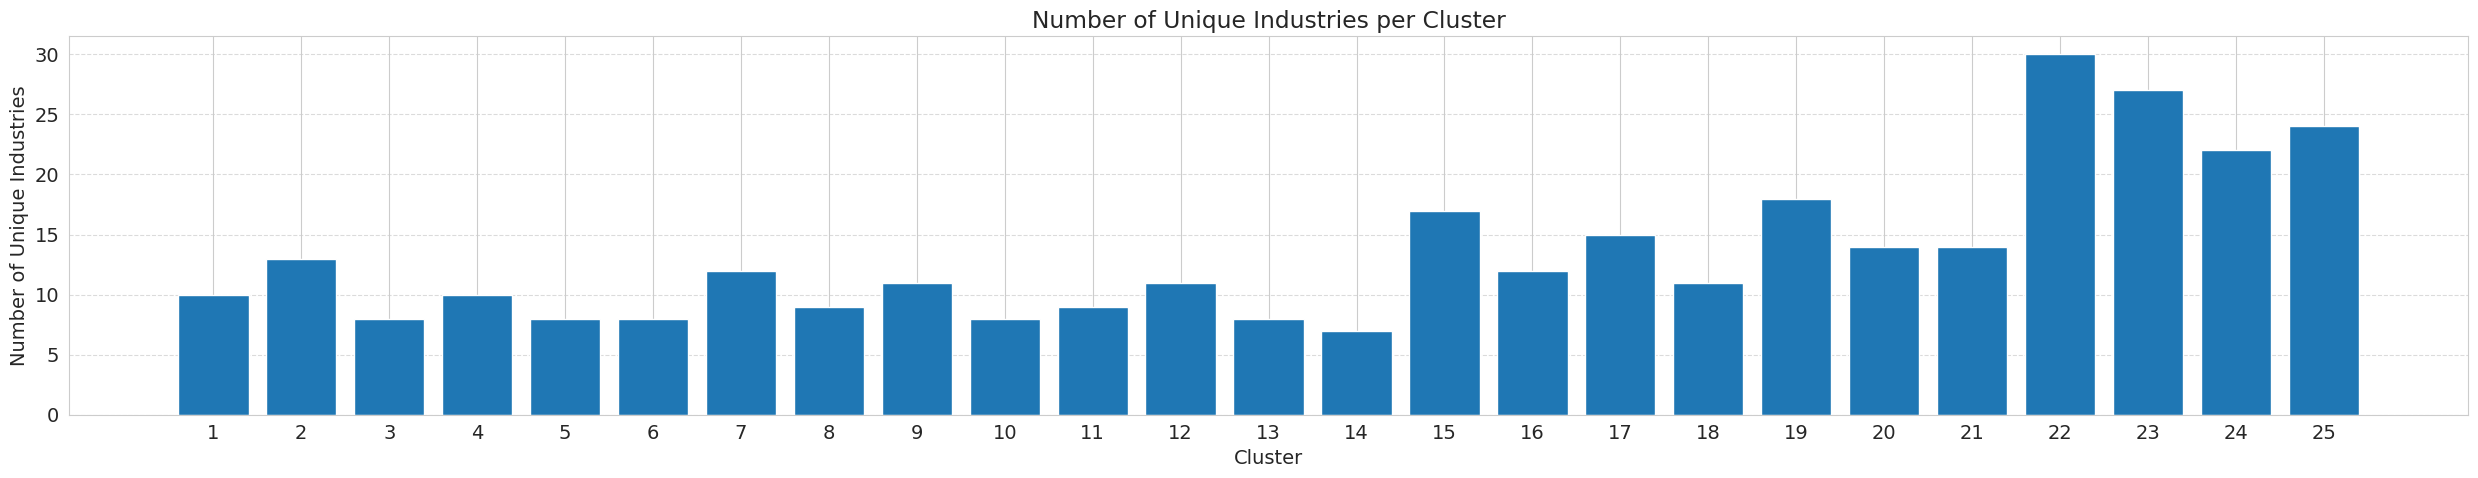
\includegraphics[width=12cm]{img/minisom-industries.png} 
\caption{Distribution of industries in their MiniSom clusters}
\label{fig:minisom_industries}
\end{figure}

Similarly to the other algorithms, we maintain direct proportionality between the number of stocks and the number of industries. This is most beneficial in this scenario, as the stocks are more uniformly distributed in their clusters (Fig. \ref{fig:minisom_distribution}), without biasing the clusters into specific industries. 

\subsection{K-Means DTW}
\subsubsection{Overview}

In this section, we explore the K-Means algorithm adapted to make use of Dynamic Time Warping distance for clustering rather than Euclidean-based matching. 

\subsubsection{Algorithm}

In K-Means with DTW, the objective is to minimise the intra-cluster sum of DTW distances between stock time-series:


\begin{equation}
\underset{\mathbf{c}_1, \mathbf{c}_2, ..., \mathbf{c}_k}{\text{minimise}} \sum_{i=1}^{k} \sum_{S \in C_i} \text{DTW}(S, \mathbf{c}_i)^2
\end{equation}

Where:
\begin{itemize}
    \item \( \mathbf{c}_i \) is the centroid of cluster \( C_i \).
    \item \( \text{DTW}(S, \mathbf{c}_i) \) is the DTW distance between a time-series for stock \( S \) and the centroid \( \mathbf{c}_i \).
    \item The inner sum is over all time-series \( T \) that belong to cluster \( C_i \).
    \item The outer sum is over all clusters.
\end{itemize}

Groups of similar shapes in time-series are collected in clusters, which is possible thanks to Dynamic Time Warping's capability to handle time shifts. Then, the barycenters, also known as cluster centres, are calculated based on DTW, which enables the retrieval of a meaningful average shape irrespective of the temporal shifts within the cluster. 


We have leveraged K-Means from the \textit{tslearn} library \cite{tslearnclustering} to test this methodology out. The K-Means algorithm in \textit{tslearn} minimises the following objective function:

$$\sum_{j=1}^k \sum_{X_i \in C_j} \sum_{t=1}^m (X_i(t) - \mu_j(t))^2$$

where $C_j$ is the set of time-series in cluster $j$, and $\mu_j$ is the centroid of cluster $j$:

$$\mu_j(t) = \frac{1}{|C_j|} \sum_{X_i \in C_j} X_i(t)$$

The K-Means algorithm incrementally assigns time-series to clusters and updates the centroids until convergence. At each iteration, the algorithm first assigns each time-series to the nearest centroid based on the distance between the time-series and the centroid:

$$d(X_i, \mu_j) = \sqrt{\sum_{t=1}^m (X_i(t) - \mu_j(t))^2}$$

Then, the algorithm updates the centroid locations based on the mean of the assigned time-series:

$$\mu_j(t) \leftarrow \frac{1}{|C_j|} \sum_{X_i \in C_j} X_i(t)$$

This process continues until the algorithm converges, meaning that there are no further changes in cluster assignments or centroid locations.

K-Means clustering is a powerful technique for clustering time-series data based on their similarities and differences. By minimising the intra-cluster sum of squares, K-Means can identify meaningful clusters of time-series that can help to reveal underlying patterns and relationships in the data.

\subsubsection{Application in Stocks}

Running on our entire data-set of 491 stocks, we have done an initial configuration of the 23 clusters, which took 20 minutes to run in our parallel computing environment. 

Running predictions using the resulting model to generate the clusters took 30 seconds.

\begin{figure}[H]
\centering
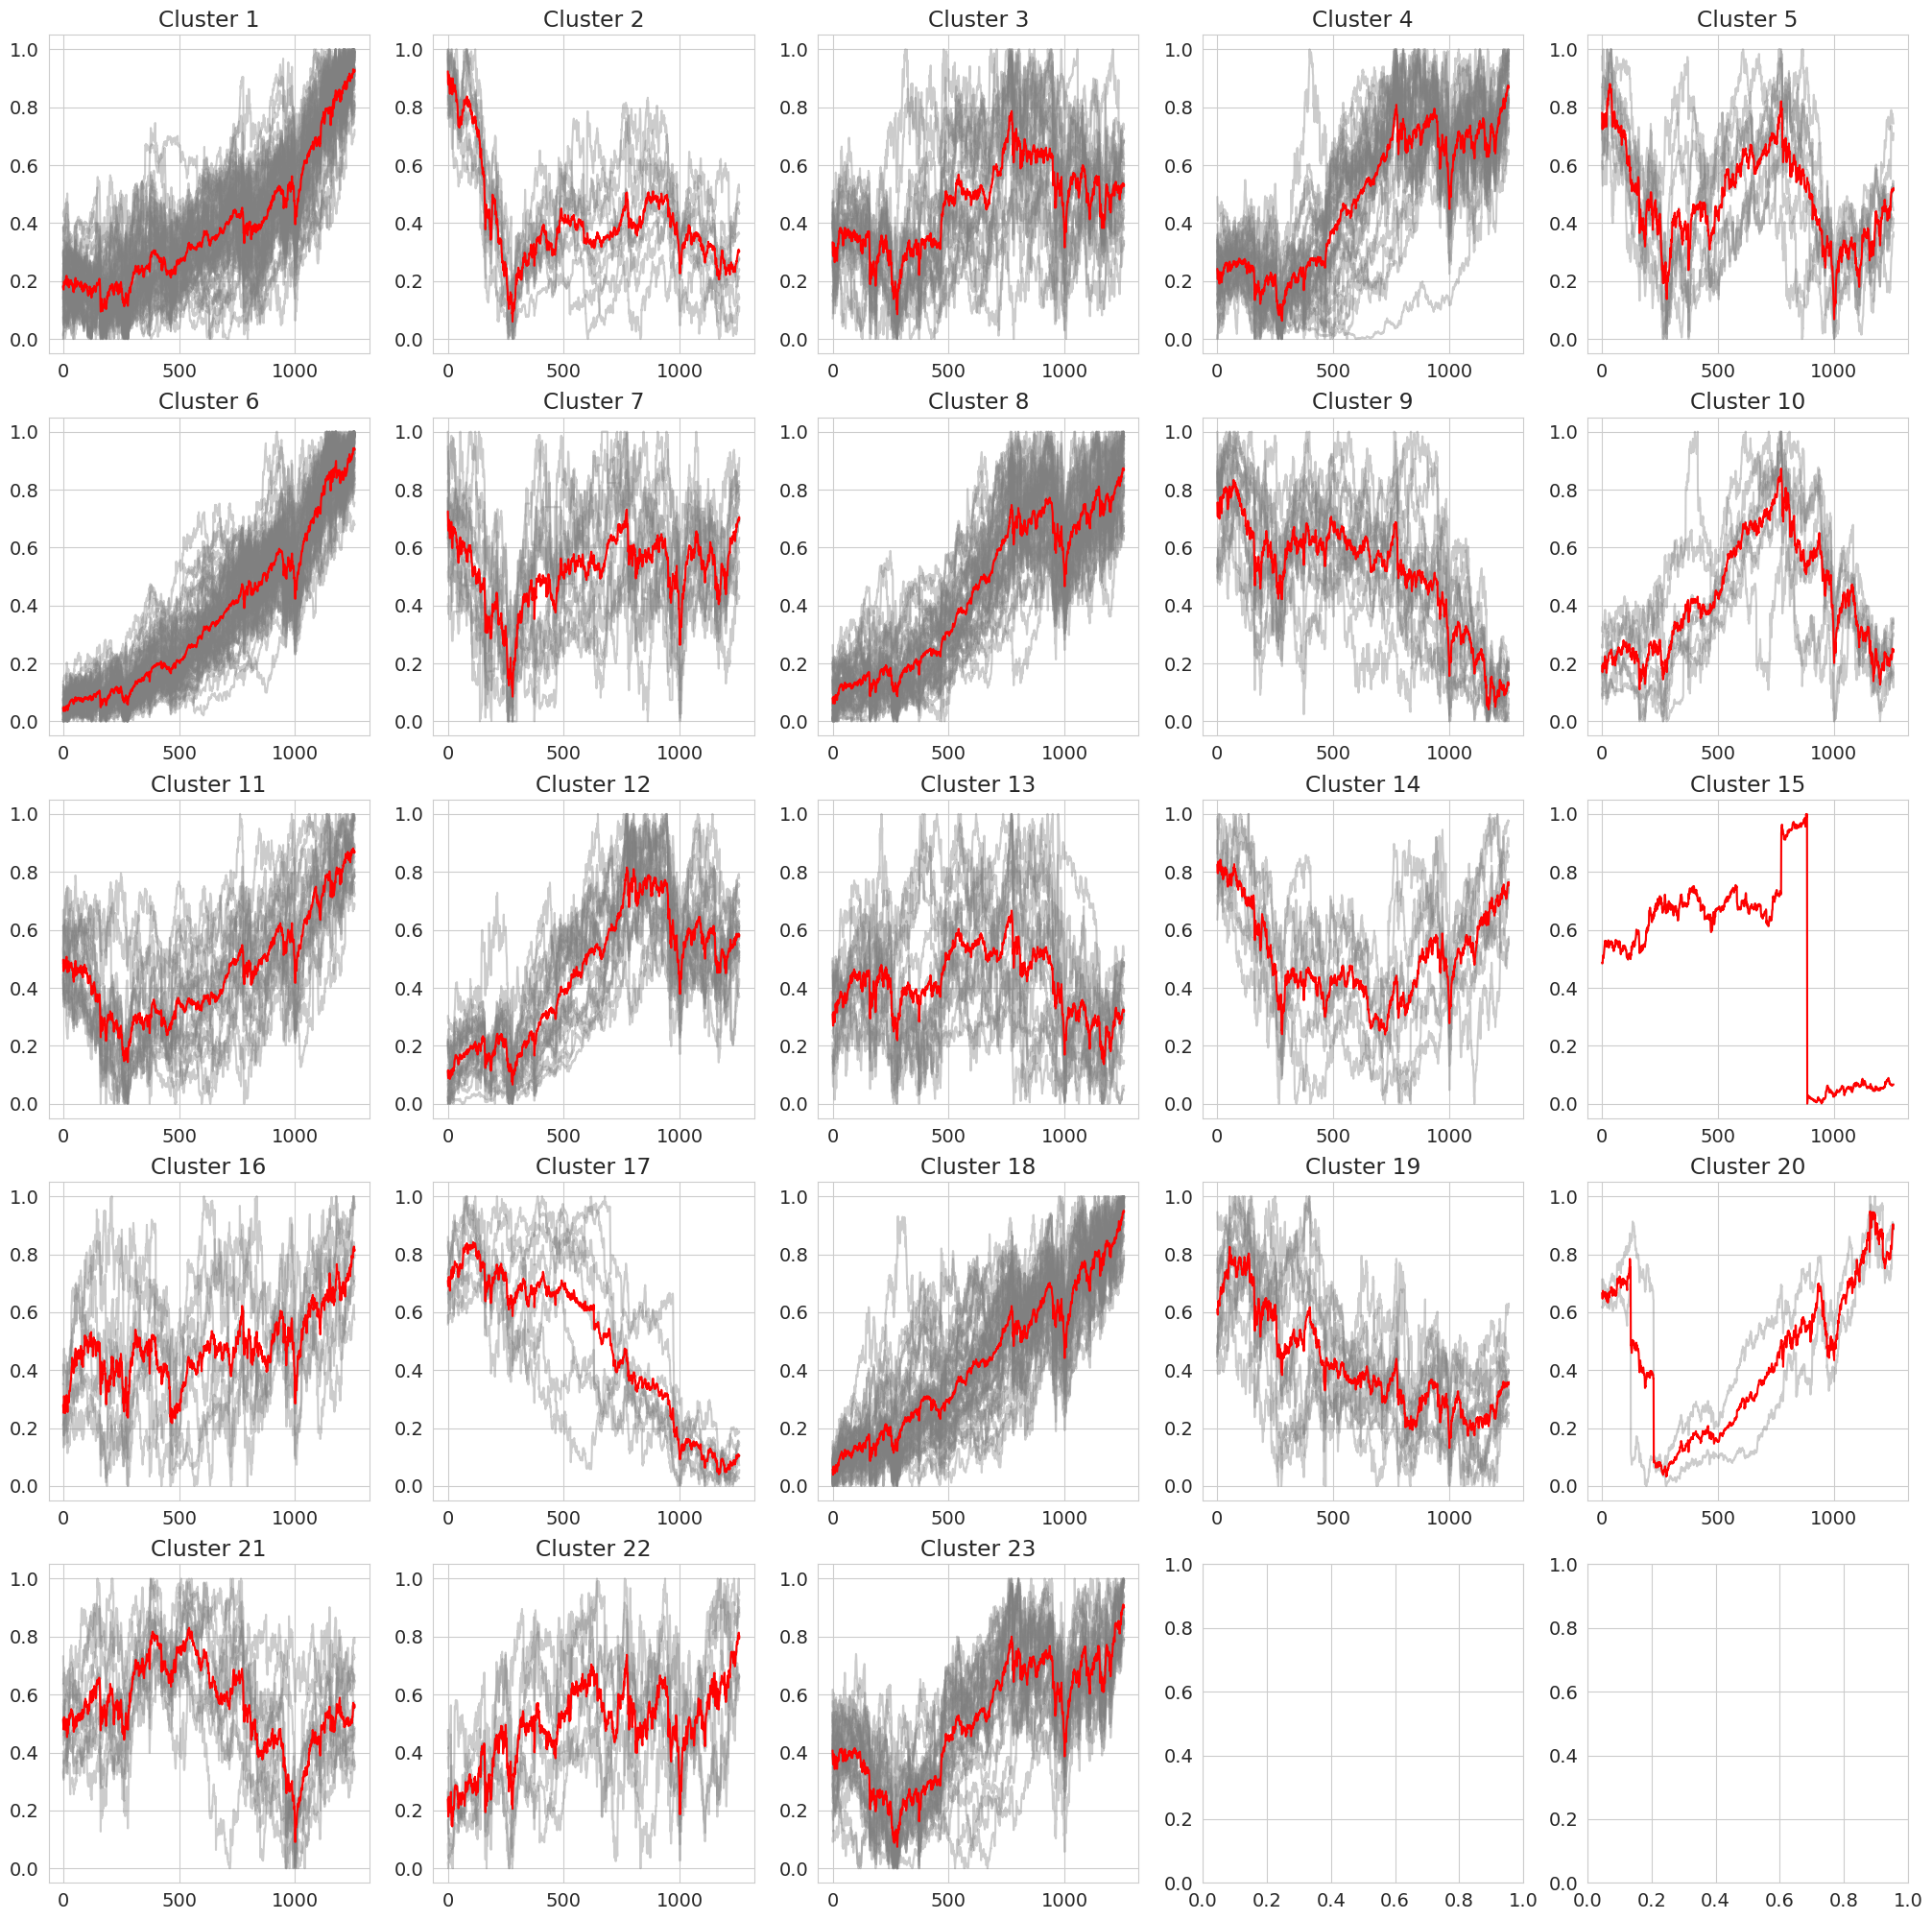
\includegraphics[width=12cm]{img/kmeands-ts-stocks.png} 
\caption{K-Means DTW clusters overlaid with averaged centroid line}
\label{fig:dtw_kmeans_average}

\end{figure}

\begin{figure}[H]
\centering
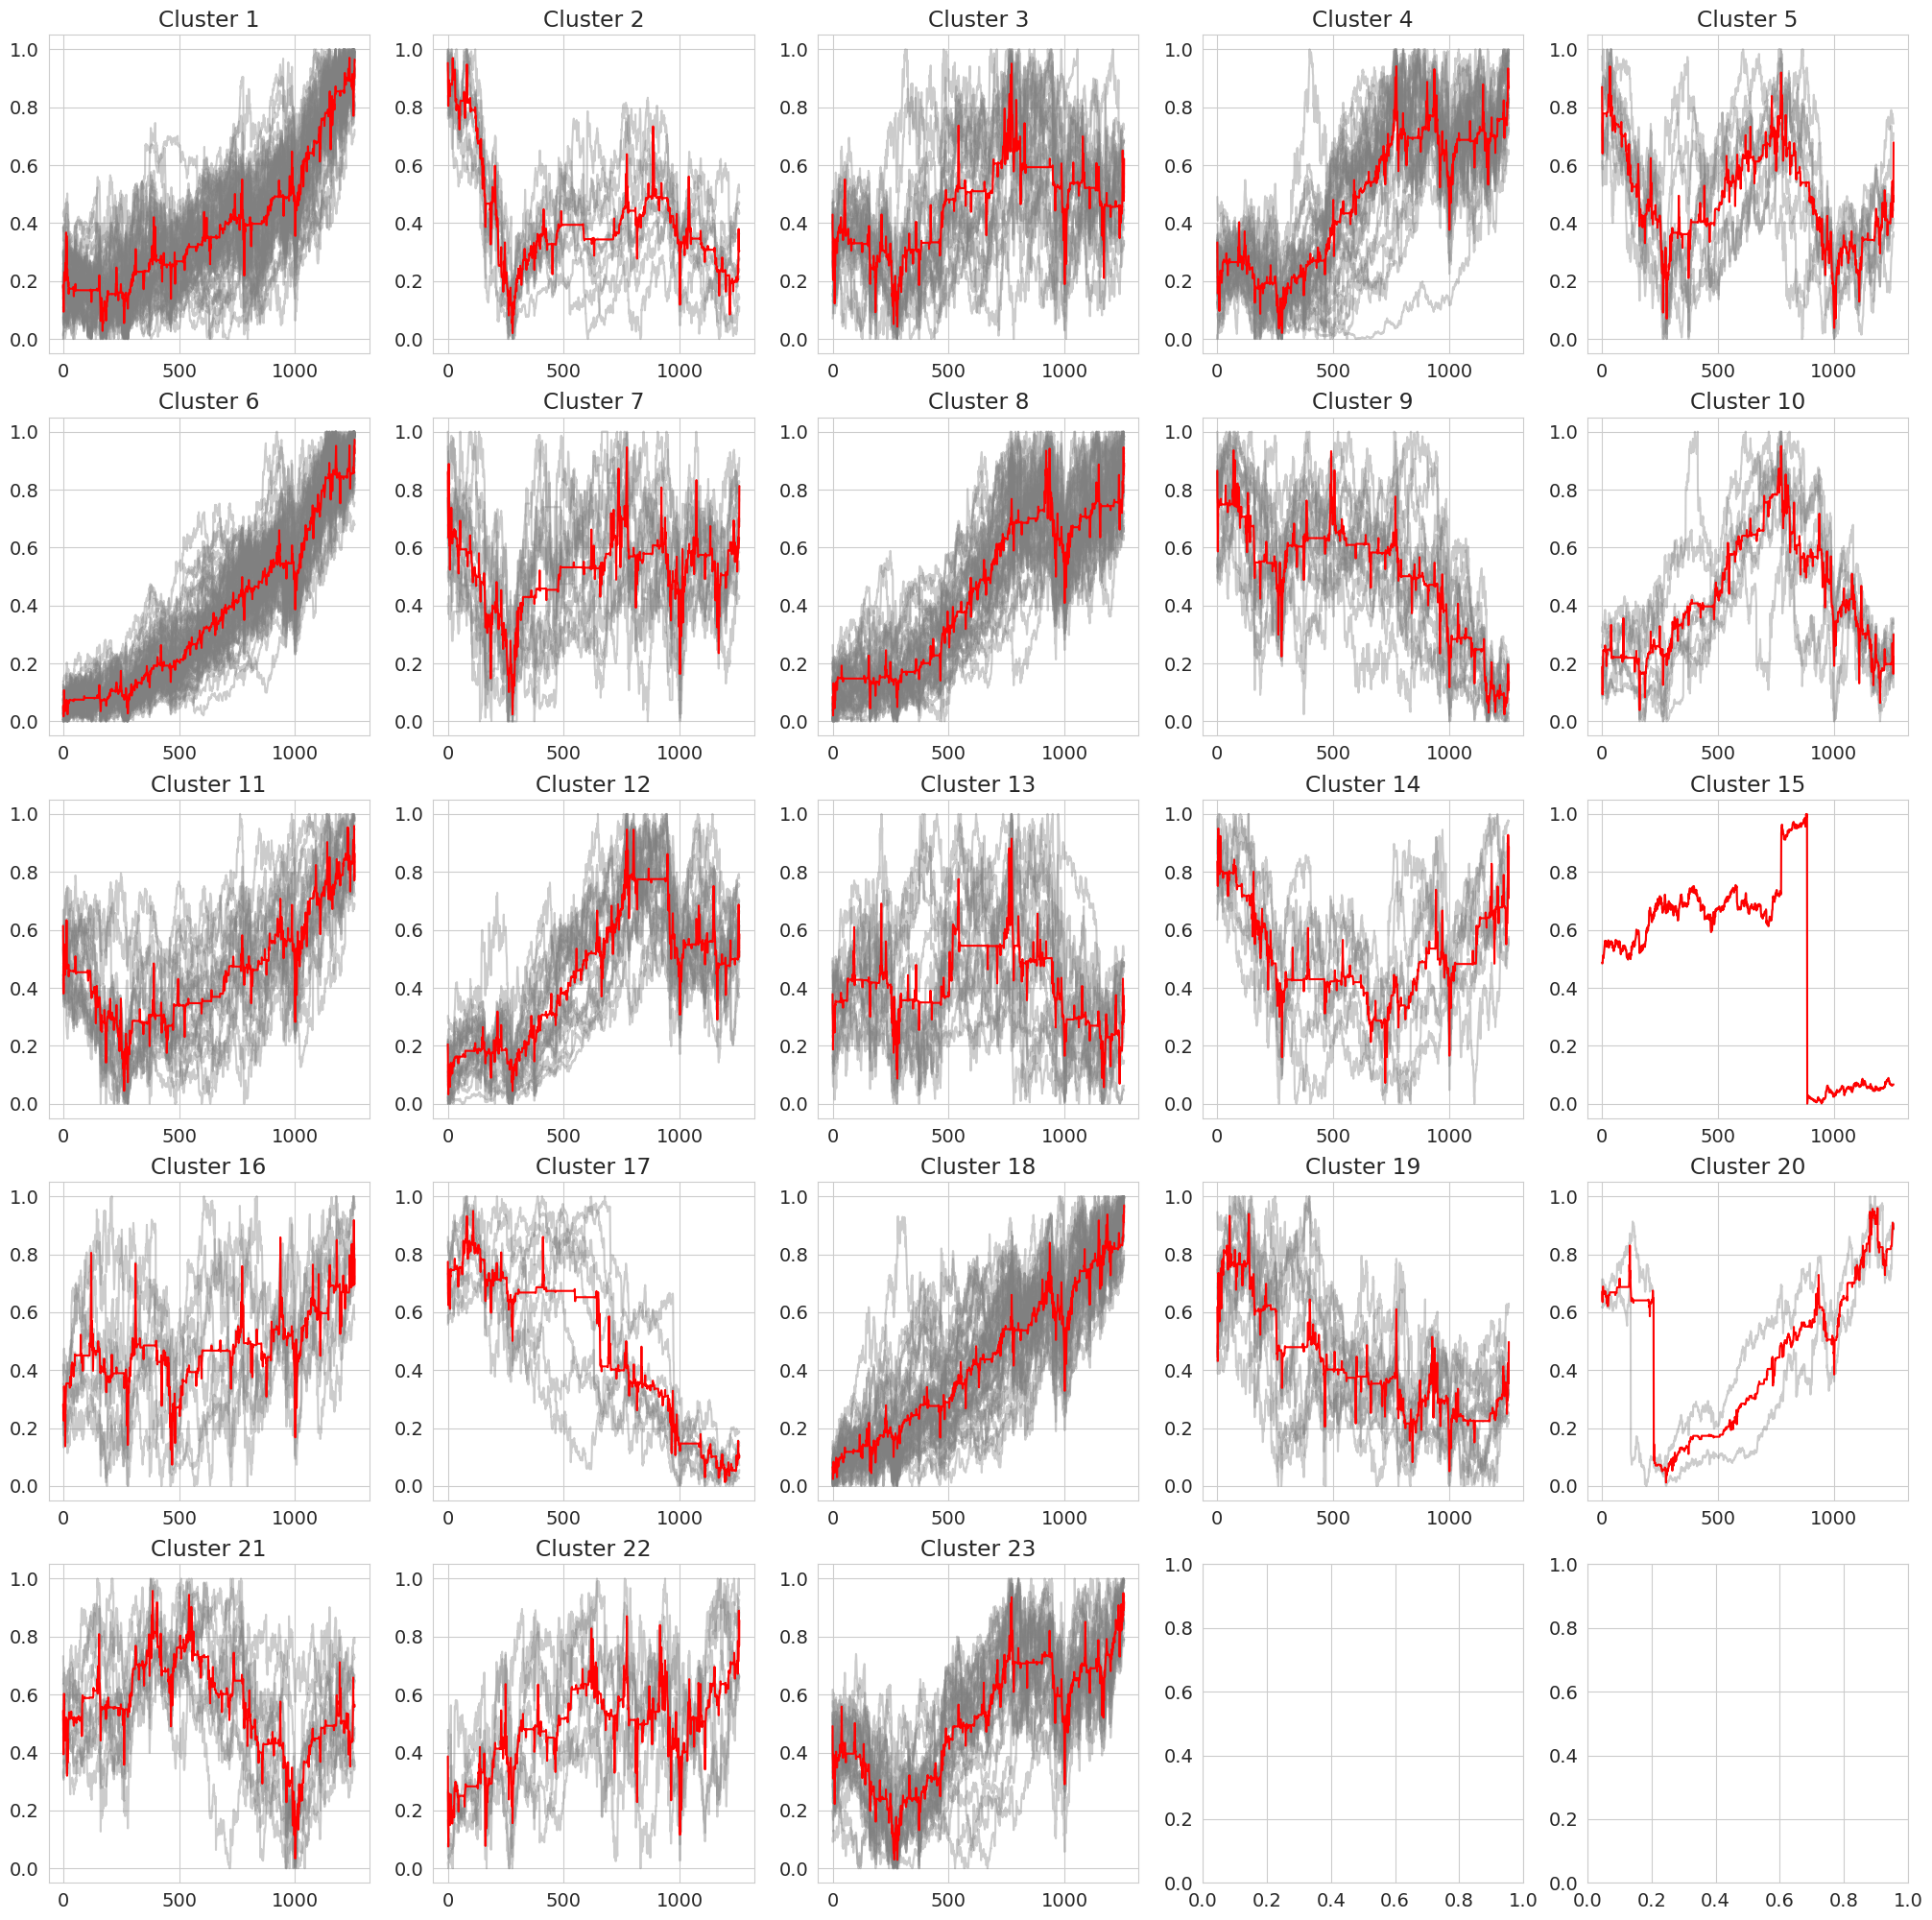
\includegraphics[width=12cm]{img/kmeands-ts-stocks-bary.png} 
\caption{K-Means DTW clusters with Barycenter intracluster line}
\label{fig:dtw_kmeans_bary}
\end{figure}

For visual evaluation, we have above the average centroid red line overlay in Fig. \ref{fig:dtw_kmeans_average} and the Barycenter overlay in  Fig. \ref{fig:dtw_kmeans_bary}. There are visually consistent patterns within each cluster's members (grey lines) when compared to the average (red line). This suggests that each cluster's average time-series correctly represents the general trend of its members.

Such is apparent in \textit{Cluster 3}: 

\begin{figure}[H]
\centering
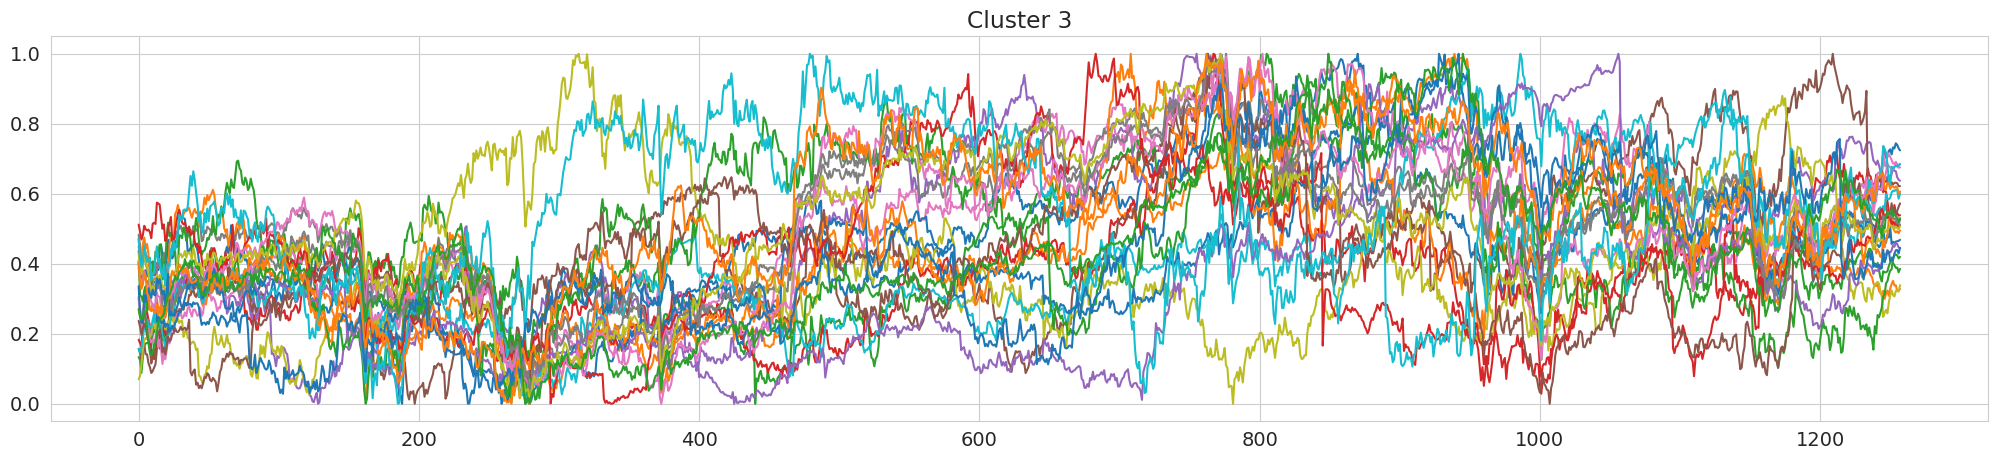
\includegraphics[width=12cm]{img/kmeans-dtw-cluster3.png} 
\caption{K-Means DTW Cluster 3}
\label{fig:kmeans_dtw_c3}
\end{figure}

There are also differences we can see between average lines and DBA lines, which emphasise how DBA is a better fit for DTW-generated clusters, as explained in the \textit{\hyperref[sec:compare]{Visual Inspection}} section. One such difference is observable in \textit{Cluster 22} in Fig. \ref{fig:dtw_kmeans_average} and Fig. \ref{fig:dtw_kmeans_bary}.


Interestingly, both K-Means DTW and the flat clusters approach have picked up on the same outlier (\textit{Cluster 20}), which MiniSom successfully managed to group with other stocks (Fig. \ref{fig:minisom_dba}).



K-Means DTW scored as follows in our tracked metrics:
\begin{itemize}
    \item \textit{Silhouette score:} 0.092
    \item \textit{Calinski-Harabasz index:} 8.359
    \item \textit{Davies-Bouldin index:} 1.813
\end{itemize}


A comparison of these scores for all algorithms can be found in the \textit{\hyperref[sec:compare]{Scoring and Comparison}} section.

The following bar chart illustrates the distribution of stocks across clusters:

\begin{figure}[H]
\centering
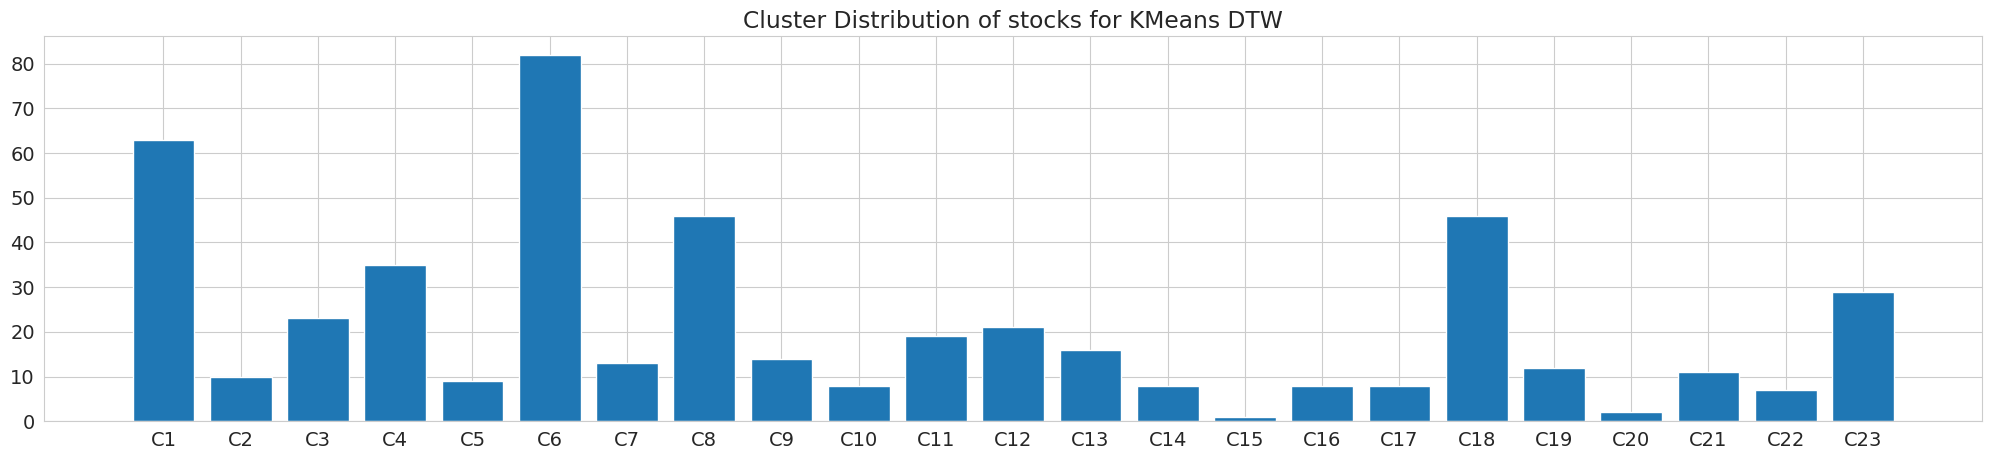
\includegraphics[width=12cm]{img/dtw-kmeans-distribution.png} 
\caption{Distribution of stocks within their K-Means DTW clusters}
\label{fig:dtw_kmeans_distribution}
\end{figure}


Most stocks were grouped under 5 notably dominant clusters (\textit{C1}, \textit{C6}, \textit{C8}, \textit{C18}, \textit{C23}), which suggests the algorithm could not find enough differentiating factors to generate a more uniform and valuable distribution. Two clusters contain only one or two individual stocks (\textit{C15} and \textit{C20}), due to their dissimilarity to all others due to the severe dip in price they have experienced in their history.

Without the stocks being split out by their patterns more evenly, it is unlikely for these groupings to be useful in a portfolio creation strategy, since marking 60 stocks as being similar does not give us enough confidence in a trend having been identified and the noisiness visualised showcases very unspecific trends. With only 5 majorly distinct behaviours identified in over 200 stocks, this algorithm may help capture the nuanced signals investors would be looking for.

\begin{figure}[H]
\centering
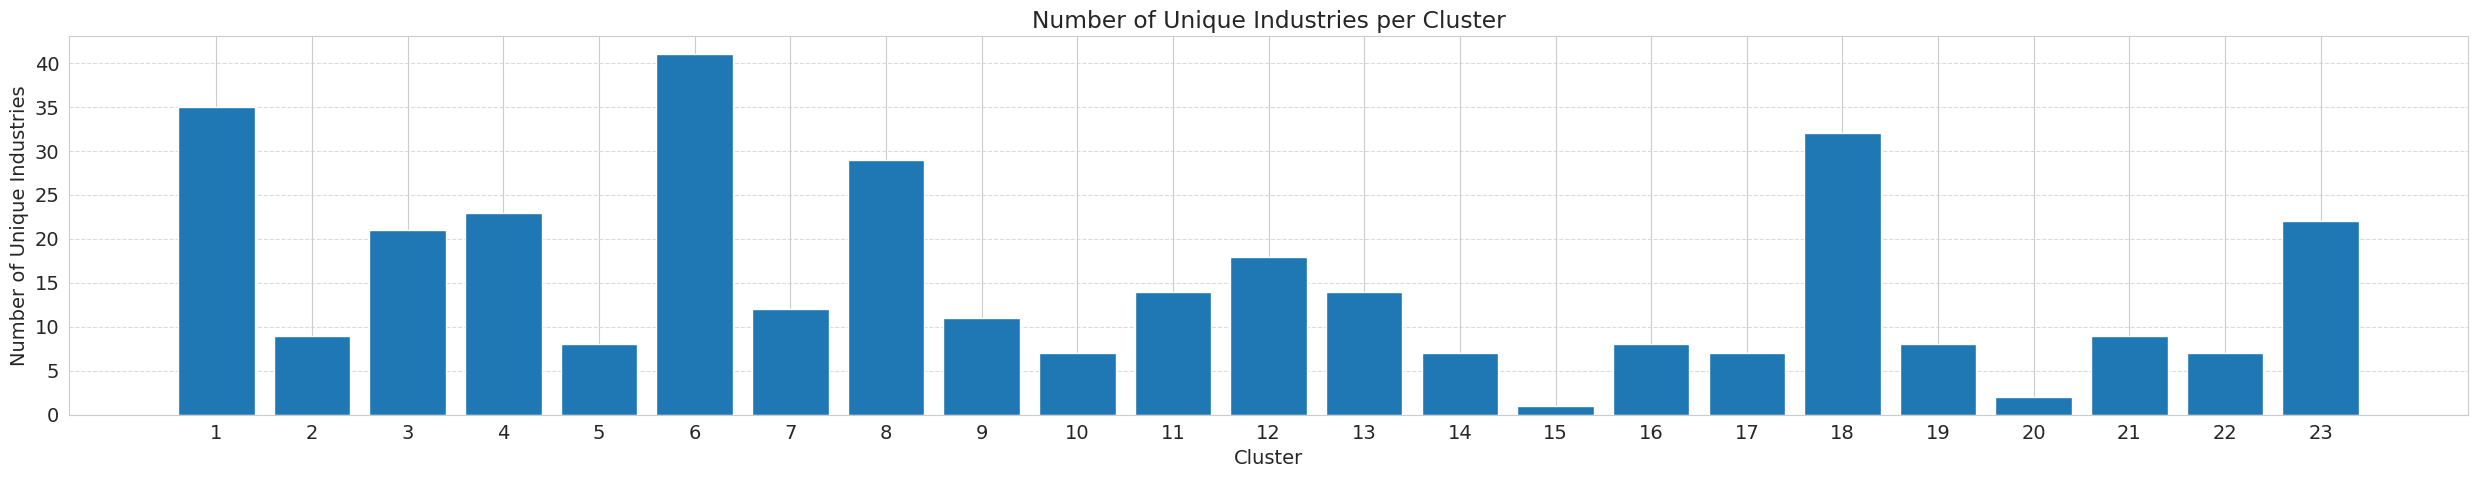
\includegraphics[width=12cm]{img/dtw-kmeans-industries.png} 
\caption{Distribution of industries within their K-Means DTW clusters}
\label{fig:dtw_kmeans_industries}
\end{figure}

Although the algorithm was not able to capture enough differentiating factors it was able to group stocks agnostic of their industry. As with the above algorithms, we see direct proportionality between the number of stocks and industries.

\subsubsection{Principal Component Analysis (PCA)}

In the models explored in previous sections, we consistently obtained outlying stocks that were not clustered with others. We decided to explore the use of Principal Component Analysis to reduce the complexity of our data and verify if leveraging the base K-Means algorithm would give us more effective and still-relevant clusters.

 High-dimensional data can be challenging for DTW since it computes pairwise distances between time-series. Reducing the dimensionality with PCA can make DTW computations more efficient without losing significant information.

 While PCA is a linear method and might not always capture complex non-linear relationships, in the context of normalised stock prices the main patterns (trends, volatility) can often be linear. This means PCA can help in retaining these patterns, making it easier for DTW to compute similarities.

\begin{figure}[H]
\centering
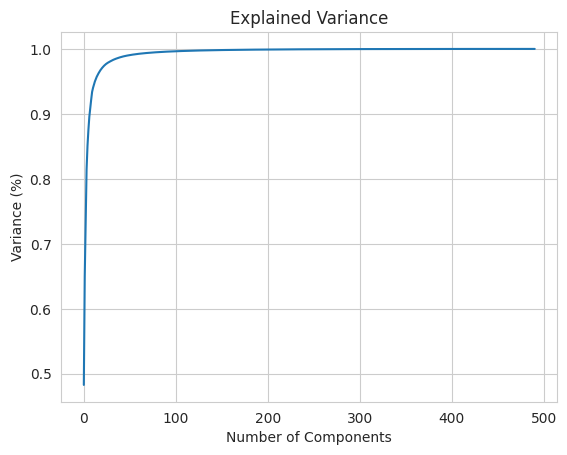
\includegraphics[width=7cm]{img/pca-variance.png} 
\caption{PCA variance analysis}

\end{figure}

 In the figure above, the x-axis represents the number of principal components, while the y-axis showcases the cumulative explained variance in percentage terms. 
 
 Near the  90-100 components mark, the rate variance growth starts to plateau. This elbow point suggests that adding more components would bring marginal returns as the graph almost saturates, indicating that further components add very little new information.



 After running the base K-Means algorithm on the data-set post-PCA, the resulting clusters were indeed slightly more uniform, with none of the clusters having one single stock:

\begin{figure}[H]
\centering
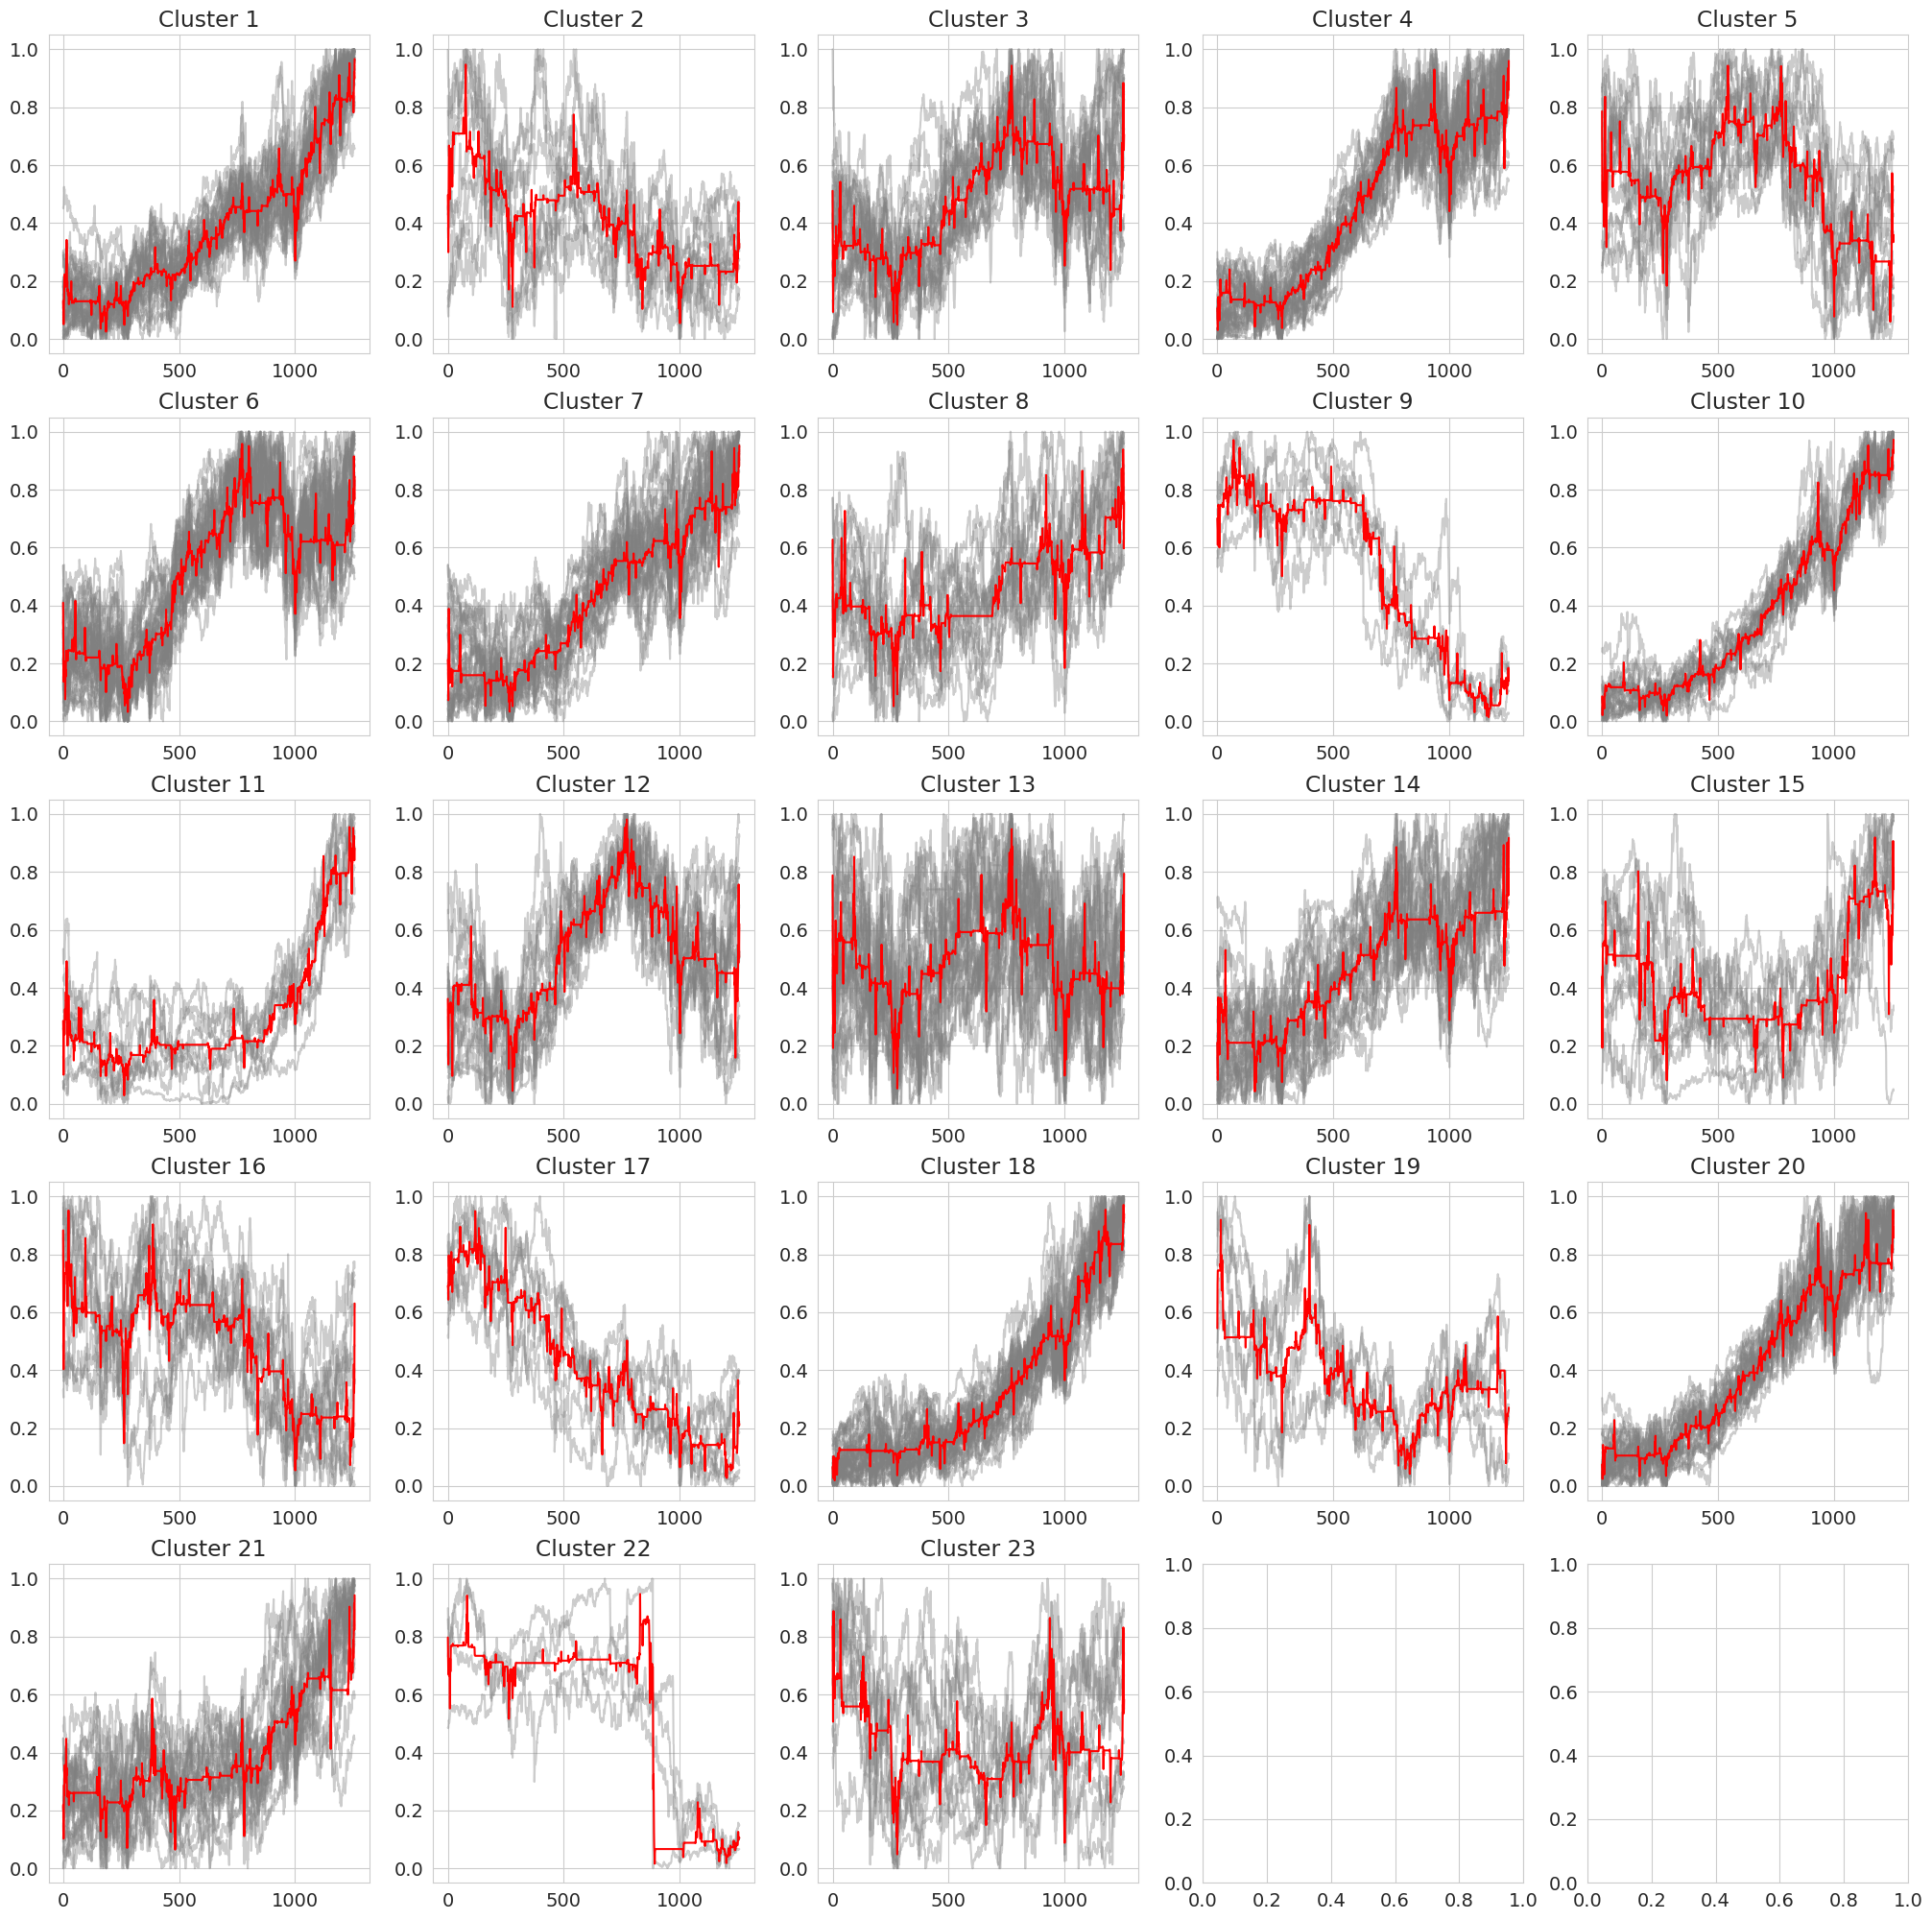
\includegraphics[width=12cm]{img/dbapca.png} 
\caption{Principal Component Analysis K-Means DTW clusters with DBA line}

\end{figure}


The outlier in \textit{Cluster 15} of Fig. \ref{fig:dtw_kmeans_bary} is now grouped with other stocks through PCA in \textit{Cluster 22}:

\begin{figure}[H]
\centering
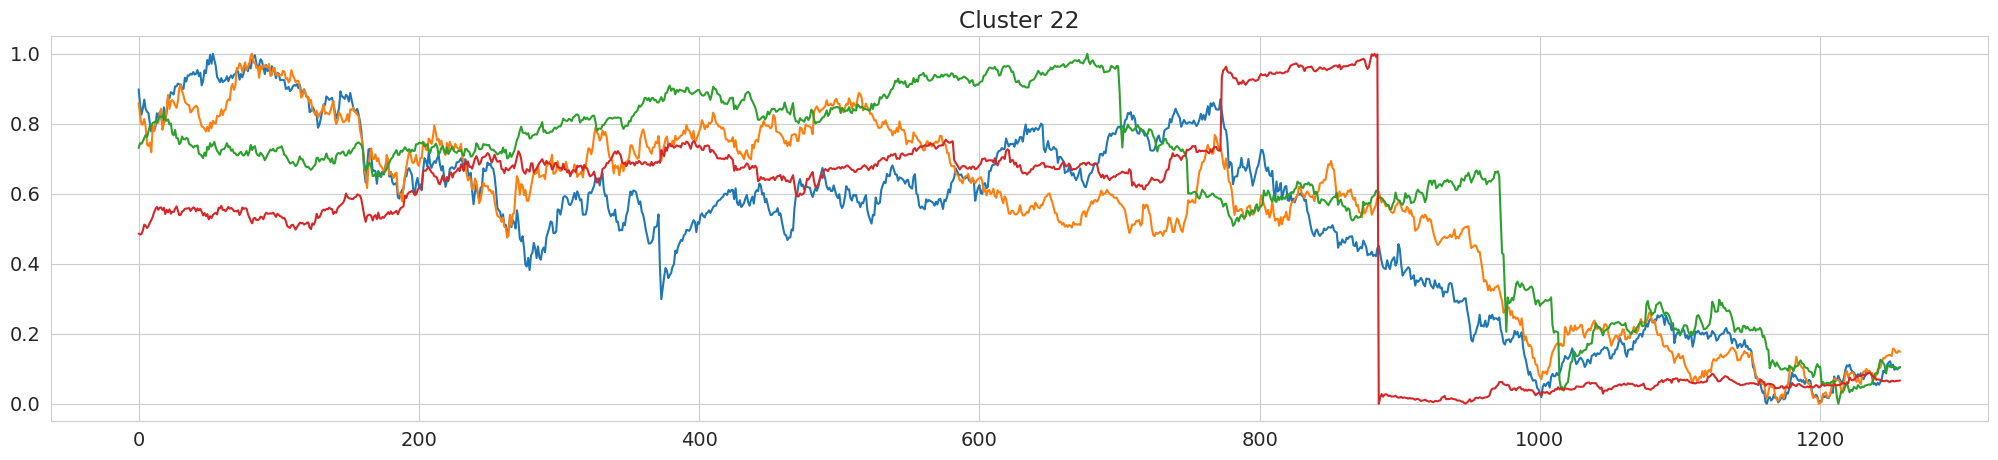
\includegraphics[width=12cm]{img/pca-cluster22.png} 
\caption{PCA - Cluster 22}
\end{figure}

Moreover, the distribution of stocks in clusters has improved as well:

\begin{figure}[H]
\centering
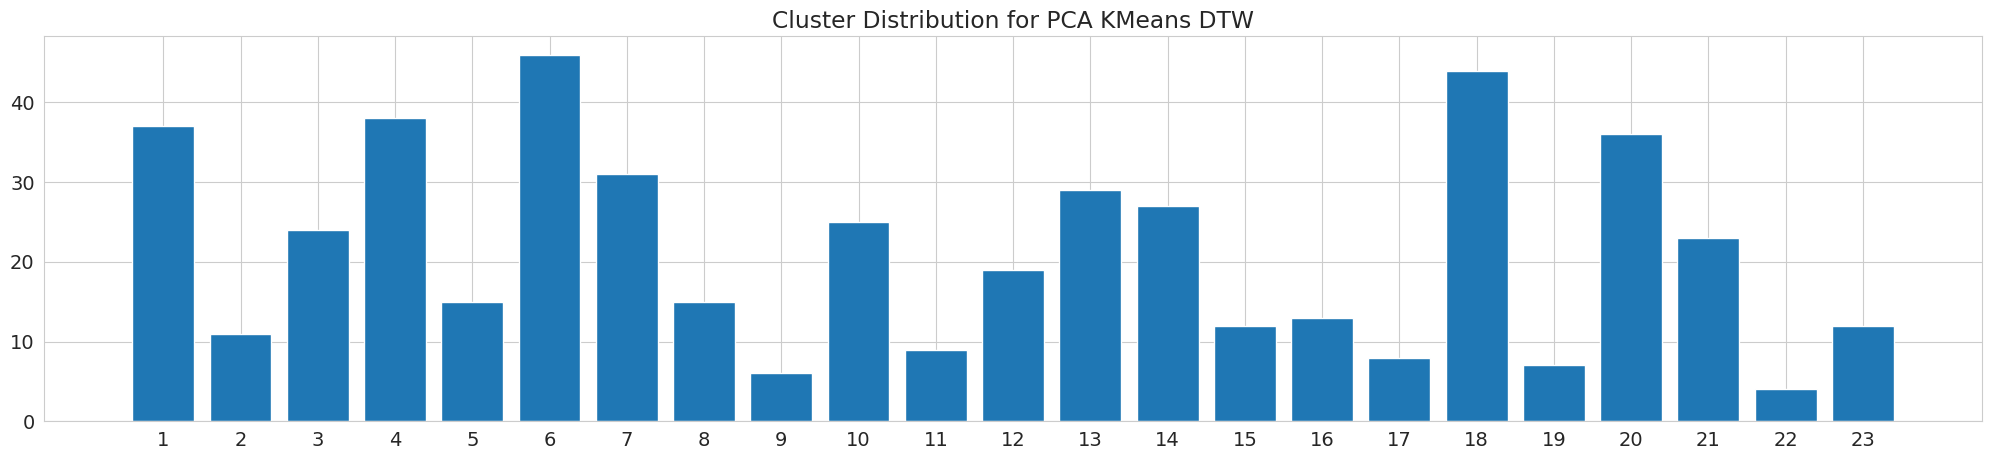
\includegraphics[width=12cm]{img/dtw-kmeans-pca-distribution.png} 
\caption{Distribution of stocks within their K-Means DTW PCA clusters}
\label{fig:dtw_kmeans_pca_distribution}
\end{figure}

The PCA approach on top of K-Means DTW helped improve how it identified differentiating factors. Instead of 5 dominating clusters (Fig. \ref{fig:dtw_kmeans_distribution}) we have generated a more uniform set of patterns that more closely resembles the MiniSom findings (Fig. \ref{fig:minisom_distribution}).

\begin{figure}[H]
\centering
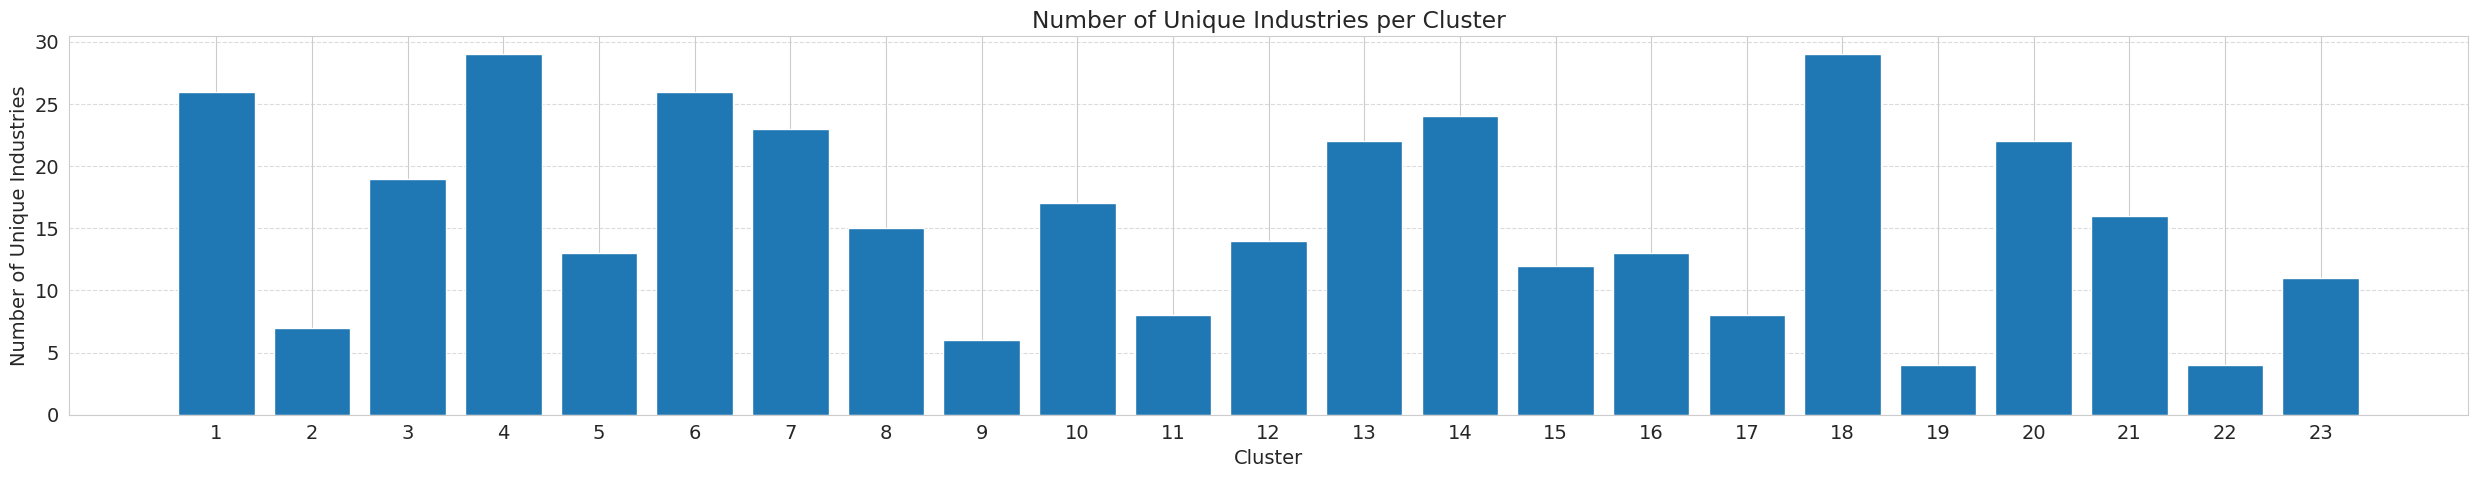
\includegraphics[width=12cm]{img/dtw-pca-industries.png} 
\caption{Distribution of industries in their K-Means DTW PCA clusters}
\label{fig:dtw_pca_industries}
\end{figure}

With direct relationships between the number of stocks and industries maintained, PCA improves upon K-Means DTW by more uniformly distributing stocks amongst clusters by finding more differentiating factors.


\subsection{Observations and Highlights}

An intriguing outcome of our exploration of the algorithms described above has been the generation of clusters that span over a couple of industries, showing that the behaviours of stocks can transcend the limitation of focusing on only one single category (ex. Fig. \ref{fig:minisom_industries}).

This indicates that rather than focusing on behaviours within a specific industry, it is worth tracking patterns across multiple industries and potentially formulating an investment strategy based on common industry patterns.  

\subsection{Scoring and Comparison}
\label{sec:compare}

\subsubsection{Silhouette score}

Cross-comparing the Silhouette scores of the methodologies we have explored and considering the highest numbers as a signal for the stock in each cluster being well matched to their cluster, we have reached the following ranking:


\begin{table}[H]
\centering
\begin{tabular}{|c|c|c|c|c|c|}
\hline
\textbf{Algorithm} & \textbf{Silhouette score} \\
\hline
DTW Flat Hierarchical & 0.116 \\
MiniSom & 0.11 \\
K-Means Euclidean & 0.109 \\
K-Means DTW & 0.092\\
\hline
\end{tabular}
\caption{Comparison of Algorithms via Silhouette score}
\label{tab:silhouette_Score}
\end{table}

The results for this particular metric classify MiniSom and DTW Flat clusters as the best. However, the differences between the scores are not heavily significant as the score ranges from -1 to 1 and our maximum difference between the top versus last ranking is 0.024.

We have heavily relied on visual observations to select the most appropriate clusters but found the Silhouette score valuable as an observation throughout the process to understand if we can impact it significantly and to understand potential correlations between the visuals we seek the the value of the score.

\subsubsection{Calinski-Harabasz Index}

By our secondary metric, the clustering methodologies ranked as follows:
\begin{table}[H]
\centering
\begin{tabular}{|c|c|c|c|c|c|}
\hline
\textbf{Algorithm} & \textbf{Calinski-Harabasz index} \\
\hline
MiniSom & 67.2 \\
K-Means Euclidean & 51.690 \\
K-Means DTW & 28.595\\
DTW Flat Hierarchical & 28.772 \\
\hline
\end{tabular}
\caption{Comparison of Algorithms via Calinski-Harabasz index}
\label{tab:calinski_score}
\end{table}

The Calinski-Harabasz index scoring most closely matched our visual observations, classifying the algorithms in the same order we have by analysing the clusters with their centroids in a graph.

    
\subsubsection{Davies-Bouldin Index}

The following table \ref{tab:davies_score} provides a comparative evaluation of various clustering algorithms based on the Davies-Bouldin index, a metric used to assess the quality of clustering. A lower Davies-Bouldin index suggests that the clusters are well-separated and thus, signifies a better clustering algorithm:

\begin{table}[H]
\centering
\begin{tabular}{|c|c|c|c|c|c|}
\hline
\textbf{Algorithm} & \textbf{Davies-Bouldin index} \\
\hline
K-Means Euclidean & 1.79 \\
MiniSom & 1.85 \\
K-Means DTW & 2.85\\
DTW Flat Hierarchical & 2.936 \\
\hline
\end{tabular}
\caption{Comparison of Algorithms via Davies-Bouldin index}
\label{tab:davies_score}
\end{table}

Alike to Calinski-Harabasz, the Davies-Bouldin index also fairly closely ranks the algorithms similarly to our visual conclusions.

\subsubsection{Visualisation}

Whilst we have selected mathematical metrics as empirical data for our assessment, we have also explored visualising the clusters within each section per algorithm. Due to the non-linear nature of the underlying stock data and the clusters we aim to form, it is non-trivial to establish a calculated metric that can be leveraged consistently throughout a diverse set of algorithms. Thus, we flag visualisations as the primary way to assess the outcomes generated in this work.

In Appendix \ref{allgraphs} we can see a comparison of all the generated clusters, with MiniSom having the most well-defined while still diverse and temporarily miss-aligned, as desired, outcome.

\section{Conclusions}
Investment strategy optimisation using stock clustering adapted for asynchronous patterns via Dynamic Time Warping algorithms and MiniSom is a powerful tool for investors looking to simplify the stock selection process and reduce risk. By clustering similar stocks together and analysing their historical performance, investors can identify investment opportunities and optimise their portfolio allocation. As we have seen through our visualisations of clusters above, using such algorithms allows investors to account for the time-dependent features of the stock prices and identify similar stocks that move together over time. While there are challenges associated with stock clustering and these approaches, such as the choice of clustering algorithm and distance metric, these challenges can be addressed using ensemble clustering techniques and careful analysis. With the right approach, investors can use stock clustering with DTW Flat Clusters from Hierarchical Clustering, K-Means DTW and MiniSom to make informed investment decisions and achieve their financial goals.


\subsection{Limitations}

One of the challenges of stock clustering is that it can be sensitive to the choice of clustering algorithm and distance metric. Different algorithms and metrics can produce different clusters, which can lead to different outliers and even varying investment opportunities. This challenge can be addressed using ensemble clustering techniques that combine multiple algorithms and metrics to produce more robust results.

Another challenge of stock clustering is that it is often performed on static data-sets, which does not account for changes in market conditions over time. This challenge can be addressed by using Dynamic Time Warping (DTW) and Self-Organising Maps (SOM) to measure the similarity between the historical performance of the stocks. These approaches take into account the time-dependent features of the stock prices, such as trends, cycles, and seasonality. This approach allows investors to identify similar stocks that move together over time, even if their prices fluctuate differently.

However, these algorithms can also be expensive. In our own use case, computational complexity meant we had to leverage parallel computing and often limit our ability to try too many variations of configurations due to the long-running time of algorithms.

\subsection{Overall Results}


\begin{table}[H]
\centering
\begin{tabular}{|c|c|c|c|c|c|}
\hline
\textbf{Algorithm} & \textbf{Silhouette} & \textbf{Calinski-Harabasz} & \textbf{Davies-Bouldin} \\
\hline
MiniSom & 0.11 & 67.2 & 1.85 \\
K-Means Euclidean & 0.109 & 51.69 & 1.789 \\
DTW Flat Hierarchical & 0.116  & 28.772 & 2.936 \\
K-Means DTW & 0.092 & 28.595 & 2.85\\
\hline
\end{tabular}
\caption{Comparison of mathematical scores across algorithms}
\label{tab:comparison_score}
\end{table}



\begin{itemize}
    \item \textbf{Flat Hierarchical} has moderate metrics across all categories, implying a balanced yet non-exceptional performance.
    \item \textbf{MiniSom} excels in the Calinski-Harabasz index and is most conclusive visually.
    \item \textbf{K-Means Euclidean} does not dominate on any metric or visually, used as our baseline.
    \item \textbf{K-Means DTW} performs poorly across all metrics, indicating that this algorithm is less effective in forming well-defined and distinct clusters.
\end{itemize}


Based on the data in Table \ref{tab:comparison_score} and the scoring metrics we have chosen, K-Means Euclidean emerges as the best-performing algorithm, albeit not very dominant, for stock clustering. This is primarily due to the metrics themselves being much better suited to detect when Euclidean matching has been done effectively.

However, if we consider visual comparison as the main factor to measure the success of the clustering algorithms, MiniSom most successfully matches clusters together with clear smooth trends visible, making it a great algorithm for practical applications (Appendix \ref{allgraphs}). 

\subsection{Room for Improvement}

There are opportunities to study the clusters quarter by quarter to check cluster consistency. As most companies divide their fiscal year into quarters and measure their performance on the same, we might find that they behave similarly in one financial quarter but not in all. 

The preceding sections have elaborated on the efficiency and reliability of various clustering algorithms, such as DTW Flat Clusters From Hierarchical Clustering, MiniSom, K-Means, and K-Means DTW, in the realm of stock analysis. While these algorithms offer promising results, as indicated by metrics like the Silhouette score, Davies-Bouldin index, and Calinski-Harabasz index, there exists ample scope for improvement. This chapter seeks to explore these areas of potential enhancement.

\subsubsection{Inclusion of Additional Features}

Current methodologies primarily focus on historical stock prices and their time-dependent features. The inclusion of more comprehensive features such as trading volumes, dividend yields, and external economic indicators could offer a more holistic view of stock behaviour. Subsequently, PCA optimisations to reduce dimensionality will add even more value for K-Means and MiniSom which are already designed to work with multiple dimensions.

\subsubsection{Robustness to Market Volatility}

Stock markets are subject to a multitude of factors that contribute to their volatility. The adaptability of the clustering algorithms to rapidly changing market conditions needs to be enhanced. Employing more dynamic models that can update the clusters in real time might be an avenue worth exploring.

\subsubsection{Interpretability and Usability}

While high scores on performance metrics indicate good clustering, the true test of a model's utility is its ease of interpretation and implementation by stakeholders. A focus on creating more transparent and easy-to-use models can bridge the gap between mathematical robustness and practical applicability.

We would like to identify an algorithm for backtesting by simulating trades over a certain period and informing the decision-making process by using the generated clusters from the different methodologies as similarly done by Sáenz, Quiroga, and Barivier in \textit{Data vs. information: Using clustering techniques to enhance stock returns forecasting} \cite{dataVsInformation}. 

Investors can use various techniques to further analyse the clusters and backtest, such as mean-variance optimisation, factor analysis, or Monte Carlo simulation. Mean-variance optimisation aims to find the optimal portfolio allocation that maximises expected returns while minimising risk. Factor analysis identifies the underlying factors that drive the clusters' performance, such as industry trends or macroeconomic indicators. Monte Carlo simulation simulates various market scenarios to estimate the potential returns and risks of the different investment strategies.



\subsection{Concluding Remarks}

The techniques presented in this paper are informative to an investment or trading strategy, but not recommended as stand-alone signals. Instead, they should be used as a weighted indicator, contributing to a more holistic analysis that takes into account other signals and leverages clusters to understand the likelihood of cross-industry stocks behaving asynchronously similarly.

This study has demonstrated the efficacy of Mini Self-Organising Map (Minisom) as a method for clustering stocks. Unlike traditional distance metrics, SOM captured intricate time-dependent patterns and phase shifts that are inherent in financial time-series data. The findings have significance for portfolio management, risk assessment, and algorithmic trading, offering a more nuanced understanding of stock asynchronous behaviour patterns.

Whilst the SOM method created the smoothest clusters and had a good distribution of stocks in the clusters without outliers, K-Means DTW did successfully identify common trends across stocks at asynchronous points in time, albeit with more noise than SOM. Despite this, its ability to successfully group stocks non-linearly makes it another method that could prove useful for financial analysts. 

However, it is worth noting that DTW-based clustering comes with computational constraints, which is a limiting factor for real-time analysis involving large data-sets. Future research may focus on testing approximations and lighter versions of DTW algorithms. 

Finally, our use-case only uses one dimension: closing price. Integrating other variables as simple as trade volume and as complex as market sentiment or macroeconomic indicators could provide a more holistic approach to stock clustering, especially with the ever-increasing complexity and volatility of financial markets. In that regard, DTW and SOM-based clustering represents a promising frontier for both academic inquiry and practical applications in finance, compatible with low and high data dimensionality.


\newpage

\section{References}

\printbibliography[title={~}]



% Activate the appendix in the doc
% from here on sections are numerated with capital letters 
\begin{appendices}

\section{GitHub Project} \label{github}

The GitHub project has the Jupyter Notebook, data and tools used to generate the results and visualisations in this paper.

\url{https://github.com/nenuadrian/msc-business-analytics-dissertation}


\section{Results from all clusters} \label{allgraphs}

\begin{figure}[H]
\centering
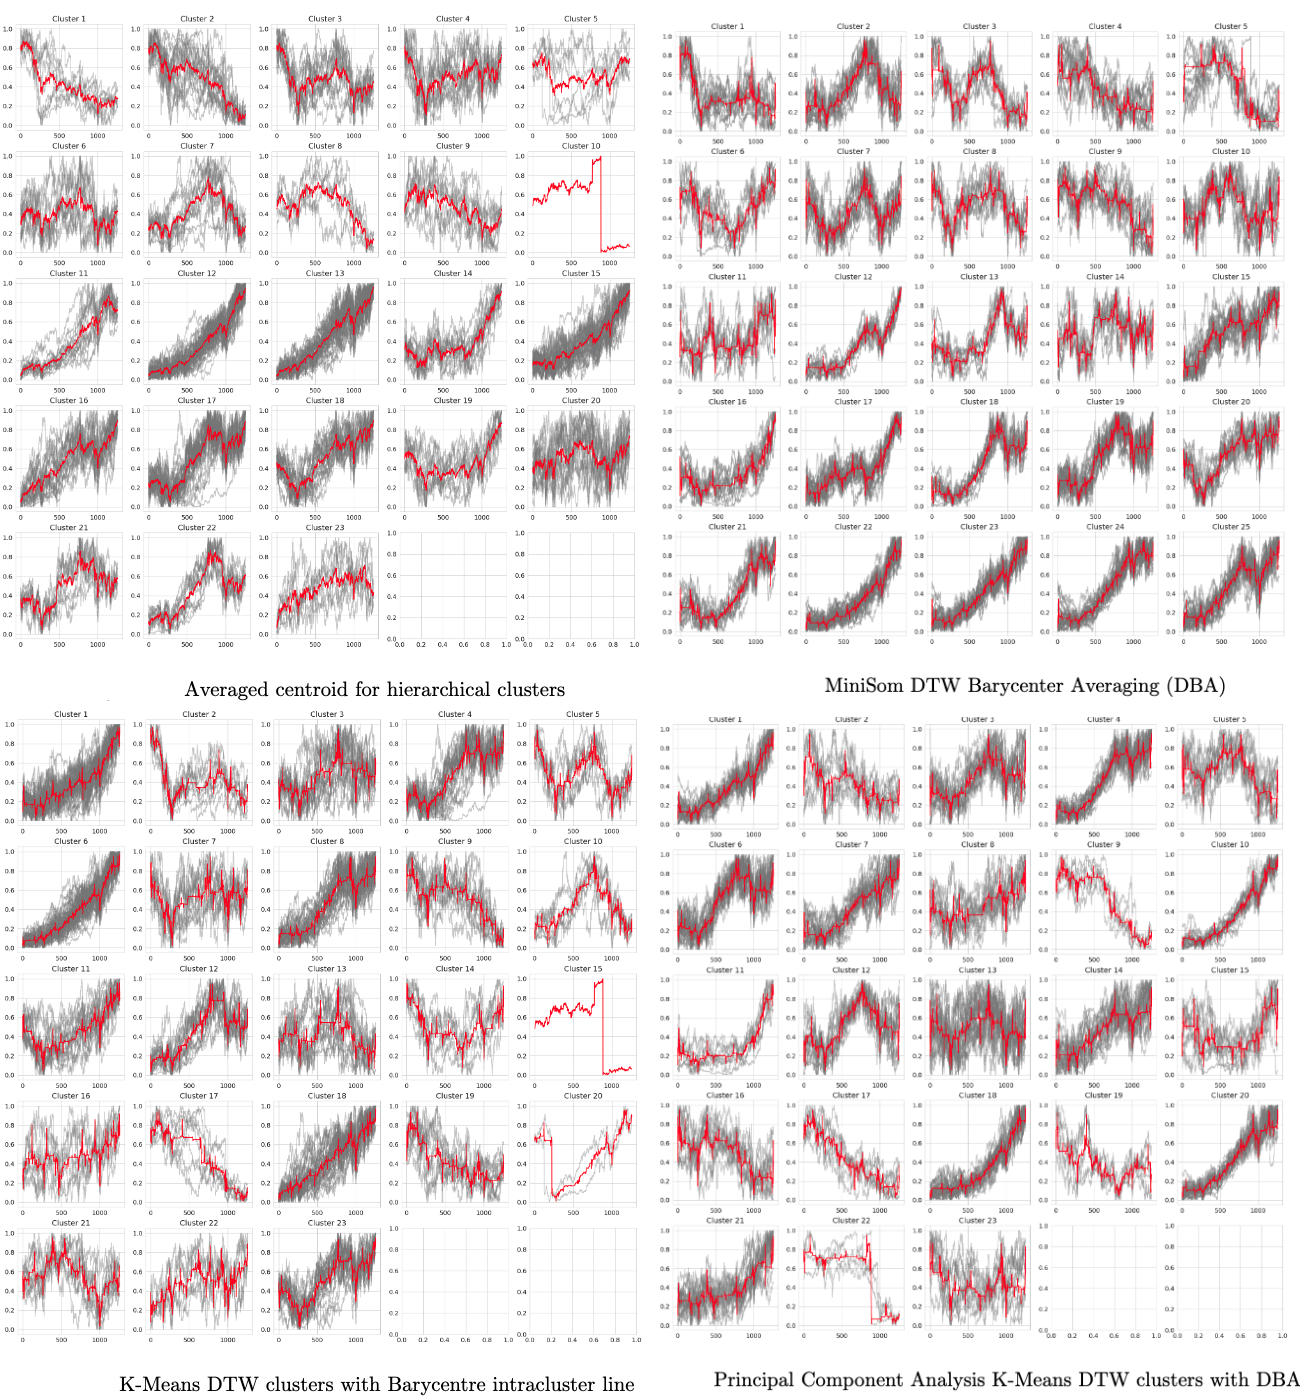
\includegraphics[width=15cm]{img/allgraphs.jpeg} 
\caption{Results from all clusters for visual comparison}
\label{fig:all_graphs}
\end{figure}





\end{appendices}

\end{document}
